% THIS IS AN EXAMPLE DOCUMENT FOR VLDB 2012
% based on ACM SIGPROC-SP.TEX VERSION 2.7
% Modified by  Gerald Weber <gerald@cs.auckland.ac.nz>
% Removed the requirement to include *bbl file in here. (AhmetSacan, Sep2012)
% Fixed the equation on page 3 to prevent line overflow. (AhmetSacan, Sep2012)

\documentclass{vldb}
\usepackage{graphicx}
\graphicspath{ {images/} }
\usepackage{balance}  % for  \balance command ON LAST PAGE  (only there!)
\usepackage{amsmath}
\usepackage{url}
\usepackage{subcaption}
\usepackage{amsmath}
\usepackage[utf8]{inputenc}
\usepackage{booktabs,floatrow}

\usepackage[linesnumbered,ruled]{algorithm2e}
\SetKwRepeat{Do}{do}{while}%


\begin{document}
\newcommand{\argmin}{\operatornamewithlimits{argmin}}
\newcommand{\argmax}{\operatornamewithlimits{argmax}}

% ****************** TITLE ****************************************

\title{ Performance Evaluation of Stream Data Processing Systems}

% possible, but not really needed or used for PVLDB:
%\subtitle{[Extended Abstract]
%\titlenote{A full version of this paper is available as\textit{Author's Guide to Preparing ACM SIG Proceedings Using \LaTeX$2_\epsilon$\ and BibTeX} at \texttt{www.acm.org/eaddress.htm}}}

% ****************** AUTHORS **************************************

% You need the command \numberofauthors to handle the 'placement
% and alignment' of the authors beneath the title.
%
% For aesthetic reasons, we recommend 'three authors at a time'
% i.e. three 'name/affiliation blocks' be placed beneath the title.
%
% NOTE: You are NOT restricted in how many 'rows' of
% "name/affiliations" may appear. We just ask that you restrict
% the number of 'columns' to three.
%
% Because of the available 'opening page real-estate'
% we ask you to refrain from putting more than six authors
% (two rows with three columns) beneath the article title.
% More than six makes the first-page appear very cluttered indeed.
%
% Use the \alignauthor commands to handle the names
% and affiliations for an 'aesthetic maximum' of six authors.
% Add names, affiliations, addresses for
% the seventh etc. author(s) as the argument for the
% \additionalauthors command.
% These 'additional authors' will be output/set for you
% without further effort on your part as the last section in
% the body of your article BEFORE References or any Appendices.

%\numberofauthors{8} %  in this sample file, there are a *total*
% of EIGHT authors. SIX appear on the 'first-page' (for formatting
% reasons) and the remaining two appear in the \additionalauthors section.

%\author{
% You can go ahead and credit any number of authors here,
% e.g. one 'row of three' or two rows (consisting of one row of three
% and a second row of one, two or three).
%
% The command \alignauthor (no curly braces needed) should
% precede each author name, affiliation/snail-mail address and
% e-mail address. Additionally, tag each line of
% affiliation/address with \affaddr, and tag the
% e-mail address with \email.
%
% 1st. author
%\alignauthor
%Ben Trovato\titlenote{Dr.~Trovato insisted his name be first.}\\
%   \affaddr{Institute for Clarity in Documentation}\\
%   \affaddr{1932 Wallamaloo Lane}\\
%   \affaddr{Wallamaloo, New Zealand}\\
%   \email{trovato@corporation.com}
%% 2nd. author
%\alignauthor
%G.K.M. Tobin\titlenote{The secretary disavows
%any knowledge of this author's actions.}\\
%   \affaddr{Institute for Clarity in Documentation}\\
%   \affaddr{P.O. Box 1212}\\
%   \affaddr{Dublin, Ohio 43017-6221}\\
%   \email{webmaster@marysville-ohio.com}
%% 3rd. author
%\alignauthor Lars Th{\Large{\sf{\o}}}rv{$\ddot{\mbox{a}}$}ld\titlenote{This author is the
%one who did all the really hard work.}\\
%   \affaddr{The Th{\large{\sf{\o}}}rv{$\ddot{\mbox{a}}$}ld Group}\\
%   \affaddr{1 Th{\large{\sf{\o}}}rv{$\ddot{\mbox{a}}$}ld Circle}\\
%   \affaddr{Hekla, Iceland}\\
%   \email{larst@affiliation.org}
%\and  % use '\and' if you need 'another row' of author names
%% 4th. author
%\alignauthor Lawrence P. Leipuner\\
%   \affaddr{Brookhaven Laboratories}\\
%   \affaddr{Brookhaven National Lab}\\
%   \affaddr{P.O. Box 5000}\\
%   \email{lleipuner@researchlabs.org}
%% 5th. author
%\alignauthor Sean Fogarty\\
%   \affaddr{NASA Ames Research Center}\\
%   \affaddr{Moffett Field}\\
%   \affaddr{California 94035}\\
%   \email{fogartys@amesres.org}
%% 6th. author
%\alignauthor Charles Palmer\\
%   \affaddr{Palmer Research Laboratories}\\
%   \affaddr{8600 Datapoint Drive}\\
%   \affaddr{San Antonio, Texas 78229}\\
%   \email{cpalmer@prl.com}
%}
% There's nothing stopping you putting the seventh, eighth, etc.
% author on the opening page (as the 'third row') but we ask,
% for aesthetic reasons that you place these 'additional authors'
% in the \additional authors block, viz.

\date{30 July 1999}
% Just remember to make sure that the TOTAL number of authors
% is the number that will appear on the first page PLUS the
% number that will appear in the \additionalauthors section.


\maketitle
\begin{abstract}
Over the past years, Stream Data Processing is gaining compelling attention both in industry and in academia due to its wide range of applications in various use-cases. To fulfil the need for efficient and high performing  Big Data analytics, numerous open source Stream Data Processing Systems (SDPS) were developed. Processing data with high throughput while retaining low latency is key performance indicator for such systems. In this paper, we propose a benchmarking system to evaluate the performance of SDPSs, Storm, Spark and Flink  in terms of latency and throughput. More specifically, the latency of windowed aggregation and windowed join operators is evaluated jointly  with the throughput of a system. The main goal of this work is to build a benchmarking system for SDPS which is simple because simple is beautiful.  The main contribution of this work is threefold. Firstly, we first define a definition of latency and throughput for stateful operators, based on the industry use-case. Secondly, we completely separate the unit under test and driver. This enables us not only building a simple and transparent system but also empowers the system to be flexible. Finally, we first build a driver to test the sustainability of a unit under test which supports various user defined policies. 

\end{abstract}

\section{Introduction}
Processing large volumes of data in batch is often not sufficient in cases where new data has to be processed fast to quickly adapt and react to changes. For that reason, stream data processing (SDP) has gained significant attention. The most popular engines used for SDP, with large-scale adoption by industry and the research community, are Apache Storm \cite{toshniwal2014storm}, Apache Spark  \cite{zaharia2012discretized}, and Apache Flink \cite{carbone2015apache}. 

\begin{figure*}
    \centering
    \begin{subfigure}[b]{0.3\textwidth}
        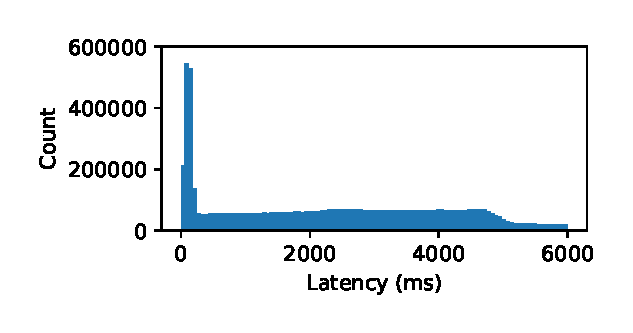
\includegraphics[width=\textwidth]{2nodesize2_hist}

        \caption{Storm, 2-node, max  throughput }
    \end{subfigure}
    ~ 
    \begin{subfigure}[b]{0.3\textwidth}
        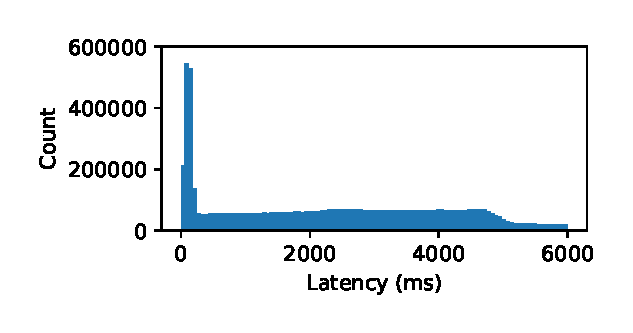
\includegraphics[width=\textwidth]{2nodesize2_hist}

        \caption{Storm, 4-node, max   throughput }
    \end{subfigure}
    ~ 
    \begin{subfigure}[b]{0.3\textwidth}
        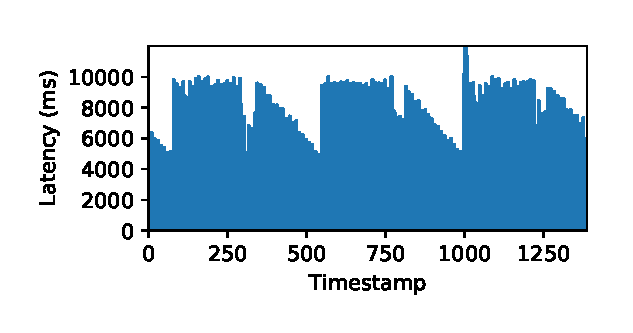
\includegraphics[width=\textwidth]{2nodesize2_ts}

        \caption{Storm, 8-node, max  throughput }
        
    \end{subfigure}
\end{figure*}

One  important application area of SDP is  online video games. These require the fast processing  of large scale online data feeds  from different sources. Windowed aggregations and windowed joins are two main operations that are used to monitor user feeds. One typical use-case is tracking the in-application-purchases (IAPs) per application, per distribution channel, or per product item (in-app products). Another typical use-case is the monitoring of advertising:  making sure that all campaigns and advertisement networks work flawlessly. Yet another use-case is comparing different user feeds by  joining them. For example, monitoring the IAPs of the same game downloaded from different distribution channels and comparing users'  actions  are essential in  online video game monitoring.


% \todo[inline]{Try to reflect Henri's comments: I suggest to first describe the jobs generically, i.e., aggregations and joins, and then relate them to the online game use cases of Rovio that Henri described (both what they do and what they plan to do).=>fixed}

In this work, we propose a benchmarking framework to accurately measure the performance of stream data processing engines. For our experimental evaluation, we test three publicly available open source and community driven engines, namely Apache Storm, Apache Spark, and Apache Flink.  
We measure the latency and throughput as the major performance indicators. Latency, in SDP, is the time difference between data production at the source (e.g., the mobile device) to result output at the sink of the data flow graph describing the stream processing operations (e.g., the monitoring solution on the game server). Throughput, in this scenario, determines the number of ingested and successfully processed records or events per time unit.

%In this paper we inspired from the quote of Napoleon Bonaparte being "Ability is nothing without opportunity". 
%Giving opportunity to all systems to express their ability is the key in benchmarking. 
Even though there have been several comparisons of the performance of SDPS recently, these do not measure the latencies and throughput that can be achieved in a production setting. One of the repeating problems in the previous evaluations is a missing definition and inaccurate measurement procedure for latency of stateful operators in SDPS. Another challenge is a missing separation between the system under test (SUT) and the benchmark driver. Frequently, the performance metrics are measured and calculated within SUT; this means that the results will be influenced through the measurements and, thus, can be biased. %Another challenge is, enabling the driver to be flexible enough to support different policies to handle system specific features. For example, back-pressure is characteristic feature of SDPSs and while calculating a system's sustainability with a given workload, it must be taken into consideration. Most importantly, it is essential to  keep the benchmarking system simple while solving the challenges listed above
We discuss in detail these challenges as well as our solutions in Section \ref{chal}.


% For example, there are numerous open challenges related with measuring main Key Performance Indicators (KPIs) in stream data processing engines. One of them is lacking the clear definition for the latency of stateful operator in SDPS.   The stream and its output are theoretically infinite and, therefore, the methods to measure its latency  have to be different from the batch processing systems. While the some works \cite{chintapalli2016benchmarking}, checkpoint events' timestamps in another system, this can  escalate the driver's complexity and create \textit{artificial latency}. Although the authors define latency as an average time span from the arrival of record till the end of its processing \cite{lu2014stream}, this definition is optimistic. In real life scenarios, the actual latency is calculated from the event's generation time. Moreover, when benchmarking SDPSs, it is crucial to separate the driver and system under test completely as otherwise, the results can be biased \todo[inline]{why?}. Furthermore, the driver should be flexible enough to support different policies to handle system specific features. For example, back-pressure is characteristic feature of SDPSs and while calculating a system's sustainability with a given workload, it must be taken into consideration.
%Most importantly, it is essential to  keep the benchmarking system simple while solving the challenges listed above. 

In this paper, we address the above mentioned challenges. The proposed solution is generic, has a clean design with clear semantics, and can be applied to any SDPS. The main goal is to stimulate an environment in which we can measure the metrics more precisely and with minimum influence of side factors.

The main contributions of this paper go as follows:
\begin{itemize}  
\item We    introduce a mechanism to accurately measure the latency of stateful operators in SDPSs. We apply the proposed method to use-cases featuring windowed aggregations and windowed joins. 
\item We accomplish the complete separation of the test driver from the system under test (SUT). 
 %\todo[inline]{the second sentence is unclear=>deleted}
\item We measure the maximum sustainable throughputs of the SDPSs. Our benchmarking framework handles system specific features like backpressure to measure the maximum sustainable throughput of a system. 
%\item We accomplish the above contributions with a simple system design with minimum components being System Under Test (SUT) and Data Engine. 
\item We use the proposed benchmarking system for an extensive evaluation of Storm, Spark, and Flink with practical use-cases.
\end{itemize}

The remainder of this paper is organized as follows. In Section \ref{rel}, we survey the related work. We give an overview of the stream data processing engines benchmarked in this paper in Section \ref{pre}. In Section \ref{chal}, we discuss the detailed interpretation of stream benchmarking challenges and their importance. We provide the design of our benchmarking system, the use-cases, and the metrics in Section \ref{des}. After a detailed evaluation in Section \ref{eval}, we conclude in Section \ref{conc}.

\section{Related work}
The main concepts and methodologies used in benchmarking SDPS were inherited from big data benchmarks.
Now with emerging next generation stream data processing engines, batch processing is seen as a special case of stream processing where the data size is bounded. Huang et.al. propose HiBench, the first benchmark suite for evaluation and characterisation of Hadoop \cite{white2012hadoop}. Authors conduct wide range of experiments from micro-benchmarks to machine learning algorithms \cite{huang2011hibench}. Covering end-to-end big data benchmark with all major characteristics such as three Vs in the lifecycle of big data systems is the main intuition behind BigBench \cite{ghazal2013bigbench}. Wang et.al. introduce BigDataBench, a big data benchmark suite for Internet Services, characterising the 19 big data benchmarks covering broad application scenarios and diverse and representative data sets \cite{wang2014bigdatabench}.

 Benchmarks on SDPS are  Researchers from Yahoo Inc. have done benchmarks on streaming systems to measure latency and throughput \cite{chintapalli2016benchmarking}. They used Apache Kafka \cite{kafka2014high} and Redis \cite{carlson2013redis} for data fetching and storage. Later on, on the other hand, Data Artisans, showed those systems actually being a bottleneck for SUT's performance \cite{dataartisans}.  The extensive analysis of the differences between Apache Spark and Apache Flink in terms of batch processing is done by correlating the operators execution plan with the resource utilization and the parameter configuration \cite{marcu2016spark}. In another benchmark, authors compare the performances of Apache Spark and Apache Flink to  provide clear, easy and reproducible configurations that can be validated by community in clouds \cite{perera2016reproducible}. Authors conducted  benchmarks to assess the fault tolerance and throughput efficiency for open source stream data processing engines \cite{lopez2016performance}. In another benchmark, authors motivate IoT as being main application area for SDPS and perform common tasks in particular are with different stream data processing engines and evaluate performance \cite{shukla2016benchmarking}. One of the pioneers in SDPS benchmarks, developed framework StreamBench analysing the current standards in streaming benchmarks and proposing a solution to measure throughput, latency considering the fault tolerance of SUT \cite{lu2014stream}. Authors put a mediator system between data generator module and SUT and define the latency as the average time span from the arrival of a record till the end of processing of the record. LinearRoad benchmarking framework was presented by Arasu et al. to measure performance of standalone stream data management systems such as Aurora \cite{abadi2003aurora} by simulating a scenario of toll system for motor vehicle expressways. Several stream processing systems implement their own benchmarks to assess the performance \cite{neumeyer2010s4,qian2013timestream,zaharia2012discretized}. SparkBench is a benchmarking framework to evaluate machine learning, graph computation, SQL query and streaming application on top of Apache Spark \cite{li2015sparkbench}.

\section{PRELIMINARY AND BACKGROUND}


In this section we provide preliminary and background information about the stream data processing engines used throughout this paper.  Initially, the general information about the working principles of particular system is given.  Afterwards, we provide more use case specific info for each system. Because we test engines' partitioned windowed join and  aggregation operators, basic semantics of particular operators , computational model and back-pressure mechanism are analysed.  
\subsection{Apache Storm}

Apache Storm is a distributed stream processing computation framework which was open sourced after being acquired by Twitter. 


\textbf{Computational model}
Storm operates on tuple streams and provides record-by-record stream processing. It supports at-least-once processing (when there are failures events are replayed) mechanism and guarantees all tuples to be processed. Storm also supports exactly-once semantics with its Trident abstraction. The core of Storm data processing is a computational topology which consists of spouts and bolts.  Spouts are source operators whereas bolts are processing and sink operators. Because Storm topology is DAG structured, where the edges are stream tuples and vertices are operators (bolts and spouts), when a spout or bold emits a tuple, the ones that are subscribed to particular spout or bolt receive input. Storm's parallelism model is based on \textit{tasks}. Each task runs in parallel and by default single thread is allocated per task. 

Storm's lower level API's provide little support for managing the memory and state. Therefore, choosing the right data structure for state management, utilizing memory usage efficiently my making computations incrementally  is up to the user. 
memory management. Storm supports cashing and batching the state transition. However, the efficiency of particular operation degrades as the size of state grows.  Storm  supports back-pressure.



\textbf{Windowing}.
Storm has built-in support for windowed calculations. That is, partitioned windowed joins and aggregations are supported internally.  Although the information of expired, new arrived and total tuples within window is provided through APIs, the state management and making computations incremental  should be done manually. Storm supports processing and event-time windows with sliding and tumbling window features. Processing time windows include time and count based semantics. For event-time windows, tuples should have separate timestamp field so that the engine can create periodic watermarks. One of the downsides of Storm's relying heavily on ackers, is that tuples can be acked once they completely flush out of window. This can be an issue specially, on windows with big length and small slide.  



\subsection{Apache Spark}
Apache Spark is an open source data processing engine, originally developed at the University of California, Berkeley. 

\textbf{Computational model}
Spark internally is batch processing engine. It handles the stream processing by micro-batches. As can be seen from Figure \ref{fig_micro_batch},  Spark Streaming resides at the intersection of batch and stream processing.  Resilient Distributed Dataset (RDD) is a fault tolerant abstraction which enables in memory parallel computation in  distributed cluster environment \cite{zaharia2012resilient}. Unlike Storm and Flink, which support one record at a time, Spark Streaming inherits its architecture from batch processing which support processing records in micro-batches. 

One of Spark's features is that it supports lazy evaluation and tries to  limit the amount of work it has to do. This enables the engine to run more efficiently. Spark also supports DAG based execution graph which works implementing  stage-oriented scheduling. Unlike from Flink and Storm, which also work based on DAG exetuion graph, Spark computing unit in graph is data set rather than streaming tuple and each vertex in graph is a stage rather than operators. RDDs are guaranteed to be processed in order in a single DStream. However, the order guarantee within RDD is not provided since each RDD is processed in parallel. 

Spark Streaming has improved significantly its memory management in recent releases.  The memory is shared between execution and storage. This unified memory management supports dynamic memory management between the two modules. Moreover, Spark supports dynamic memory management throughout the tasks and within operators of each task. 

\textbf{Windowing}
Spark Streaming has a built-in support for windowed calculations. Processing time windows with sliding and tumbling versions are  supported in Spark. The operations done with sliding windows, are internally incrementalized transparent to the user.  However, choosing the length batch interval can affect the window based analytics. Firstly, the latency and response time of windowed analytics is strongly replying on batch interval. Secondly, supporting only processing time windowed analytics, can still be a bottleneck in some use cases. Spark supports back pressure which is very useful in windowed calculations. The window size must be a multiple of the batch interval, because window keeps the particular number of batches until it is purged. 




\subsection{Apache Flink}
Apache Flink which was started off as an academic open source project (Stratosphere \cite{alexandrov2014stratosphere}) in Technical University of  Berlin.

\textbf{Computational model}
Distributed dataflow engine is standing in the core of Flink. It is responsible for executing the dataflow programs. Like Storm, A Flink runtime program is a DAG of stateful operators connected with data streams. Flink's runtime engine supports unified processing of batch (bounded) and stream (unbounded) considering former as being the special case of the latter.

Flink provides its own memory management to avoid long running JVM's garbage collector stalls by serialising data into memory segments. 
The data exchange in distributed environment is done via buffers. So, producer takes a buffer from the pool, fill it up with data, and the consumer receives data and frees the buffer informing the memory manager. There are different mechanisms such as sending when buffer is full or sending when timeout is reached to link buffers between consumer and producer or sending locally or remotely. Flink provides wide range of high level and user friendly APIs to manage the state. The incremental state update, managing the memory or checkpointing with big states is done automatically, transparent to user. 

\textbf{Windowing}
Flink owns strong feature set for building and evaluating windows on data streams. With wide range of pre-defined windowing operators, it supports user defined windows with custom logic. The engine provides processing time, event time and ingestion notion of time.  In processing time, like Spark,  windows are defined with respect to the wall clock of the machine that is responsible for building and processing  a window. In event time on the other hand, the notion of time is  determined when the event are created. Like in Storm, the timestamps must be attached to each event record as a separate field. In ingestion time, the system still processes with event time semantics but on the timestamps which were assigned when tuples arrive the system. Flink has a support for out-of-ordered streams which gained popularity after Googles MilWheel and Dataflow papers \cite{akidau2013millwheel,akidau2015dataflow}

\section{Challenges}
\label{chal}
There are several challenges to be addressed when designing a benchmarking framework for SDPSs. In this section, we analyze these challenges and explain our solutions.

\begin{figure*}
    \centering
    \begin{subfigure}[b]{0.32\textwidth}
        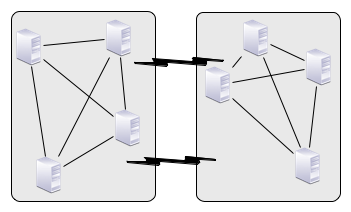
\includegraphics[width=\textwidth]{eps/no_queue}
        \caption{Without message queue}
        \label{fig_no_queue}
    \end{subfigure}
    ~ %add desired spacing between images, e. g. ~, \quad, \qquad, \hfill etc. 
      %(or a blank line to force the subfigure onto a new line)
    \begin{subfigure}[b]{0.32\textwidth}
        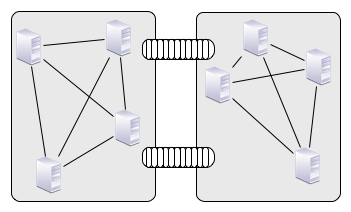
\includegraphics[width=\textwidth]{eps/yes_queue}
        \caption{With message queue}
        \label{fig_yes_queue}
    \end{subfigure}
    \begin{subfigure}[b]{0.32\textwidth}
        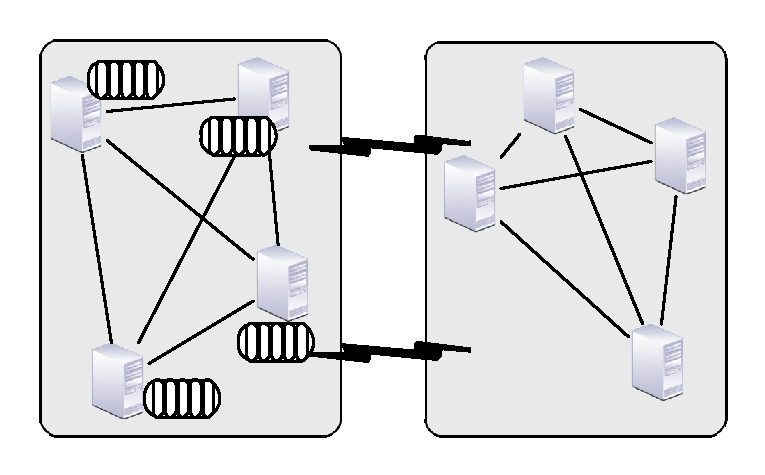
\includegraphics[width=\textwidth]{eps/node_queue}
        \caption{Partial message queue}
        \label{fig_partial_queue}
    \end{subfigure}
        \caption{Different system designs to connect data generator and SUT. \todo[inline]{O really do not get what the thunders represent and what this figure wants to present.}}
            \label{fig_queue_link}
\end{figure*}



\para{ \textit{Simplicity is key}}. The first challenge is to design a simple benchmarking framework as complex benchmarking frameworks can  cause  additional overheads. \todo[inline]{The number of components is not the only factor determining system complexity. Generally, I would prfer an argument on efficiency or low overhead than simplicity.=> deleted ambiguous part of sentence} \todo[inline]{AK: I really do not buy this argument of simplicity. Plus, "can cause additional overheads" without concrete reasons why, is very weak here.}

For example, the connection between the data generator and the SUT can cause large additional overheads when benchmarking.  To test the stream data processing engine, a data generator component is essential, to provide large amounts of streaming data. Figure \ref{fig_queue_link} shows  three possible cases to link the data generator and the SUT. The simplest design is to connect the SDPS directly to the data generators as shown in Figure \ref{fig_no_queue}. Although this is a perfectly acceptable design, it does not match real-life use-cases. In large-scale setups, stream data processing engines do not connect to push-based data sources but pull data from distributed message queues. A pull based design, where data sources and SUT are connected through queues, is in Figure \ref{fig_yes_queue}. A common bottleneck of this option is the throughput of the message queuing system. Also, this adds  a de-/serialization layer between the SUT and the data sources. Therefore, we use a third option, which is a hybrid of the first two. As can be seen in Figure \ref{fig_partial_queue}, we embed the queues as a separate module in the data generators. This way, the throughput is bounded only by the network bandwidth and the systems work more efficiently as there are no de-/serialization overheads.%\todo[inline]{not as simple as no queue...=>deleted sentence}


\para{ \textit{Separate driver and tested system}}. The second challenge is to isolate the  driver from the SUT as much as possible. In previous works, researchers measured the throughput  either  inside the SUT, or used internal statistics of the SUT. % or just do not mention about the measurement details. 
However, if the measurements and SUT are not separated, then the measurement computations can influence the results of benchmark.
In our benchmarking framework, we separate the driver and SUT for each measurement metric and perform measurements separately from the SUT. 
%\todo[inline]{I don't know what you want to say in this sentence. why would you associate the KPI/metric with a unit under test and what does that mean?-> I explained it in following sentences.}


The first metric is throughput. 
If the system can ingest and process all the data produced by the driver instances during the whole experiment, then the system can \textit{sustain} the given throughput and we call it \textit{sustainable throughput}. If the system sustains the given throughput and cannot process more, then we call it \textit{maximum sustainable throughput}. In this paper, we analyze the maximum sustainable throughput of SDPSs which is  sum of the throughputs of all driver instances. So, we keep throughput assessment inside driver instances and sum them at the end of experiment. 

\todo[inline]{AK: Please explain the throughot concept better or refer to where in the paper this is explained.}

  
The second evaluation is latency. We define the latency of a tuple to be the interval between tuple's event time and emission time from SUT's sink operator. We develop a model to calculate the latency of stateful operator  which we analyze in Section \ref{sec_latency}.
%\todo[inline]{I like the concept of isolating the driver, however, separating would be a better term. But the description of this separation is completely unclear. Also, if it is required to separate, you should explain why and how we did it. You have some of the why but none of the how=>fixed}

\para{ \textit{Unreal latency and throughout}}.
The third challenge is to measure the metrics with close to real-life scenarios. %\todo[inline]{This is repetitive, you need to mention real world only once in this paragraph=>fixed} 
One example  is the throughput measurement. In the previous SDPS benchmarks, the throughput of a SUT is measured by either taking quantiles over the test duration, or showing max, min, and average results. 
%\todo[inline]{Why? And what do you mean by reason about the SUT. This sentence needs to be rewritten => deleted sentence}
From a user's perspective on the other hand, the system's throughput is the upper limit throughput that it can sustain in a realistic setup. 
We propose user-defined sustainability policies in our benchmarking framework. For example, the benchmarking framework can take into account the backpressure of  the SUT.  %\todo[inline]{Again repetitive and convoluted, make the text simple and say right away what you want to say instead of incrementally adding parts=>fixed}

\todo[inline]{AK: I really don't get what unreal throughput is and why we use this term. I did not see it anywhere else so far.}


Another example for this challenge is latency measurement. If there are additional systems between the SDPS and data source (driver), then those are likely to add an extra latency for each tuple.  One solution is  to measure the latency in the SDPS the same way as it is measured in batch data processing systems. In this case, the number and complexity of the systems between SDPS and data source is irrelevant as the latency is the interval between tuples' ingestion and output from SUT. However, this measurement of latency is too \textit{optimistic} and does not result in the real latency of the tuple. The reason is that  the actual latency is based on tuples' event generation time. For example in online games, the event time can be a user's specific action in a game, the latency then is the time interval between user's action and the result being emitted from the SDPS. Therefore, the usual method of measuring the latency within SDPS does not conform to real world scenarios especially in pull-based SDPSs. Depending on their backpressure mechanism, a pull-based SDPS will reduce the input rate on high loads, which will not be reflected in the measured latency. To solve this, we define the latency for SDPSs to be the difference between tuple's event time and output time. 

Another factor triggering the unrealistic latency is the data generation rate. If the input data rate is higher than the SDPS's \textit{maximum sustainable throughput} and we measure the event time latency, the results may not exhibit the real  latency. 
Initially the system will try to ingest as much data as possible. As a result, the SUT's processing time will take longer and the latency will increase for every adjacent tuple. To solve this issue, we conduct experiments with the maximum sustainable throughput for each SDPS. 
%\todo[inline]{The previous text is confusing. Try to make it simple and precise}
%\todo[inline]{What does associate mean?->deleted}
%\todo[inline]{Repetition=>fixed}
%\todo[inline]{This means we do not measure system latency? Then this is a component benchmark and cannot report on application level performance. This is also contradictory to previous discussions about the separation of driver and sut=>rewritten above}
%\todo[inline]{I think this was written several times already.=>rewritten above}   \todo[inline]{Again, repetition. Please concentrate on the message this section is supposed to convey. This would be the challenge of measuring latency. I have not clearly read your solution to the problem.=>rewritten above}


\para{ \textit{Latency of stateful operators}} The final challenge is measuring the latency of stateful operators. Up to this point, the related work either concentrated on stateless operators or evaluated the latency of stateful operators by checkpointing to external systems. As we discussed above, this approach can be a bottleneck and will influence the measurements. In our benchmarking framework, we propose a solution to this problem.  
We aggregate tuples by selecting their maximum timestamp and append the resulting timestamp to the emitted tuple from stateful operator. 
 In this way, we measure the latency of stateful computation time, excluding the tuples' waiting time (in window) in stateful operator. 

%\todo[inline]{Did we remove the formal definition, then this should be updated=>fixed}


\section{Benchmark system design}
\label{des}
We keep overall design of benchmark simple. Figure \ref{fig_design} shows the overall intuition behind the benchmark system. There are two main components of a system: \textit{i)} SUT and \textit{ii)} Data Engine. Data Engine has 2 subcomponents being \textit{i)} Data Generator and \textit{ii)} Data Queue.

The Data Engine component is responsible for generating and queueing the data. Both of its subcomponents reside in the same machine to avoid network overhead and to ensure the data locality. The data is kept in memory to circumvent the disk write/read overhead. First subcomponent, Data Generator, generates data with a given speed. The speed is constant throughout the benchmark.  To ensure high throughput we keep the number of fields in an event minimal. To assure the data locality  each Data Generator connects to Data Queue residing in the same machine. Because of the bottlenecks explained in Section \ref{chal}, we avoid queueing data in  centralized message queues. Queues in Data Queue subcomponent are based on FIFO semantics. Theoretically, this approach has no difference from implementing the  centralized and distributed message queues between SUT and data source. The following analogy can be made: the topic in distributed message queueing system is analogous to set of all Data Queues, and partition is the single Data Queue. The Data Generator appends the current time to timestamp field of an event. The event's latency is calculated from this point and the more it stays in queue, the more the latency is. The number of Data Engines can be arbitrary and its overall throughput is only bounded by network bandwidth. As we discussed above, the throughput assessment which is associated with the SUT as a whole,  is done in Data Engine component, which has a clear separation from SUT. 

The SUT is another component of a system, which processes the data.  Because the only interface of Data Engine to outer world is Data Queue subcomponent,  SUT pulls data from Data Queue. The connection is pull based because we let the SUT to decide the frequency of data ingestion. The SUT connects predefined number of Data Queues. The pulled data from multiple Data Queues is combines inside SUT. There can be one or two unions, depending on the operator semantics. For example, windowed aggregation is a single input stream operator but join operator accepts two streams  as an input. So, for windowed aggregation operator we union all input streams and give as an input. On the other hand, for windowed join operator, we make two unions of input streams and give them as an input.  The latency calculation is done inside SUT. This measurement is associated with the operator inside SDPS, we clearly separate the latency assessment from Operator Under Test (OUT). Placing extra stateless operator just after OUT and measuring the latency between the event time and current time gives the latency of an element. The calculation of latency in windowed aggregation and windowed join operators is shown in Section \ref{sec_latency}. 


%Proper handling tuples' timestamp fields while joining or aggregating is crucial. In this work, \textit{merging} of tuples' timestamp fields is done by selecting \textit{maximum} over them. That is, latest arrived tuple's timestamp is transferred to the new tuple as a result of aggregation or join. Equation \ref{eq_1} defines this logic formally.
%
%
%Here $t \in T$ is a stream tuple,  $t[k]$ is  $k^{th}$ field of particular data point and $\equiv$ means equivalent in terms of type. For aggregation function $|T|$, the size of a set is not bounded, whereas for join function it is bounded by two, being $|T| = 2$.

\begin{figure*}[h]
\centering
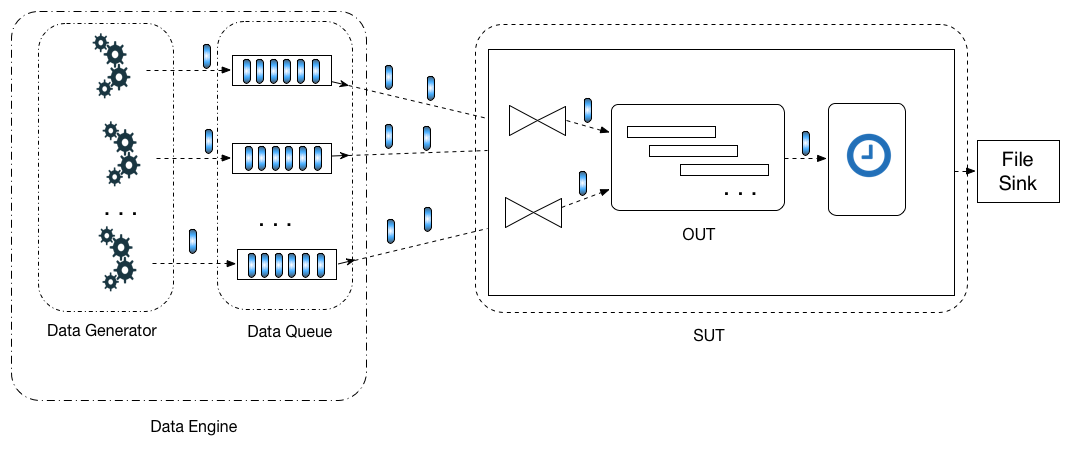
\includegraphics[width=1\textwidth]{eps/system_design}
\caption{Design of benchmark system.}
\label{fig_design}
\end{figure*}

\subsection{Use case}
The use case for this benchmark is provided by \textit{ Rovio Entertainment}. It is known as a video game development company. To get higher customer satisfaction, it is mandatory to analyse the game usage statistics. For example, company releases a new feature for a particular video game. It is essential to have a quick overview of customer's opinion by analysing the usage statistics. For that reason, Rovio uses stream data processing analytics rather than batch based periodic analysis.  In all use cases an event has following fields: event timestamp, key and value. 

\textbf{Windowed Aggregation}
Windowed aggregations are important part of the statistics analytics from the feed stream. One use case is computing the user average session time within windows. Each event has its geo ID, which indicate the location in which an event was generated. A use case includes partitioning the events by their ID and finding the average session time within windows. Here, the key field is geo location and value field is session time. Another use case is computing the average ads screening time within window for each geo location. 

\textbf{Windowed Join}
Joining several stream feeds based on key field within window is another general use case for user statistics analytics. One specific use case is joining two user statistics stream feed within window by geo field and calculating an event with higher session time and the difference between them. In this use case the key field would be geo location and value would be the session time. Another use case would be doing the same procedure with ads watch time. 


\subsection{Key Performance Indicators}
The Key Performance Indicators ( KPIs) for this benchmark are latency and throughput. The throughput indicator is related with SUT, on the other hand, the latency is associated with OUT. 


%To measure the performance of a system, we connected max $16$ data generators to system under test with order of $1$,$2$,$4$,$8$ and $16$ as increasing further does not increase the overall throughput significantly. We call the tests with related workloads as $1x$, $2x$, $4x$, $8x$ and $16x$. Moreover, the configuration of each data generator must be the same. Configuration includes parameters such as overall input size, generation speed, socket port and etc. Equation \ref{eq_2} defines this formally.
%
%\begin{equation}
%  \begin{gathered}
% \textbf{Let} \ d_{i}^{c_{i}} \in  D\\
%  \textbf{then}, |D| \gets S \\
%  \textbf{and} \ c_{1} = c_{2} \ ... = c_{n}, \forall n \in S = {1,2,4,8,16}
%  \end{gathered}\label{eq_2}
%\end{equation}


\subsubsection{Throughput}
\textit{Definition.  Let $c_{i} \in C$ be a configuration for a Data Engine, $d_{i} \in D$,  $c_{i}^{sp}$ be the data generation speed configuration which can be sustained by SUT. If  $\exists c_{i} \in C$ such that $c_{1} = c_{2}... = c_{i}$ and  $T = \sum_{i}c_{i}^{s}$ is maximum, $\forall c_{i} \in C, \forall i \in \{1,2,3 ... |C|\}$, then $T$ is a maximum sustainable throughput of SUT.}

Throughput of a system is calculated as summing the throughout of each Data Engine  because the SUT is expected to pull the data from all Data Queue subcomponent of Data Engine approximately with same rate. We restricted the configuration of all Data Engines to be the same, to ease calculating the maximum sustainable throughput. It is crucial to note that the maximum sustainable throughput is not the same as maximum throughput of Data Engine but the one for SUT. 

To examine the system's sustainability with a given throughput, we divide the queue used in Data Queue subcomponent into three parts: $c^{a}$ , $c^{b}$ and $c^{n}$. The Figure \ref{fig_queue}, shows the example partitioning of queue. If the size of the queue is less than or equal to $c^{a}$ then this is acceptable and means, the SUT can sustain the given throughput. If the queue size is less than or equal to $c^{b}$ on the other hand, the SUT cannot sustain the given data rate but we can tolerate it for some time, in case the increase in queue size is an outcome of back-pressure. However, if the queue size is bigger than the $c^{b}$ then the SUT cannot sustain the given throughput and there is no need to do benchmarks with particular data rate.

The semantics behind  examination of SUT's sustainability with a given throughput must be clear. Moreover, it should support the system specific behaviours like back-pressure. Algorithm \ref{alg_sustainable} show an algorithm to check if the  SUT can sustain  the given throughput of a single Data Engine. It gets the configuration $c$ of Data Engine as an input. After firing the Data Engine with configuration $c$, in line $3$, it is put to $idle$ position, meaning no data is generated until the SUT makes its first data pull request from Data Queue subcomponent. $c^{input}$ is the input count that must be generated in particular Data Engine.
 In lines $10-11$ the events are generated with speed $c^{sp}$ in Data Generator subcomponent of Data Engine component and put into the queue of Data Queue subcomponent. We check the queue size periodically, once per $c^{a}$ element and not for each iteration. The first reason is that the data pull rate of stream data processing engine is not steady and therefore checking the queue size with little delays makes more sense. The second reason is that, $c^{a}$ can be thought of the $confidence limit$ as shown in Figure \ref{fig_queue}. While checking the queue size there are three possibilities. The first is (lines $13-15$), the size is bigger than $c^{b}$, the back-pressure limit. In this case, the Data Engine is stopped and the $false$ is returned meaning the SUT is not sustainable with given throughput. The second is (lines $16-18$), queue size is less than $c^{a}$, the acceptable queue size. In this case, we set back-pressure counter to zero, in case there was one and continue generating data. The third is (lines $19-23$), the size   of queue is within boundaries of $c^{a}$ and $c^{b}$. In this case, we can tolerate the SUT for at most $\frac{c^{b}}{c^{a}}$ times. If the system can pull the data in queue and set the size of queue within \textit{confidence} boundaries ($c^{a}$) in a given period, then it continues, else, the application returns $false$ meaning, the SUT cannot sustain the given throughput. 

\begin{algorithm}
    \SetKwInOut{Input}{Input}
    \SetKwInOut{Output}{Output}

    \underline{function isSustainable} $(c)$\;
    \Input{ $c$ is configuration of Data Engine}
    \Output{return $true$ if is sustainable, $false$ otherwise}
    Fire Data Engines with configuration $c$. \\
    $c^{st} \gets idle$  \tcp*{wait for SUT to pull data}
  \While{There is no pull request from SUT}{
    wait \\ 
   }    
       $c^{st} \gets active$ \tcp*{start generating data}
       $bp\_index \gets 0$ \tcp*{initialize back-pressure index}
       \For{$i \gets 0; i < c^{input}; i++$}{
       Generate $e_{i} \in E$ with speed $c^{sp}$\\
       queue.put($e_{i}$) \tcp*{put  generated event to queue}
        \tcc{check the queue once per $c^{a}$ elements}
        \uIf{i \% $c^{a} == 0$}   { 
               \uIf{ $queue.size > c^{b}$  }   { 
              		Stop Data Engine \\
		         return $false$
               }
               \uElseIf{  $queue.size < c^{a}$ }{
               $bp\_index \gets 0$ \tcp*{ no back-pressure} 
               $continue$ \tcp*{SUT can sustain so far} 
               }
               \uElse{ 
                \tcc{ Tolerate for back-pressure}
                  $bp\_index \gets bp\_index +1$ \\
                     \uIf{$bp\_index == \frac{c^{b}}{c^{a}}$}{
                       \tcc{ This is not back-pressure}
                        Stop Data Engine \\
		         return $false$  
                     }
               }
        }
       }
    \caption{Throughput sustainability test of single data engine}
    \label{alg_sustainable}
\end{algorithm}

\textit{Definition.  Let $c_{i} \in C$ be a configuration for a Data Engine, $c_{i}^{dr}$ be a data generation rate of particular Data Generator, $d_{i} \in D$ and $n$ be the number of Data Engines being $n = |D|$.  The SUT is sustainable with given throughput $n * c_{dr}$,  $iff$ $isSustainable(c_{i})  == true$ $\forall$ $i \in \{1,2,3,...n\}$}

The above definition states that the SUT is sustainable with a given data generation rate iff, it can sustain all Data Engines at the same time. If one of the Data Engines cannot be sustained, then SUT is said is not sustainable with a given data generation rate. 


\subsubsection{Latency}
\label{sec_latency}
Latency is another KPI for this benchmark and defining the latency needs clear semantics. There are several points that needs to be clarified: \textit{i)} the aggregation or join of timestamp fields of tuples and \textit{ii)} clear boundaries (start and end timestamp) of latency.

The first point is the aggregation or join of tuples with timestamp fields. While the use case provides the semantics for aggregating or joining the tuples' $value$ fields, the one for timestamp field is unclear. For example, in windowed aggregation operator, which calculates the average of elements' $value$ field, the aggregation semantics with tuples' timestamp field is unclear.  The Equation \ref{eq_1} addresses this issue. Let $t[k]$ and $t'[k]$ denote the timestamp field for tuples $t$ and $t'$ respectively,  $\equiv$ be an operator checking for the type and $TS$ be tuple field of type timestamp. Here, $f_{s}$ is an stateful operator which takes a set of tuples $t \in T$ and converts it to tuple $t'$. Then there exists $k$ and $m$ such that the respective fields of input and output tuples have the same type being timestamp and the output tuple's timestamp is calculated taking maximum among input tuples. Here input and output tuples are associated with operator $f_{s}$ and not with the SUT.

To calculate the latency, it is crucial to have clear boundaries of when to start and stop the stopwatch for each tuple. Equation \ref{eq_2} defines the basic semantics behind this. This is basically a follow-up for Equation \ref{eq_1}. Let $t_{i} \in I$ be a tuple in input set and $t_{o} \in O$ be a tuple in output set. The latency is associated with output tuples. So, the latency of tuple $t_{o}$ is calculated by extracting the $t_{o}[m]$, the timestamps field from current time. The calculation of output tuples' timestamp field is shown in Equation \ref{eq_1}. 


\begin{equation}
  \begin{gathered}
\textbf{Let} f_{s}:\{t| t\in T \} \to t'  , \\
  \textbf{then}, \exists k,m \ s.t. \ t[k]  \equiv t'[m] \equiv \ TS \ \forall t \in T\\
  \textbf{and} \ t'[m] \gets \argmax\{t[k] \ | \ t \in T\}  
    \end{gathered}
      \label{eq_1} 
  \end{equation}

   \begin{equation}
     \begin{gathered}
  \textbf{Let} \ t_{i} \in I , t_{o} \in O \\
\textbf{then} \ Latency_{ \ t_{o}} = time_{now} -  t_{o}[m] \\
s.t. \ f_{s}:\{t_{i} \ | t_{i} \in I \} \to \{t_{o} \ | t_{o} \in O \} \\
\textbf{and} \ t_{o}[m] \equiv TS
  \end{gathered}
  \label{eq_2} 
\end{equation}



\begin{figure}[h]
\centering
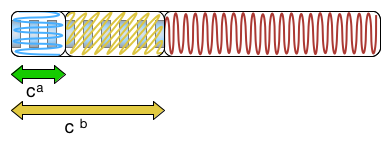
\includegraphics[width=0.7\textwidth]{eps/queue}
\caption{Basic intuition behind \textit{back-pressure-compatible queue}}
\label{fig_queue}
\end{figure}

\begin{figure}[h]
\centering
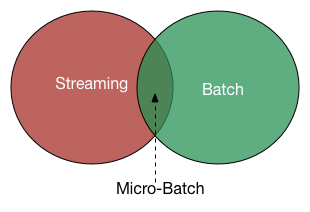
\includegraphics[width=0.35\textwidth]{eps/streambatch}
\caption{Conceptual view of micro-batching}
\label{fig_micro_batch}
\end{figure}







\section{Evaluation}
\subsection{Configuration}
The following configurations are used throughput experiments:
\begin{itemize}
\item Cluster size: 2,3,4 and 8 node clusters
\item Parallelism within single node: number of cores, which is 16.
\item Parallelism within cluster: (Parallelism within single node) * (number of nodes)

\item Backpressure: enabled in all systems
\item Network bandwidth: 1Gb
\item Number of Data Engines running in parallel: 16
\item Allocated memory: 16GB
\item Cluster type: Standalone
\item Input size for aggregation use case: 150M * 16
\item Input size for join use case: 
\item Spark batch size: 4 seconds and 2 seconds
\item Window type: Processing time
\item Number of distinct keys in input: 160
\item Join inputs selectivity: 
\item $c_{a}$, acceptable queue limit: 1M
\item $c_{b}$ backpressure tolerated queue limit: 15M
\end{itemize}

\subsection{Keyed Windowed Aggregations}

\subsubsection{Storm}


\begin{figure*}
    \centering
    \begin{subfigure}[b]{0.49\textwidth}
        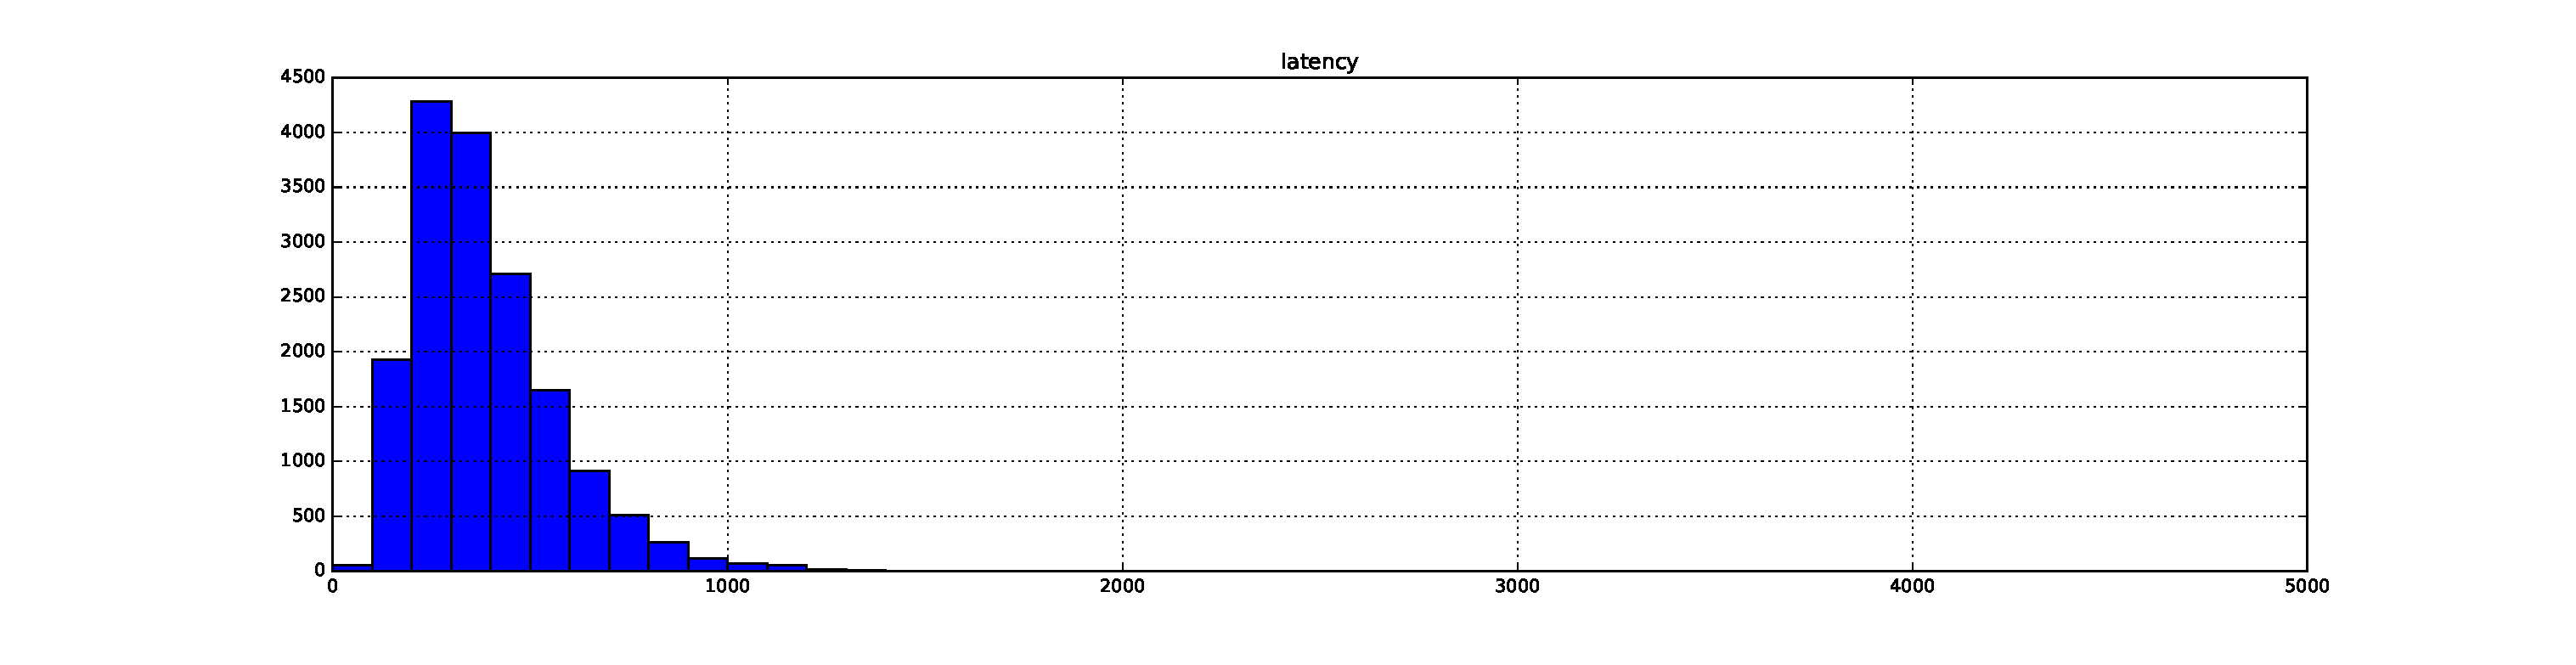
\includegraphics[width=\textwidth]{storm/2_1}
        \caption{2 Node latency histogram}
        \label{fig_no_queue}
    \end{subfigure}
    ~ %add desired spacing between images, e. g. ~, \quad, \qquad, \hfill etc. 
      %(or a blank line to force the subfigure onto a new line)
    \begin{subfigure}[b]{0.49\textwidth}
        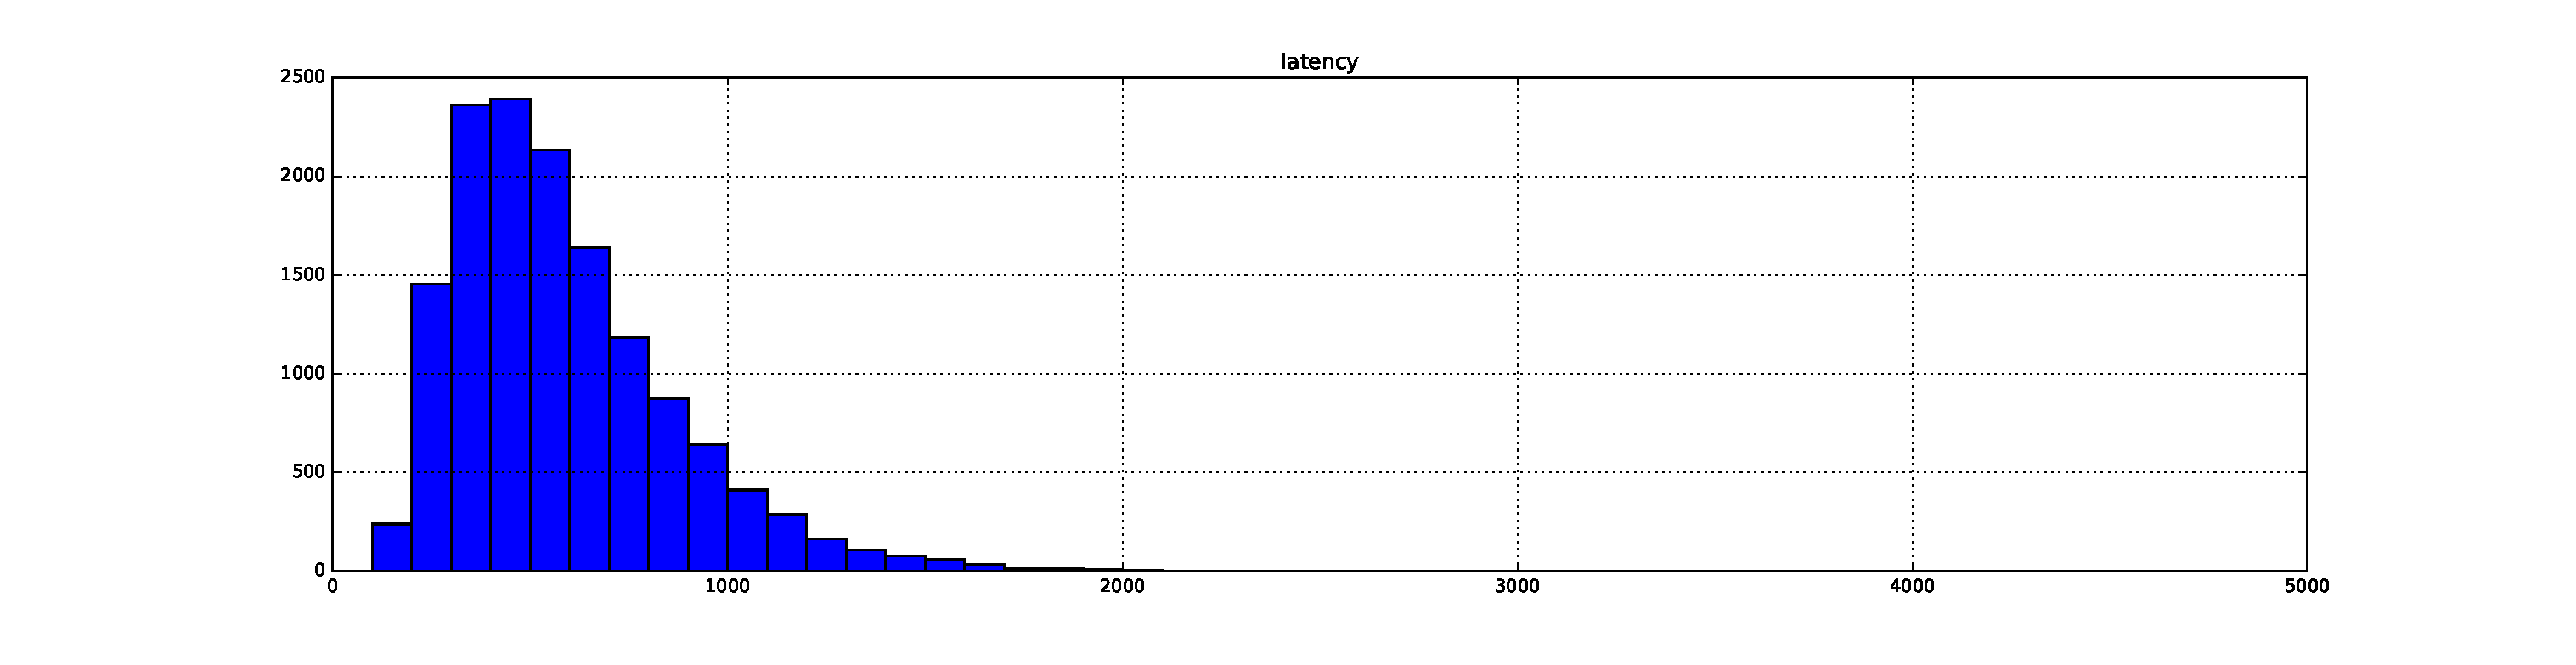
\includegraphics[width=\textwidth]{storm/3_1}
        \caption{3 Node latency histogram}
        \label{fig_yes_queue}
    \end{subfigure}
    ~ %add desired spacing between images, e. g. ~, \quad, \qquad, \hfill etc. 
    %(or a blank line to force the subfigure onto a new line)
    \begin{subfigure}[b]{0.49\textwidth}
        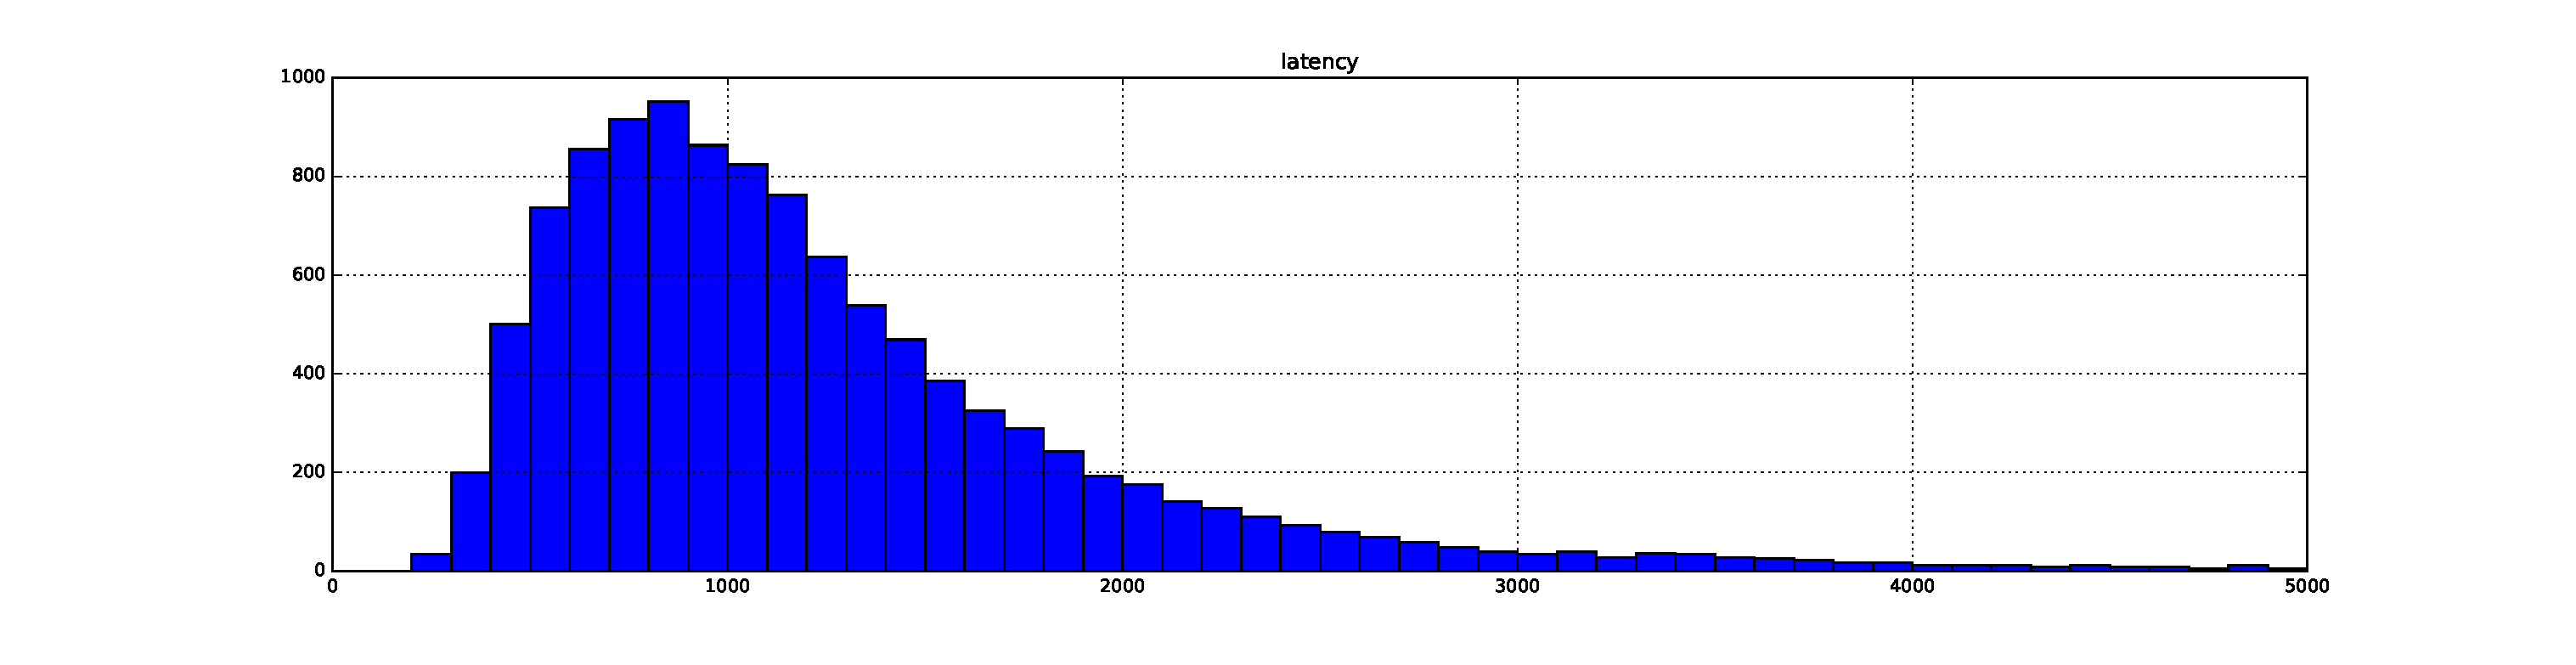
\includegraphics[width=\textwidth]{storm/4_1}
        \caption{4 Node latency histogram}
        \label{fig_partial_queue}
    \end{subfigure}
        \begin{subfigure}[b]{0.49\textwidth}
        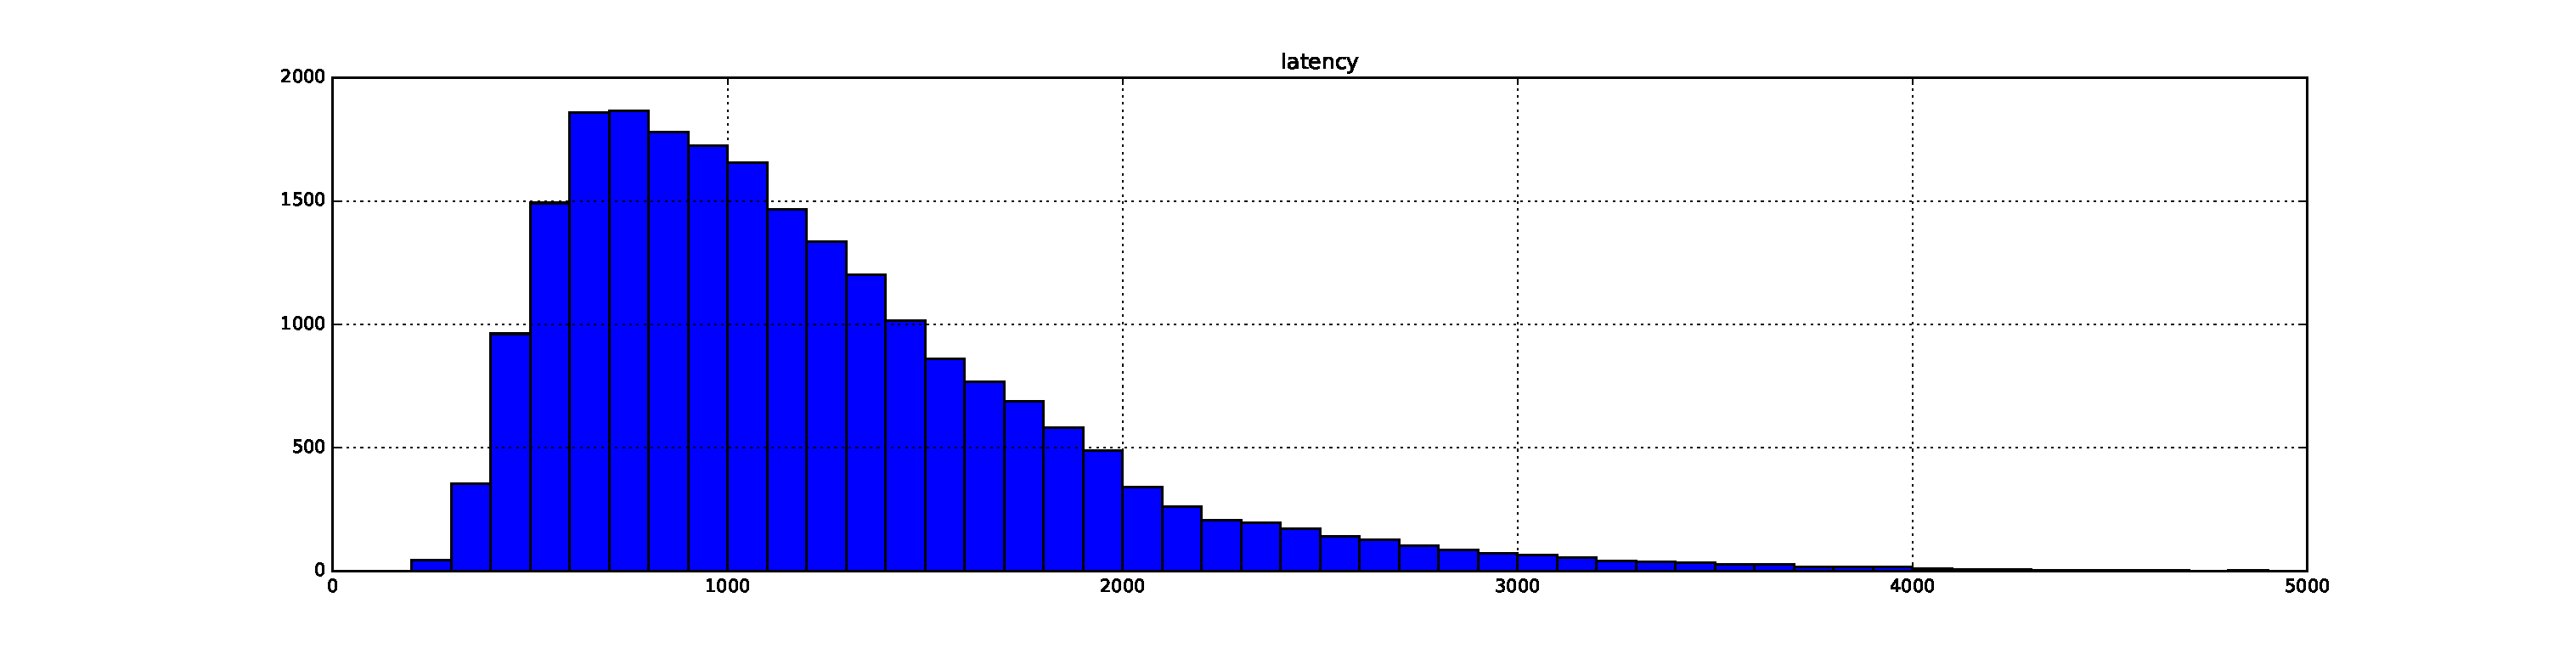
\includegraphics[width=\textwidth]{storm/8_1}
        \caption{8 Node latency histogram}
        \label{fig_partial_queue}
    \end{subfigure}


    \begin{subfigure}[b]{0.49\textwidth}
        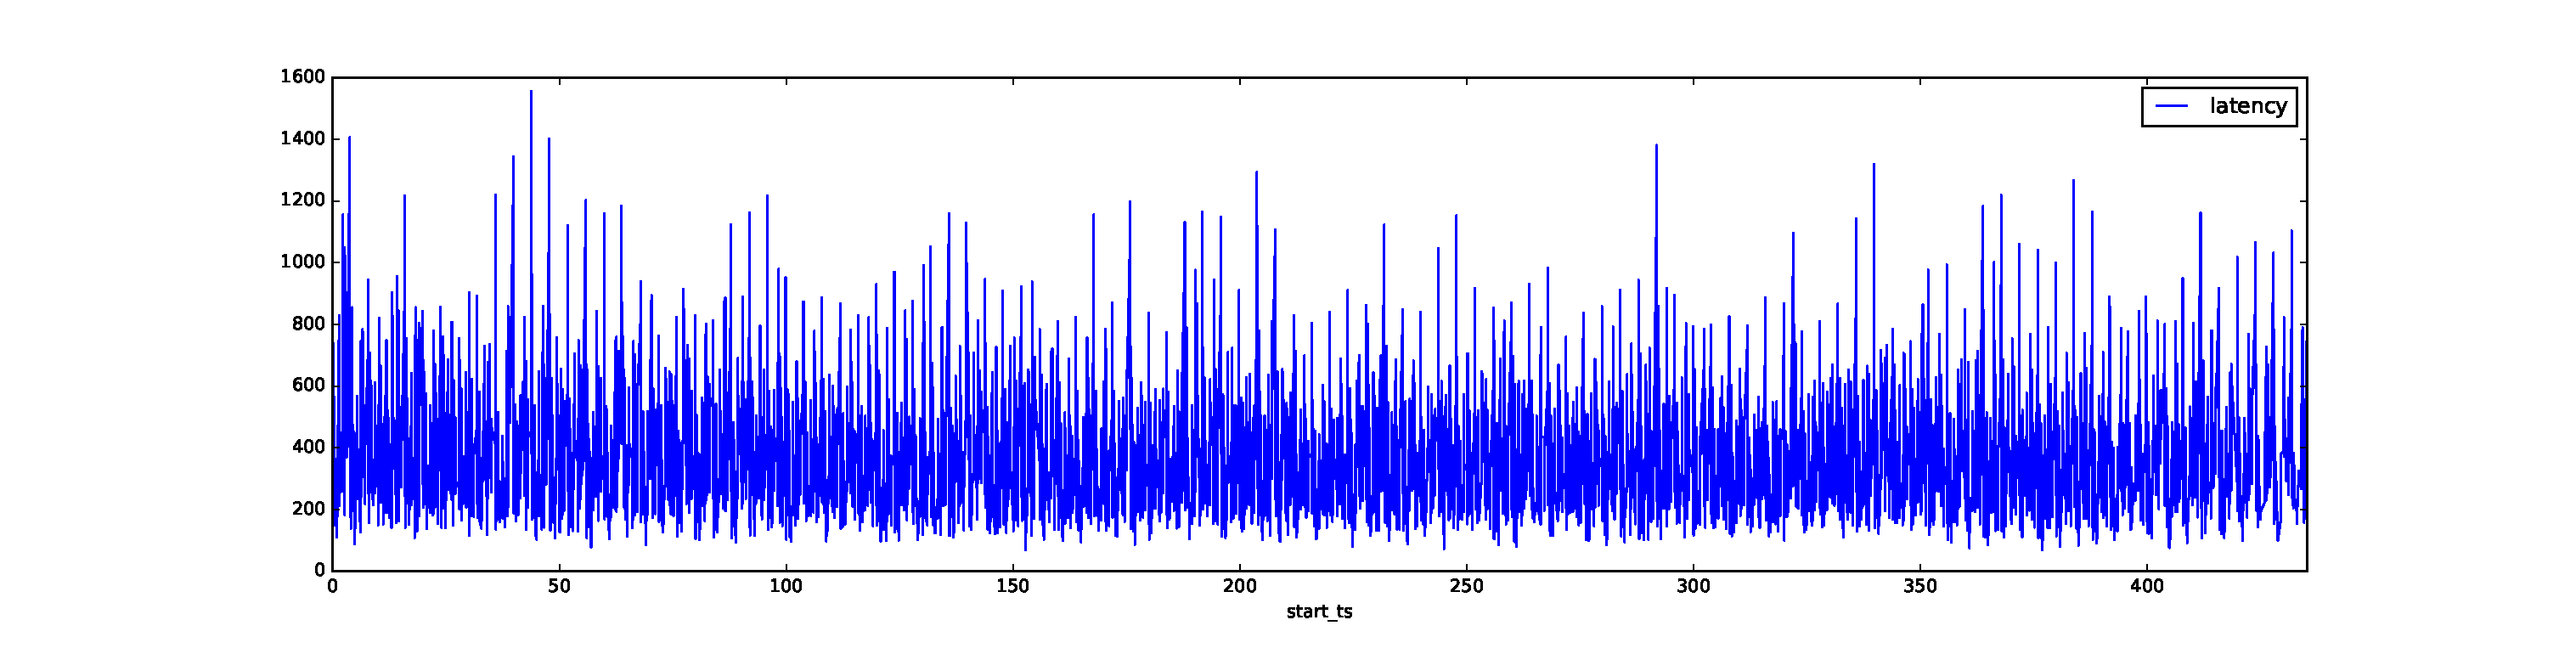
\includegraphics[width=\textwidth]{storm/2_2}
        \caption{2 Node latency time series}
        \label{fig_no_queue}
    \end{subfigure}
    ~ %add desired spacing between images, e. g. ~, \quad, \qquad, \hfill etc. 
      %(or a blank line to force the subfigure onto a new line)
    \begin{subfigure}[b]{0.49\textwidth}
        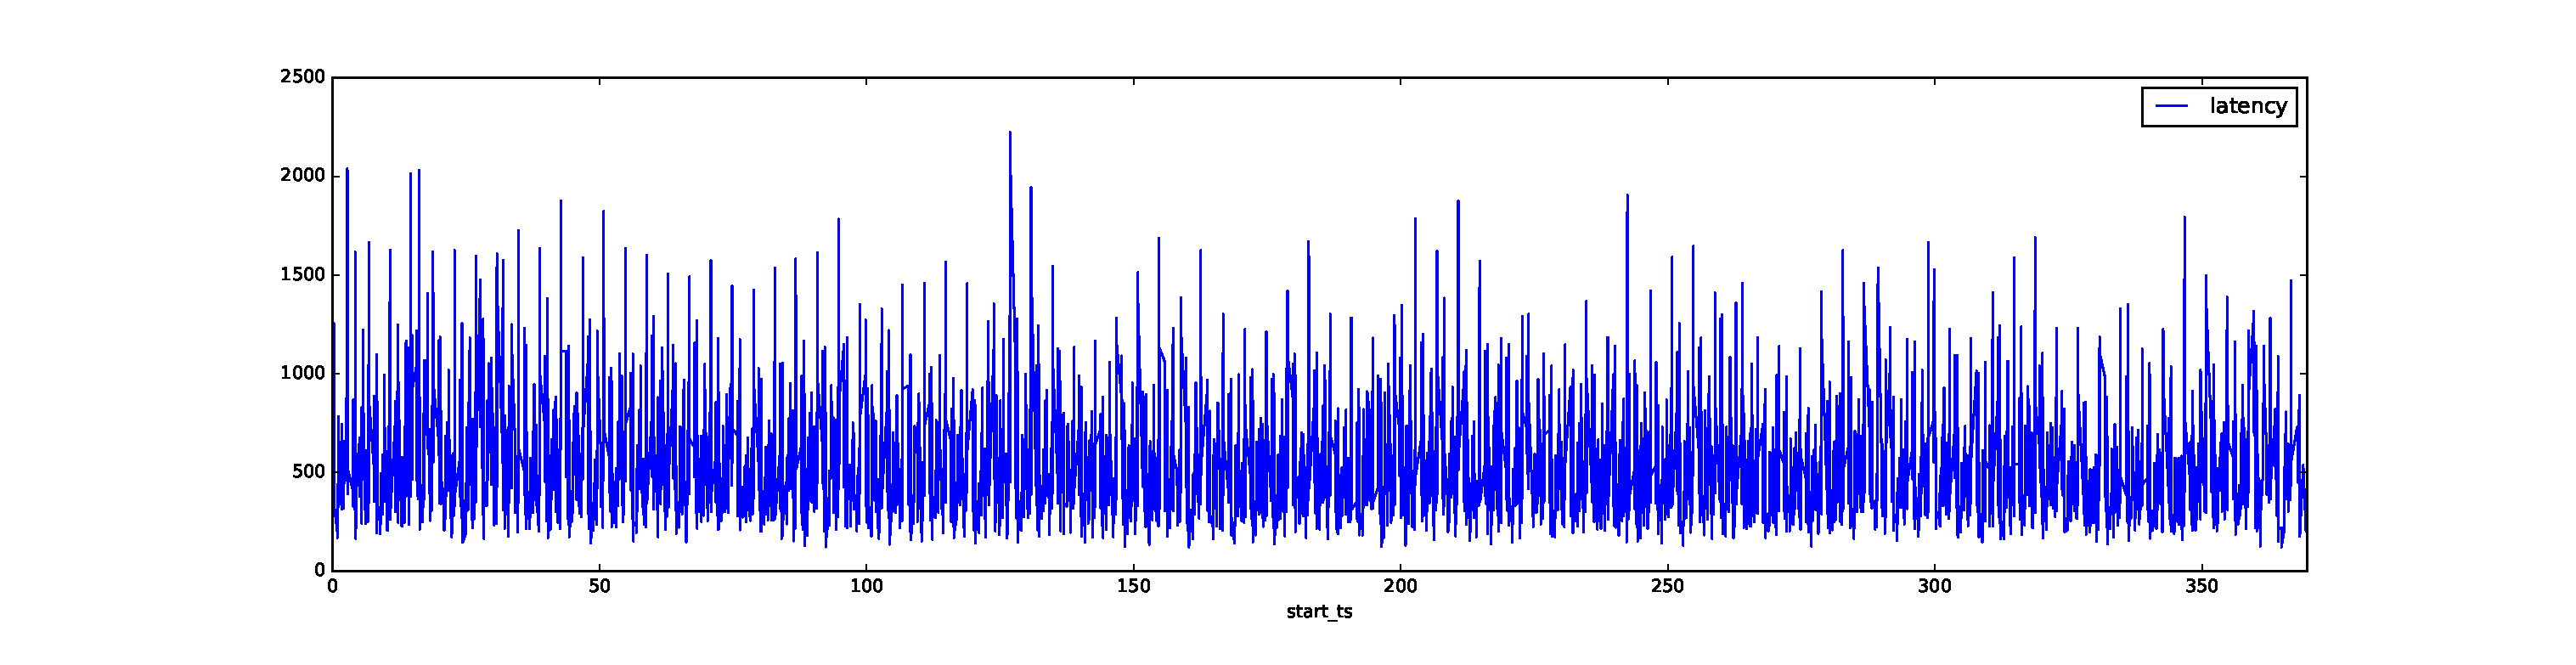
\includegraphics[width=\textwidth]{storm/3_2}
        \caption{3 Node latency time series}
        \label{fig_yes_queue}
    \end{subfigure}
    ~ %add desired spacing between images, e. g. ~, \quad, \qquad, \hfill etc. 
    %(or a blank line to force the subfigure onto a new line)
    \begin{subfigure}[b]{0.49\textwidth}
        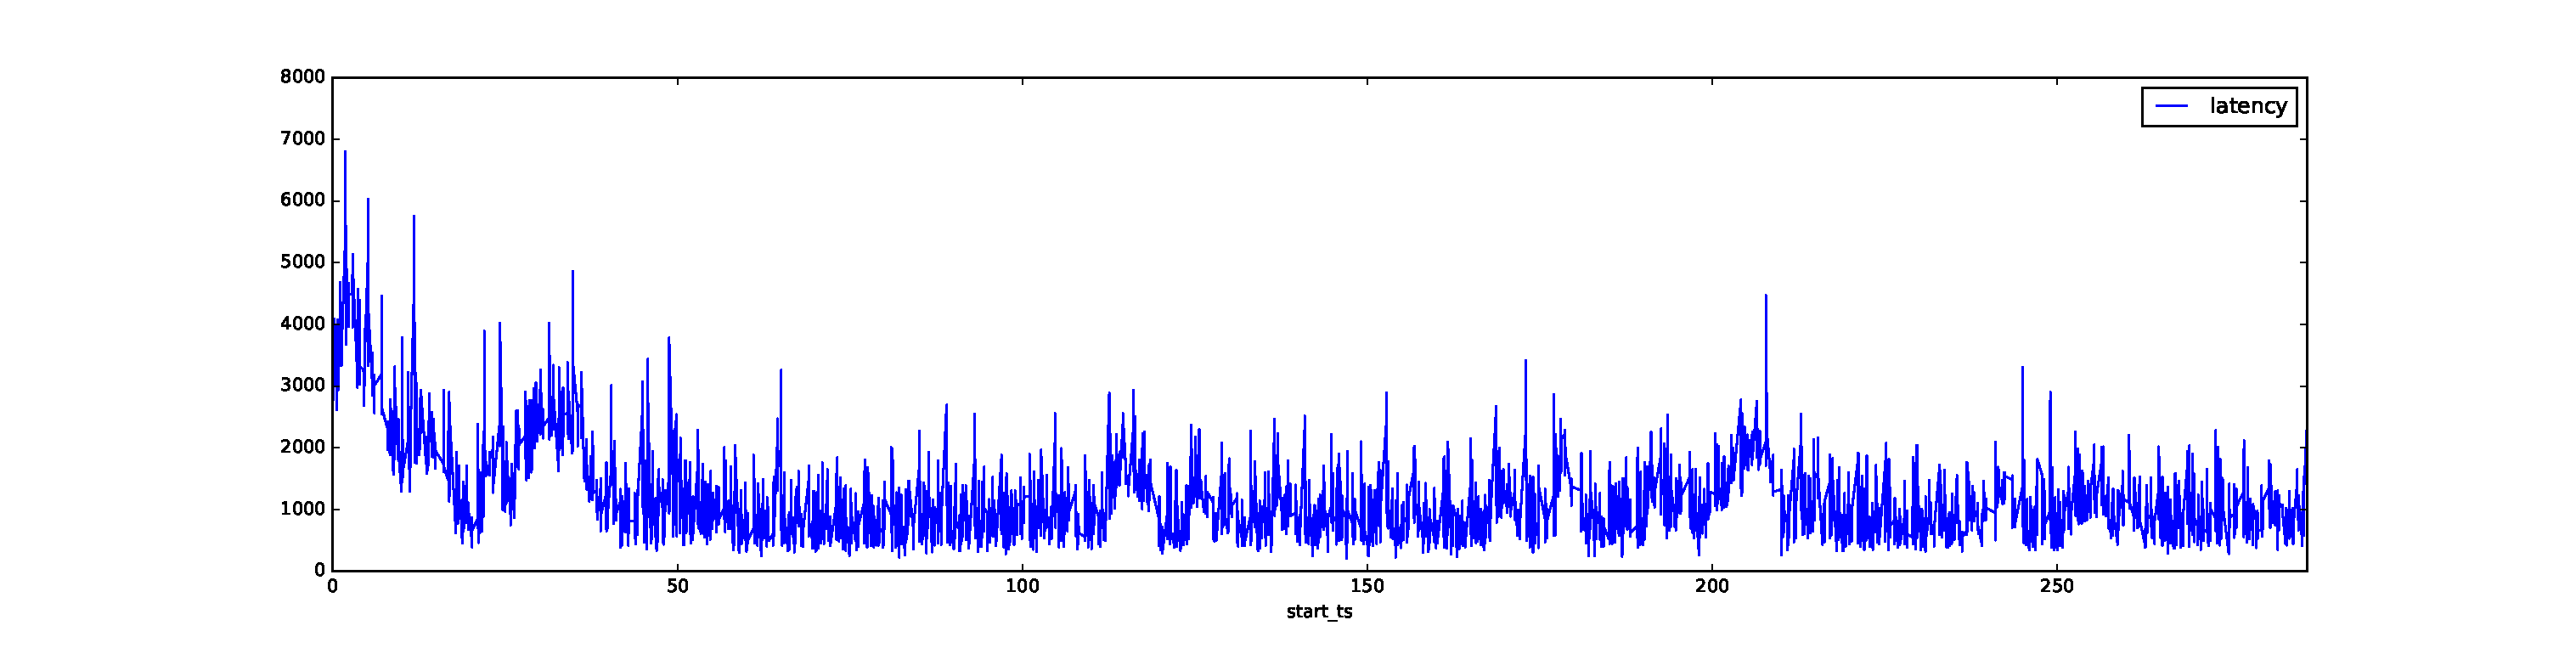
\includegraphics[width=\textwidth]{storm/4_2}
        \caption{4 Node latency time series}
        \label{fig_partial_queue}
    \end{subfigure}
        \begin{subfigure}[b]{0.49\textwidth}
        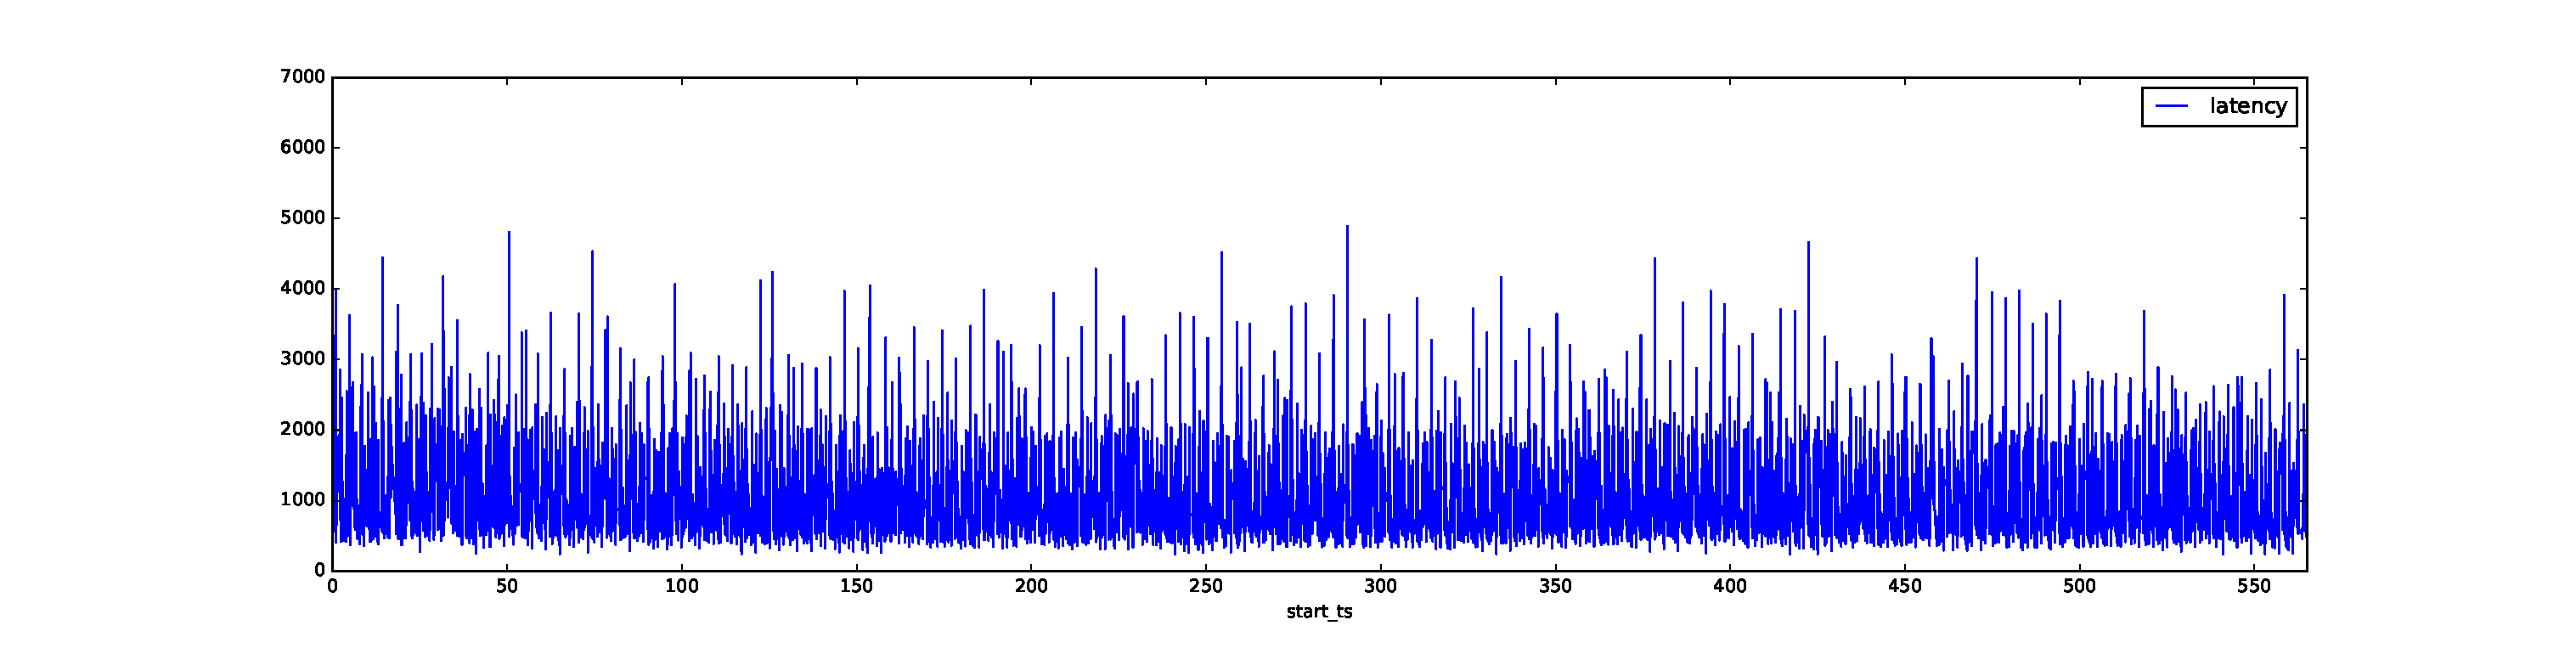
\includegraphics[width=\textwidth]{storm/8_2}
        \caption{8 Node latency time series}
        \label{fig_partial_queue}
    \end{subfigure}

    \label{fig_flink_agg_1}
        \caption{Latency of windowed aggregations for Storm}
\end{figure*}


\subsubsection{Spark}



\begin{figure*}
    \centering
    \begin{subfigure}[b]{0.49\textwidth}
        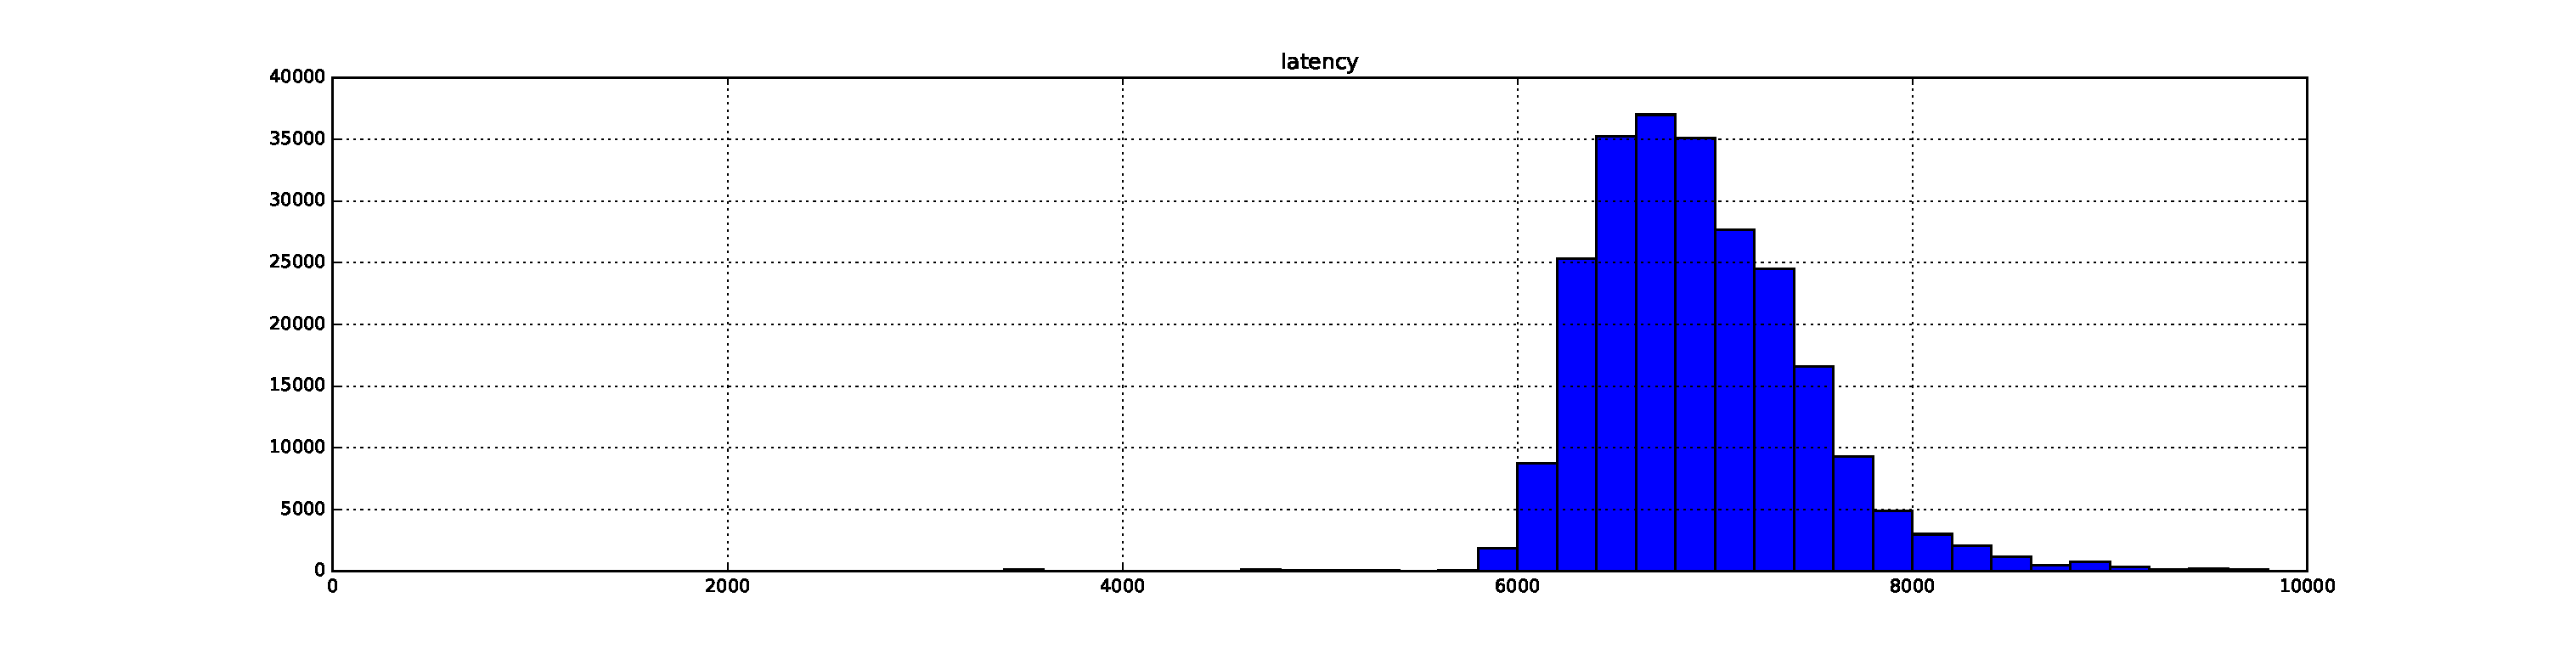
\includegraphics[width=\textwidth]{spark/2_4_1}
        \caption{2 Node latency histogram}
        \label{fig_no_queue}
    \end{subfigure}
    ~ %add desired spacing between images, e. g. ~, \quad, \qquad, \hfill etc. 
      %(or a blank line to force the subfigure onto a new line)
    \begin{subfigure}[b]{0.49\textwidth}
        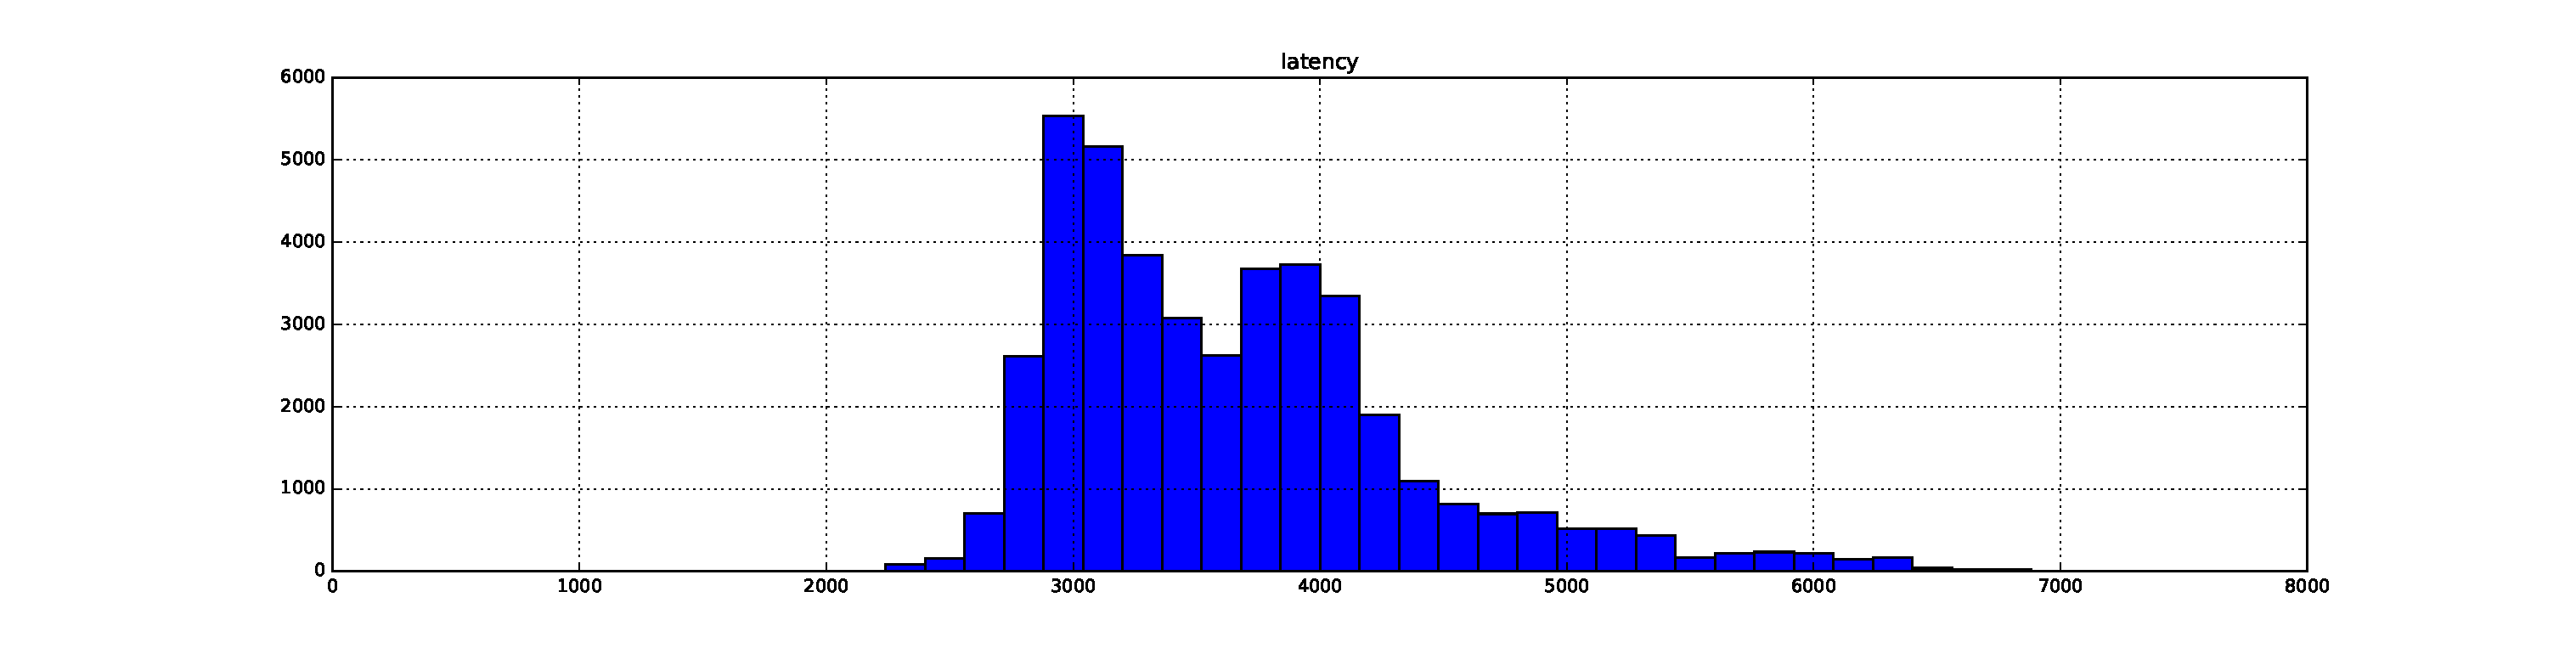
\includegraphics[width=\textwidth]{spark/3_4_1}
        \caption{3 Node latency histogram}
        \label{fig_yes_queue}
    \end{subfigure}
    ~ %add desired spacing between images, e. g. ~, \quad, \qquad, \hfill etc. 
    %(or a blank line to force the subfigure onto a new line)
    \begin{subfigure}[b]{0.49\textwidth}
        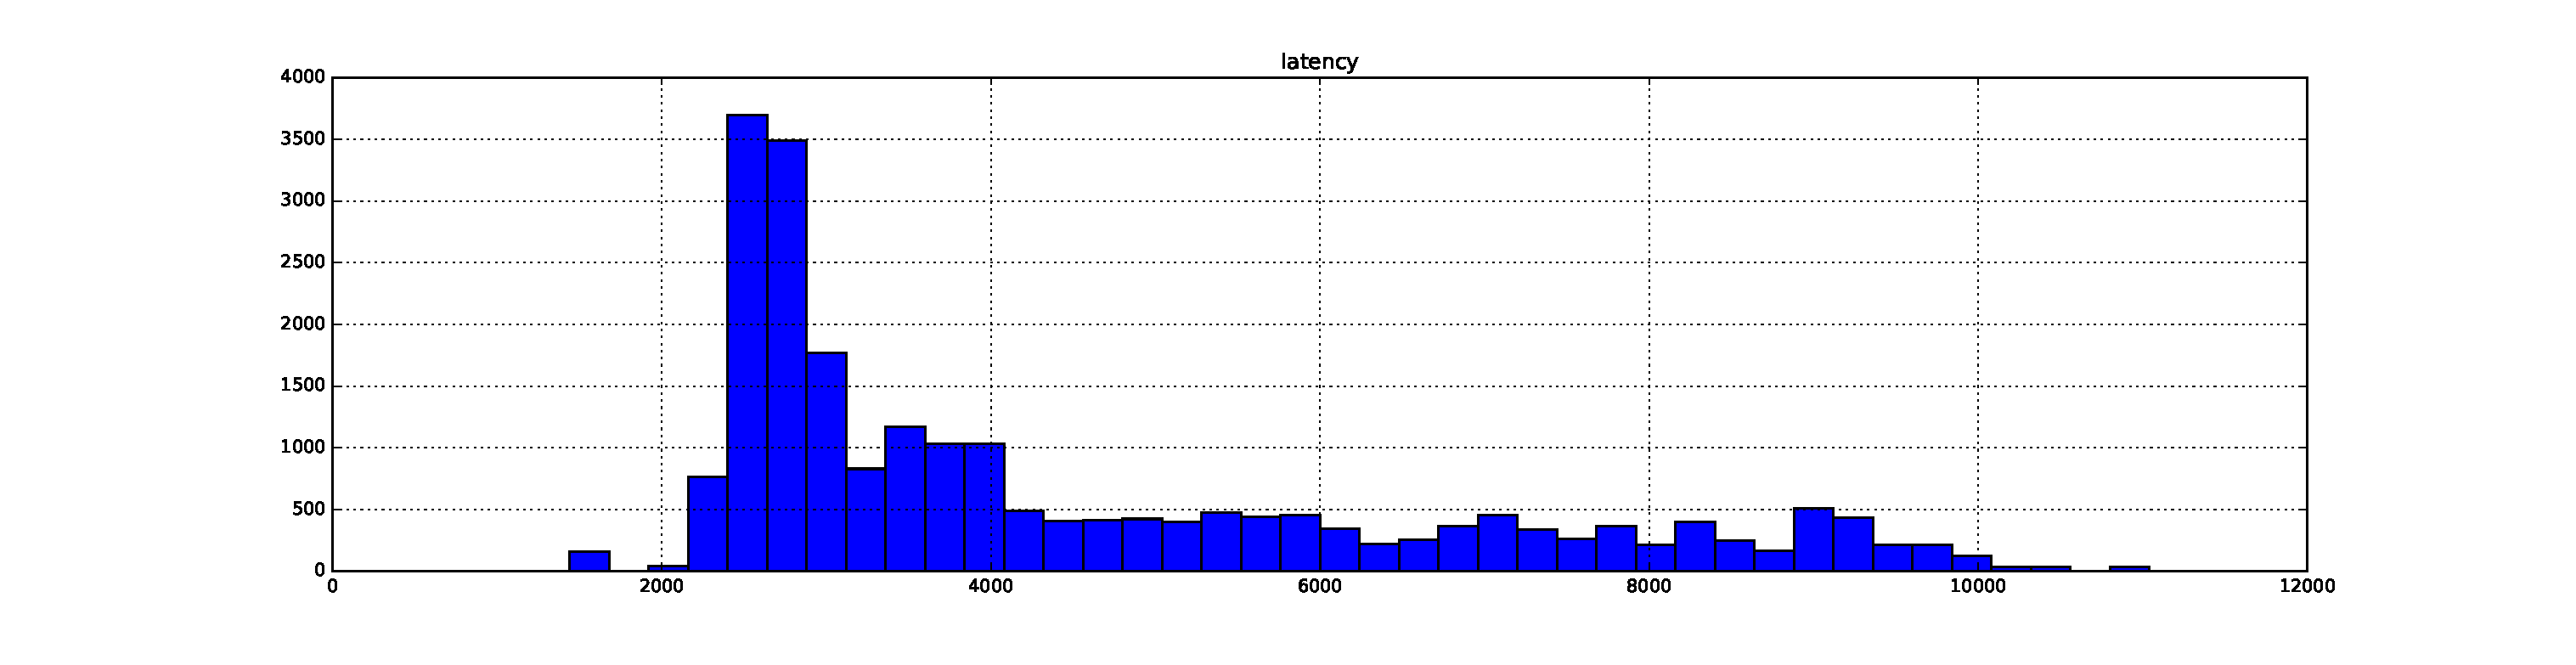
\includegraphics[width=\textwidth]{spark/4_4_1}
        \caption{4 Node latency histogram}
        \label{fig_partial_queue}
    \end{subfigure}
        \begin{subfigure}[b]{0.49\textwidth}
        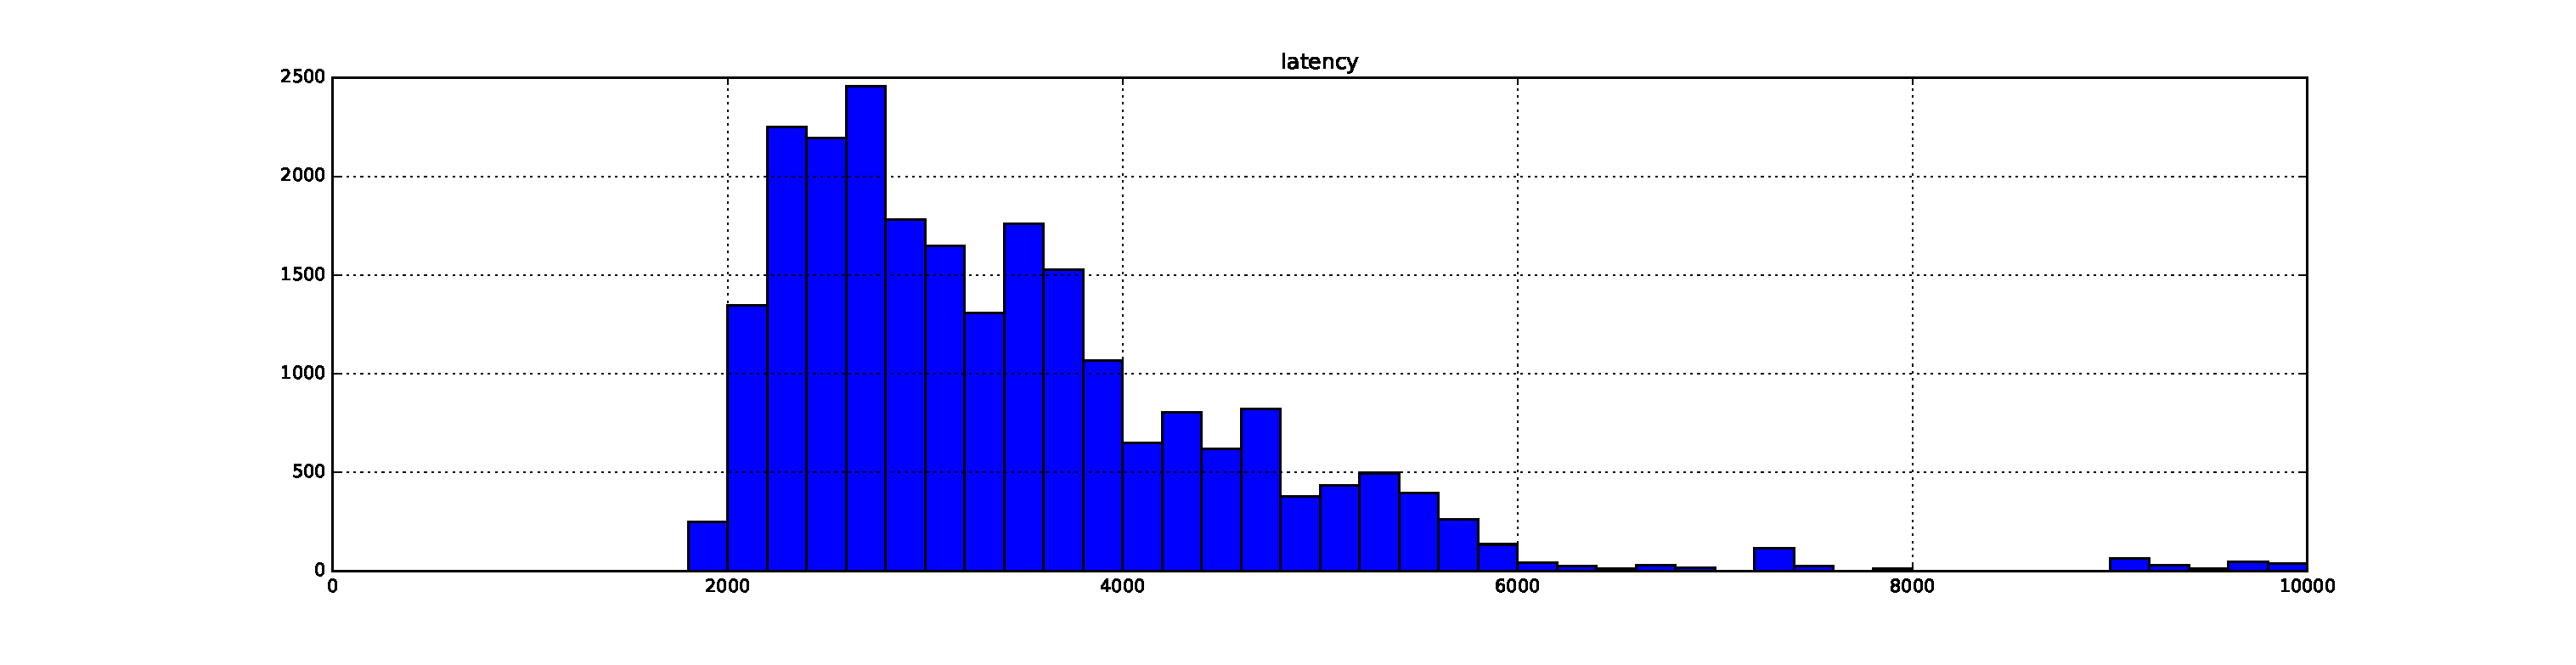
\includegraphics[width=\textwidth]{spark/8_4_1}
        \caption{8 Node latency histogram}
        \label{fig_partial_queue}
    \end{subfigure}


    \begin{subfigure}[b]{0.49\textwidth}
        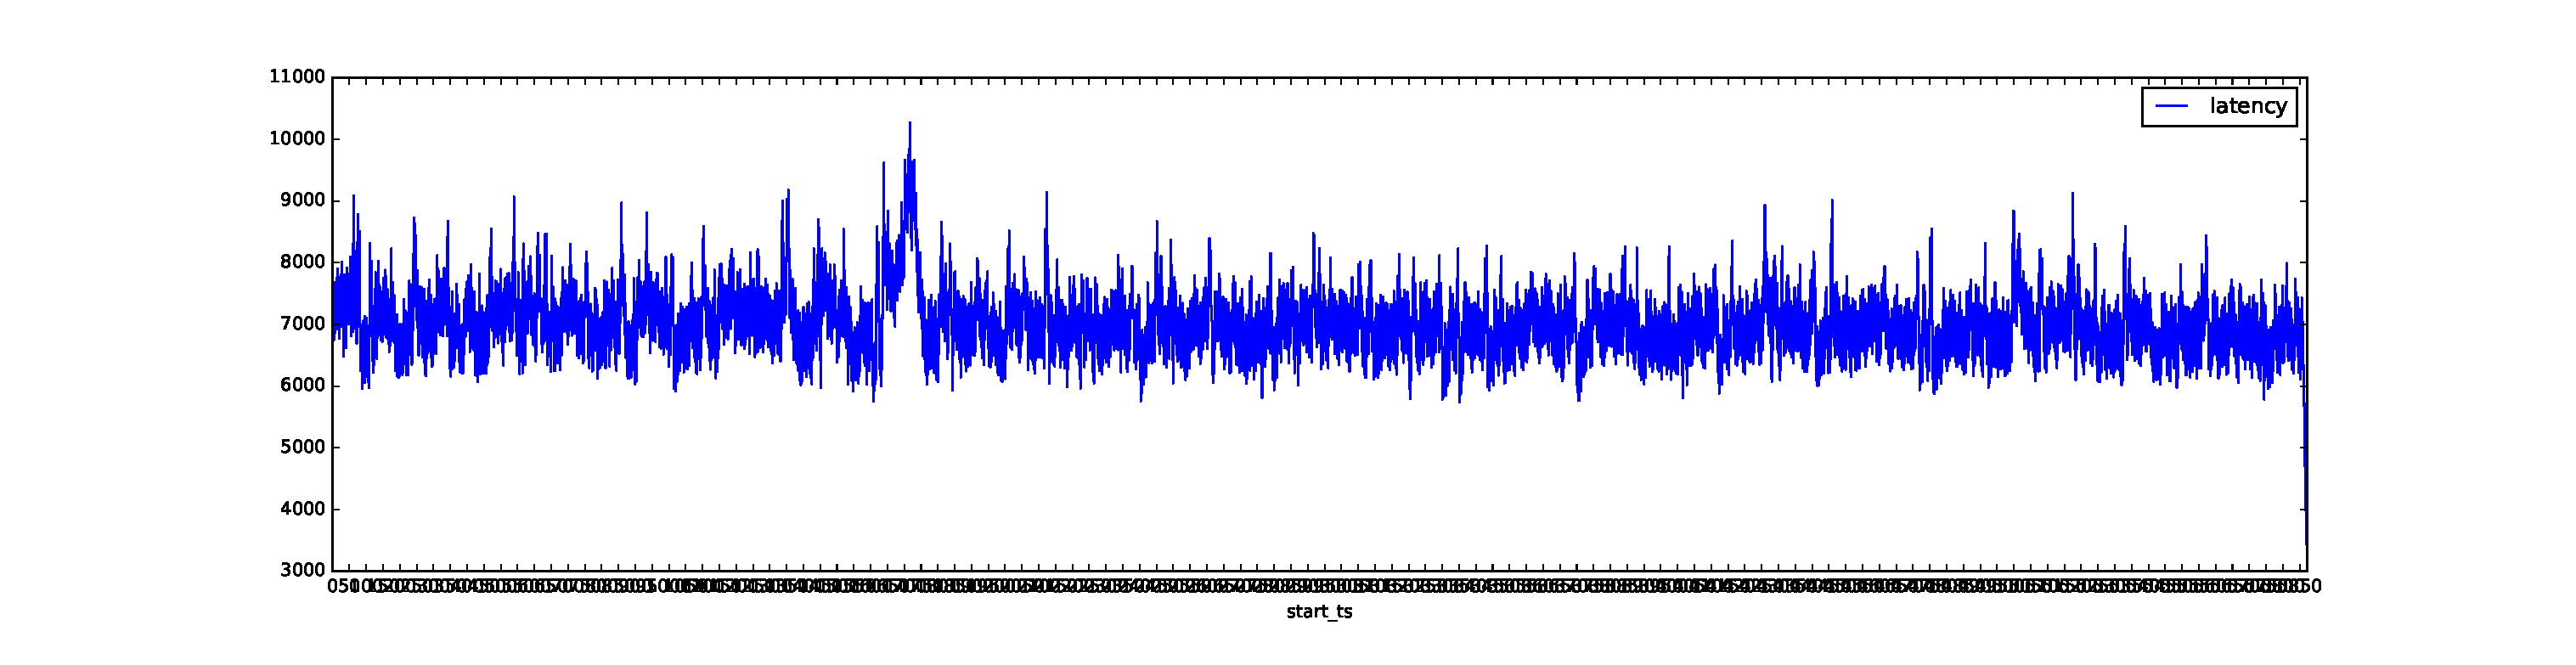
\includegraphics[width=\textwidth]{spark/2_4_2}
        \caption{2 Node latency time series}
        \label{fig_no_queue}
    \end{subfigure}
    ~ %add desired spacing between images, e. g. ~, \quad, \qquad, \hfill etc. 
      %(or a blank line to force the subfigure onto a new line)
    \begin{subfigure}[b]{0.49\textwidth}
        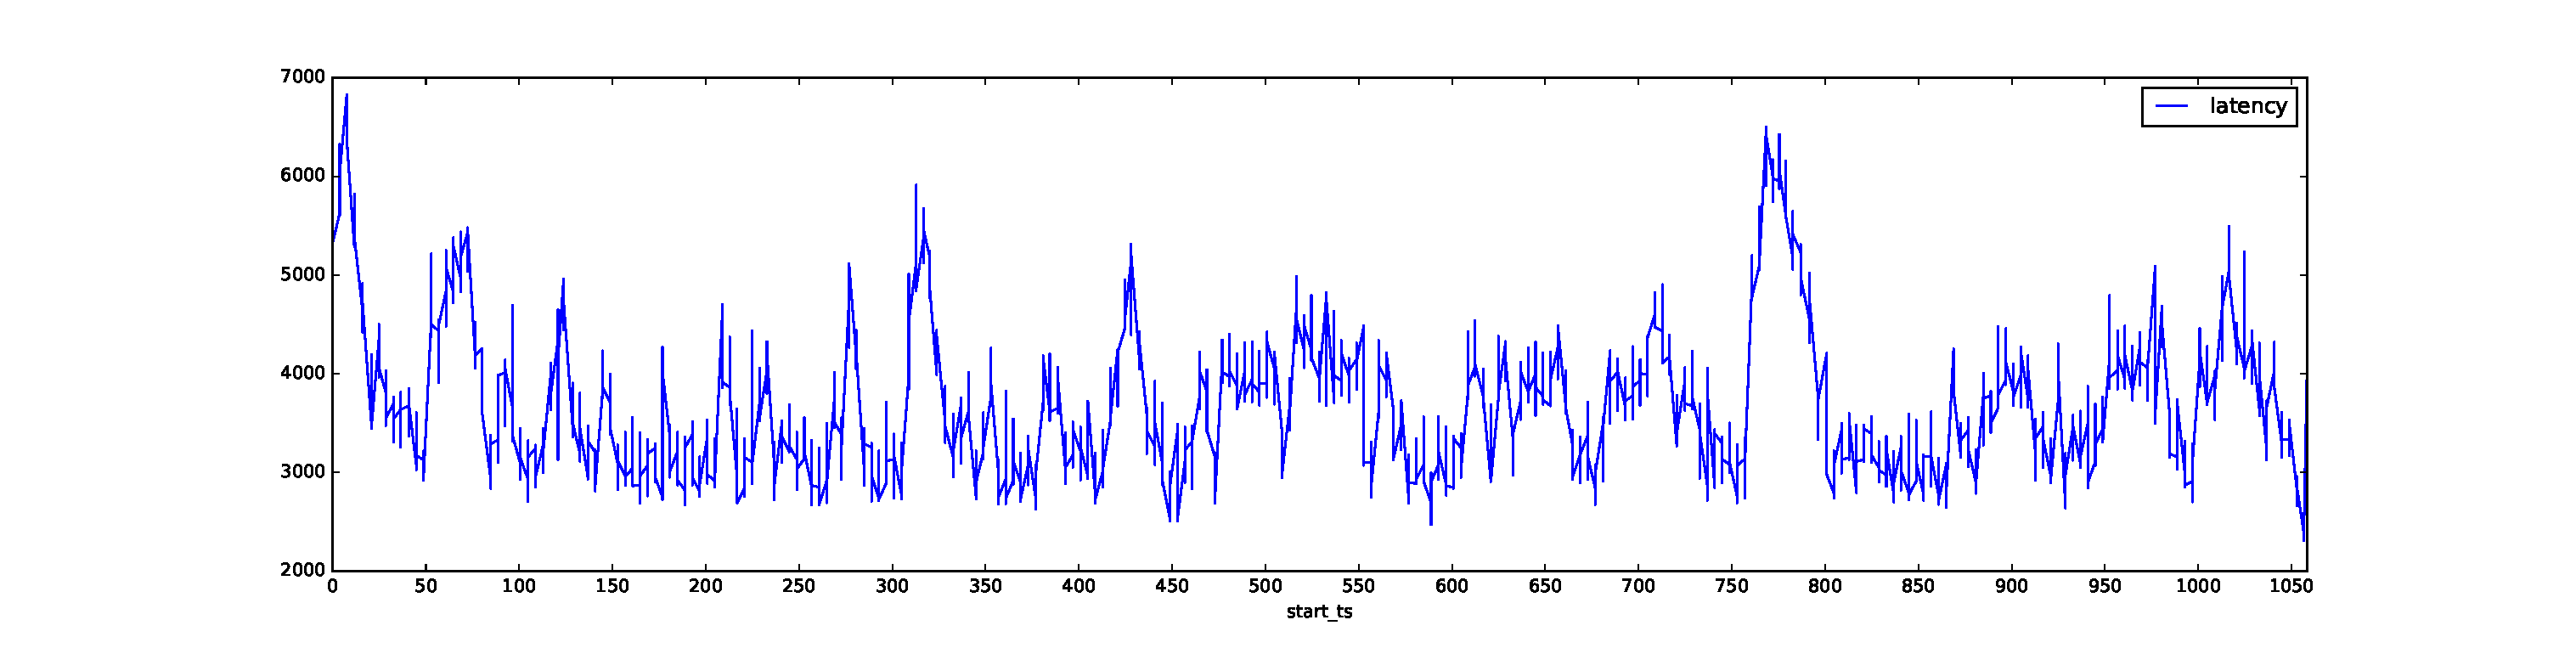
\includegraphics[width=\textwidth]{spark/3_4_2}
        \caption{3 Node latency time series}
        \label{fig_yes_queue}
    \end{subfigure}
    ~ %add desired spacing between images, e. g. ~, \quad, \qquad, \hfill etc. 
    %(or a blank line to force the subfigure onto a new line)
    \begin{subfigure}[b]{0.49\textwidth}
        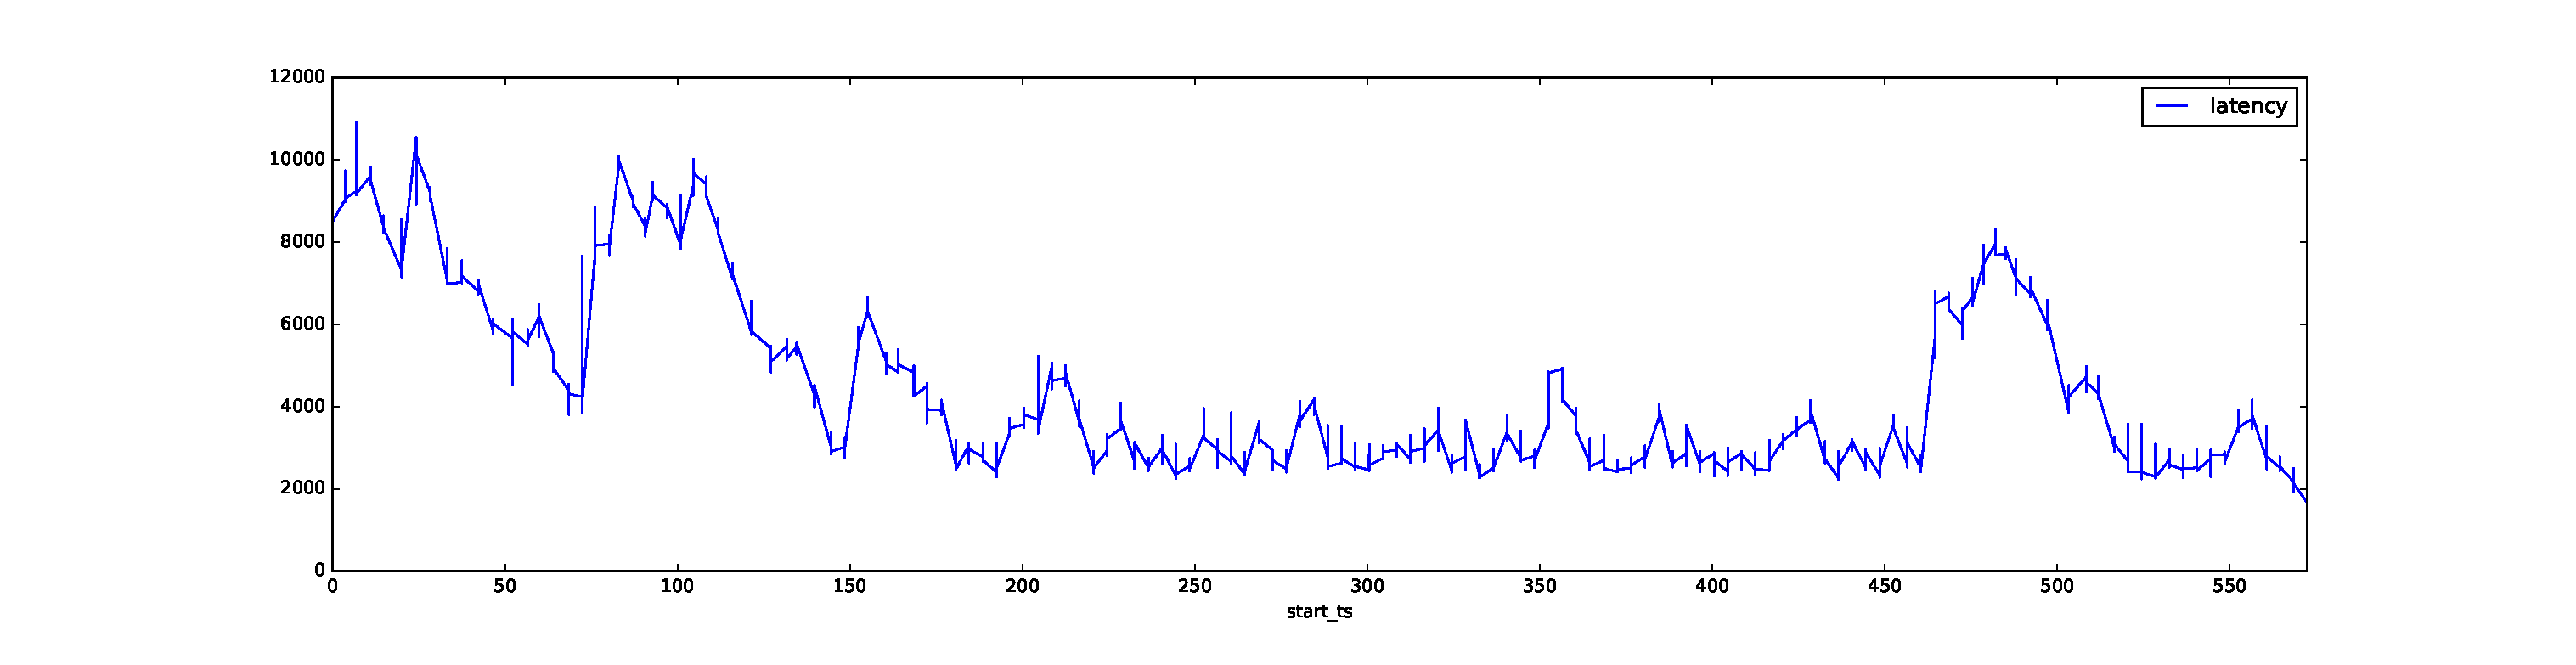
\includegraphics[width=\textwidth]{spark/4_4_2}
        \caption{4 Node latency time series}
        \label{fig_partial_queue}
    \end{subfigure}
        \begin{subfigure}[b]{0.49\textwidth}
        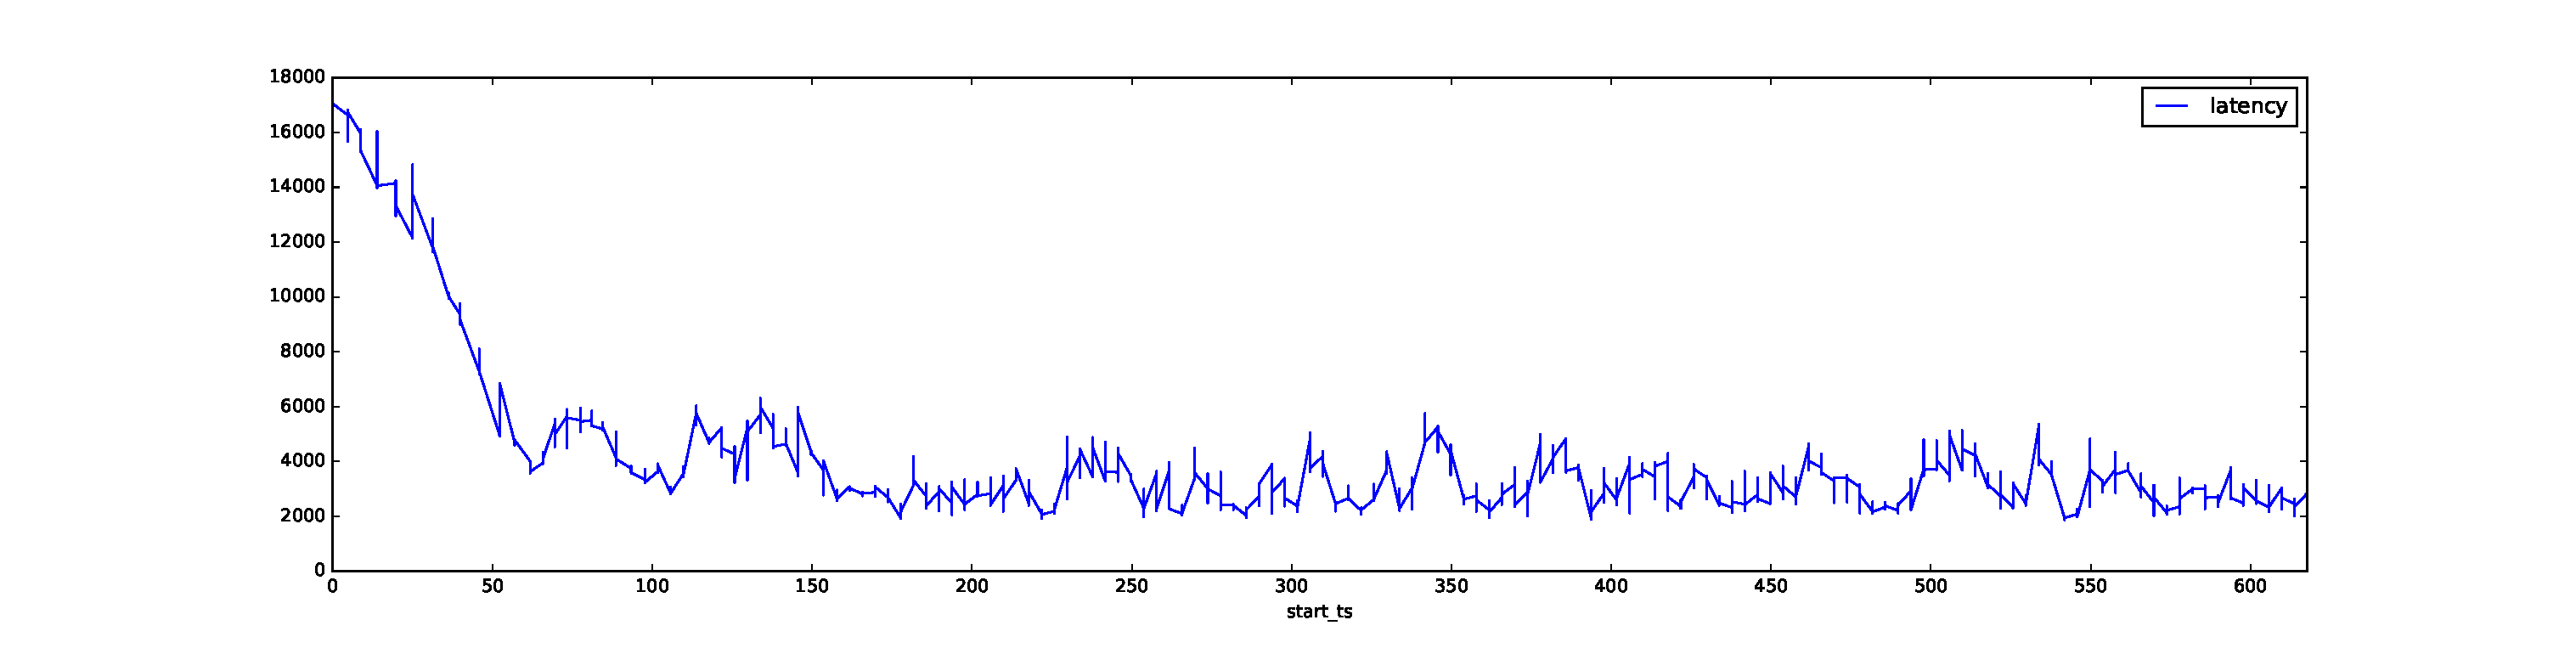
\includegraphics[width=\textwidth]{spark/8_4_2}
        \caption{8 Node latency time series}
        \label{fig_partial_queue}
    \end{subfigure}

    \label{fig_flink_agg_1}
        \caption{Latency of windowed aggregations for Spark (4 sec batch).}
\end{figure*}





\begin{figure*}
    \centering
    \begin{subfigure}[b]{0.49\textwidth}
        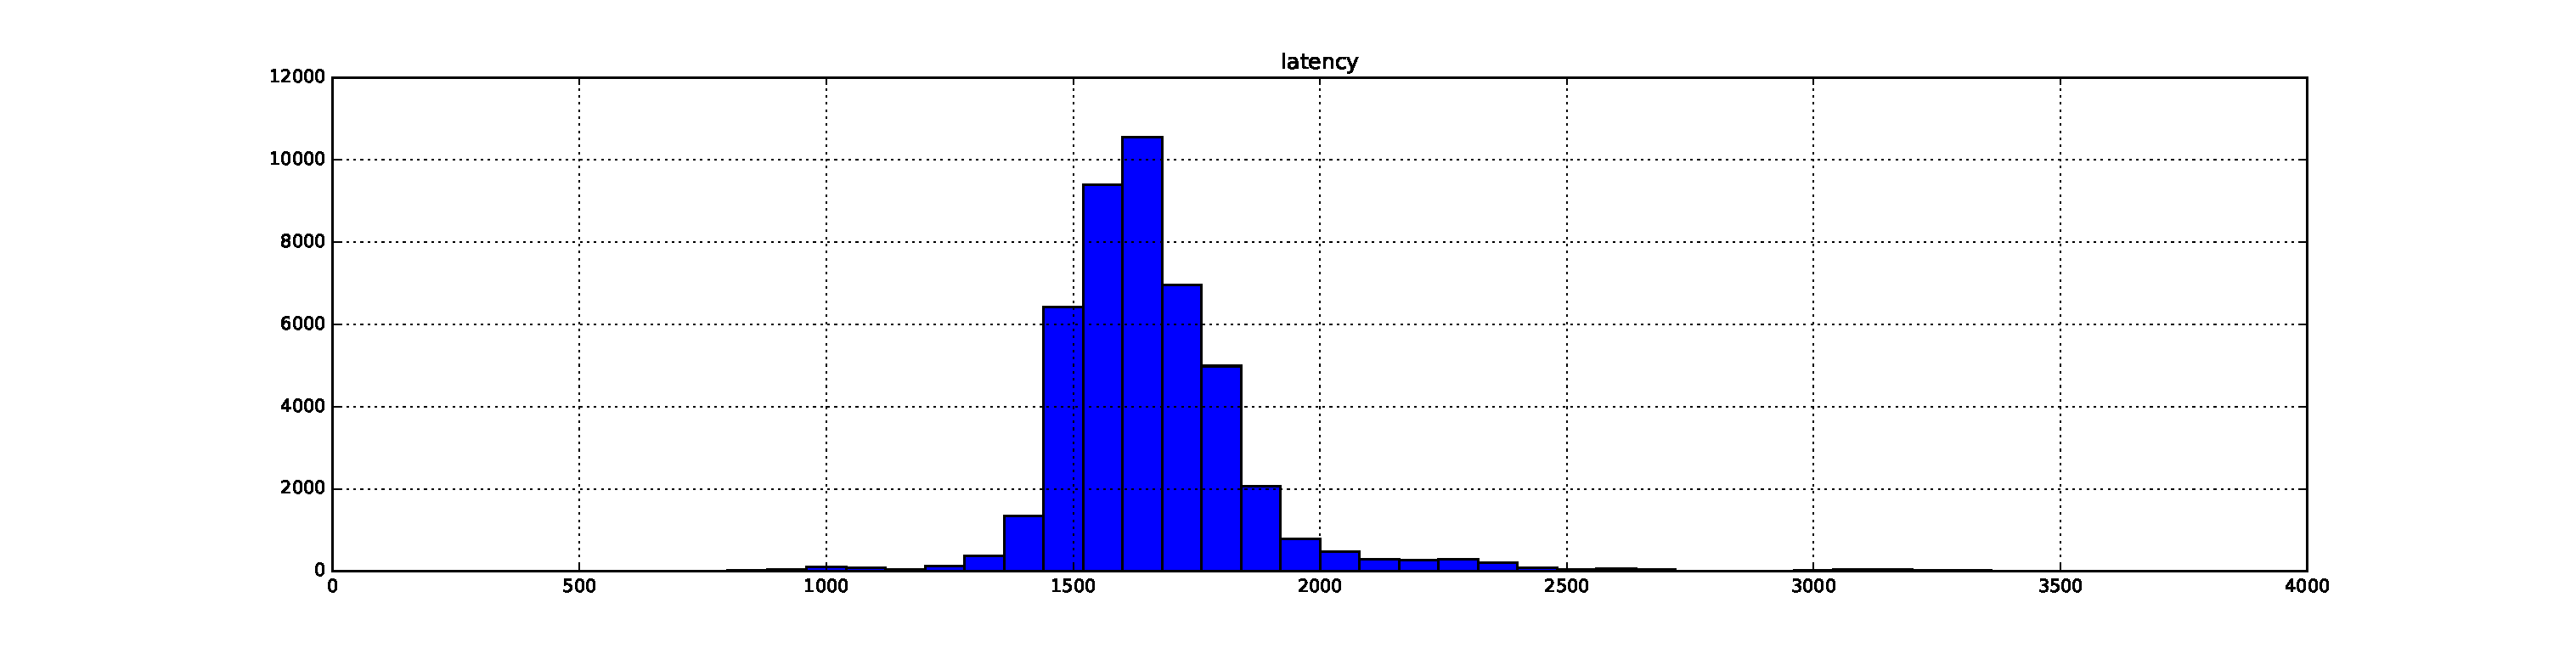
\includegraphics[width=\textwidth]{spark/2_2_1}
        \caption{2 Node latency histogram}
        \label{fig_no_queue}
    \end{subfigure}
    ~ %add desired spacing between images, e. g. ~, \quad, \qquad, \hfill etc. 
      %(or a blank line to force the subfigure onto a new line)
    \begin{subfigure}[b]{0.49\textwidth}
        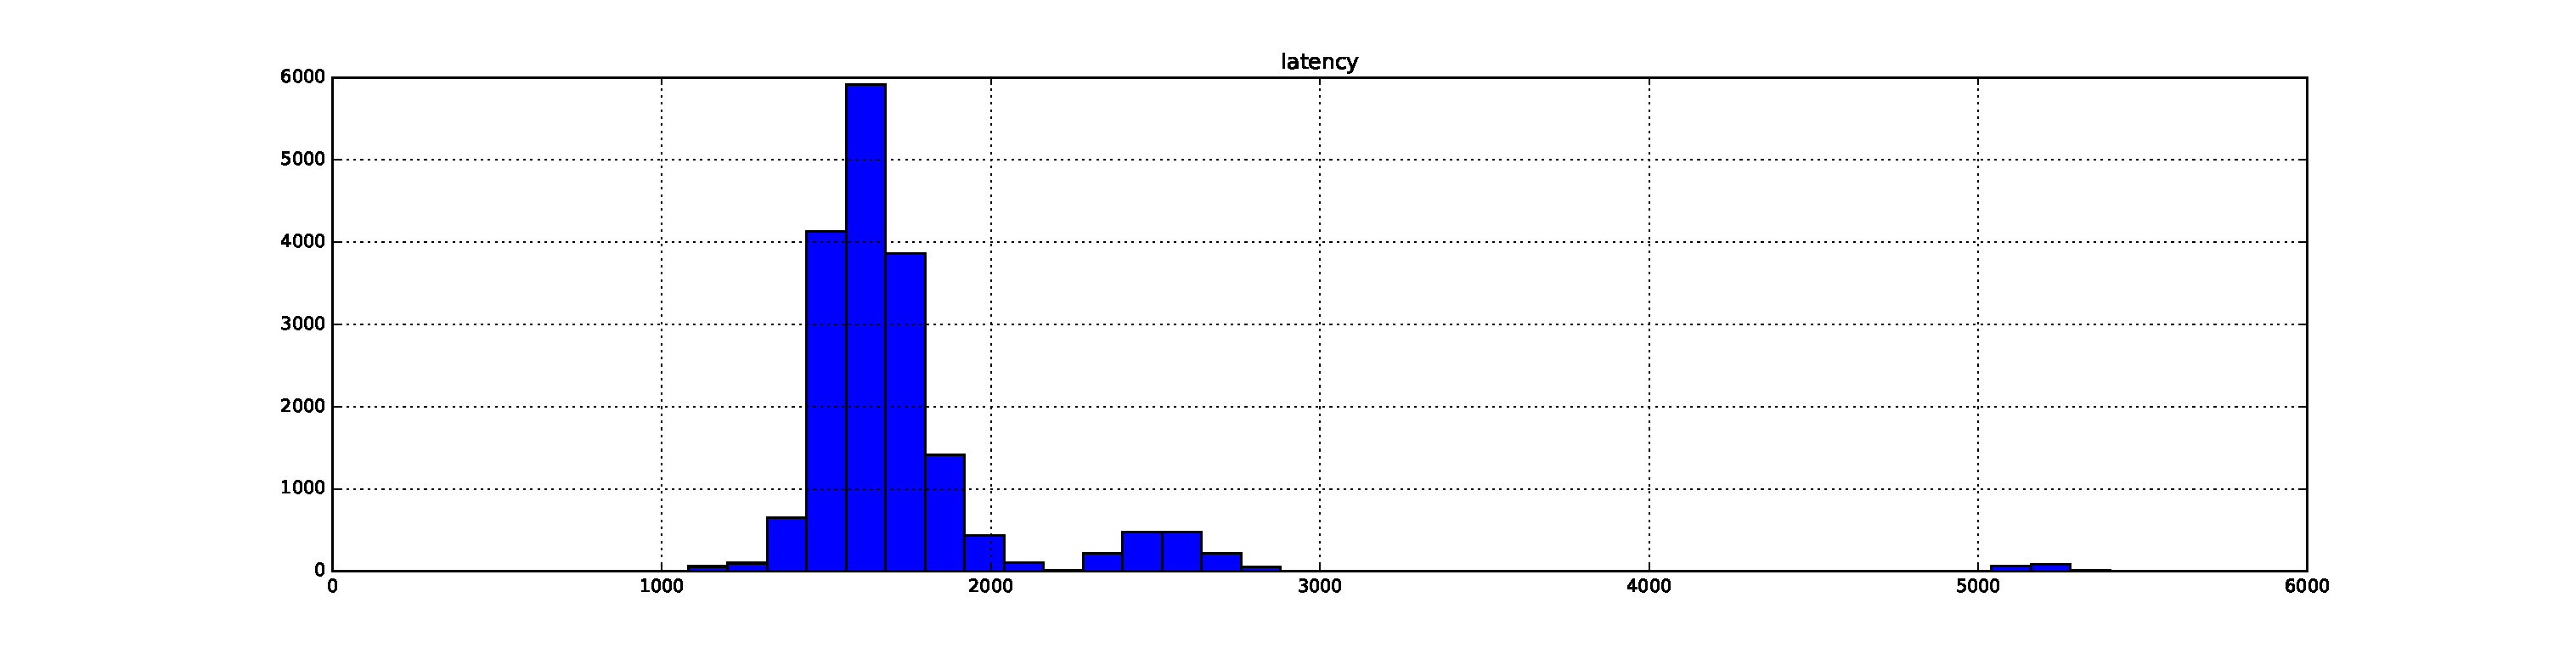
\includegraphics[width=\textwidth]{spark/3_2_1}
        \caption{3 Node latency histogram}
        \label{fig_yes_queue}
    \end{subfigure}
    ~ %add desired spacing between images, e. g. ~, \quad, \qquad, \hfill etc. 
    %(or a blank line to force the subfigure onto a new line)
    \begin{subfigure}[b]{0.49\textwidth}
        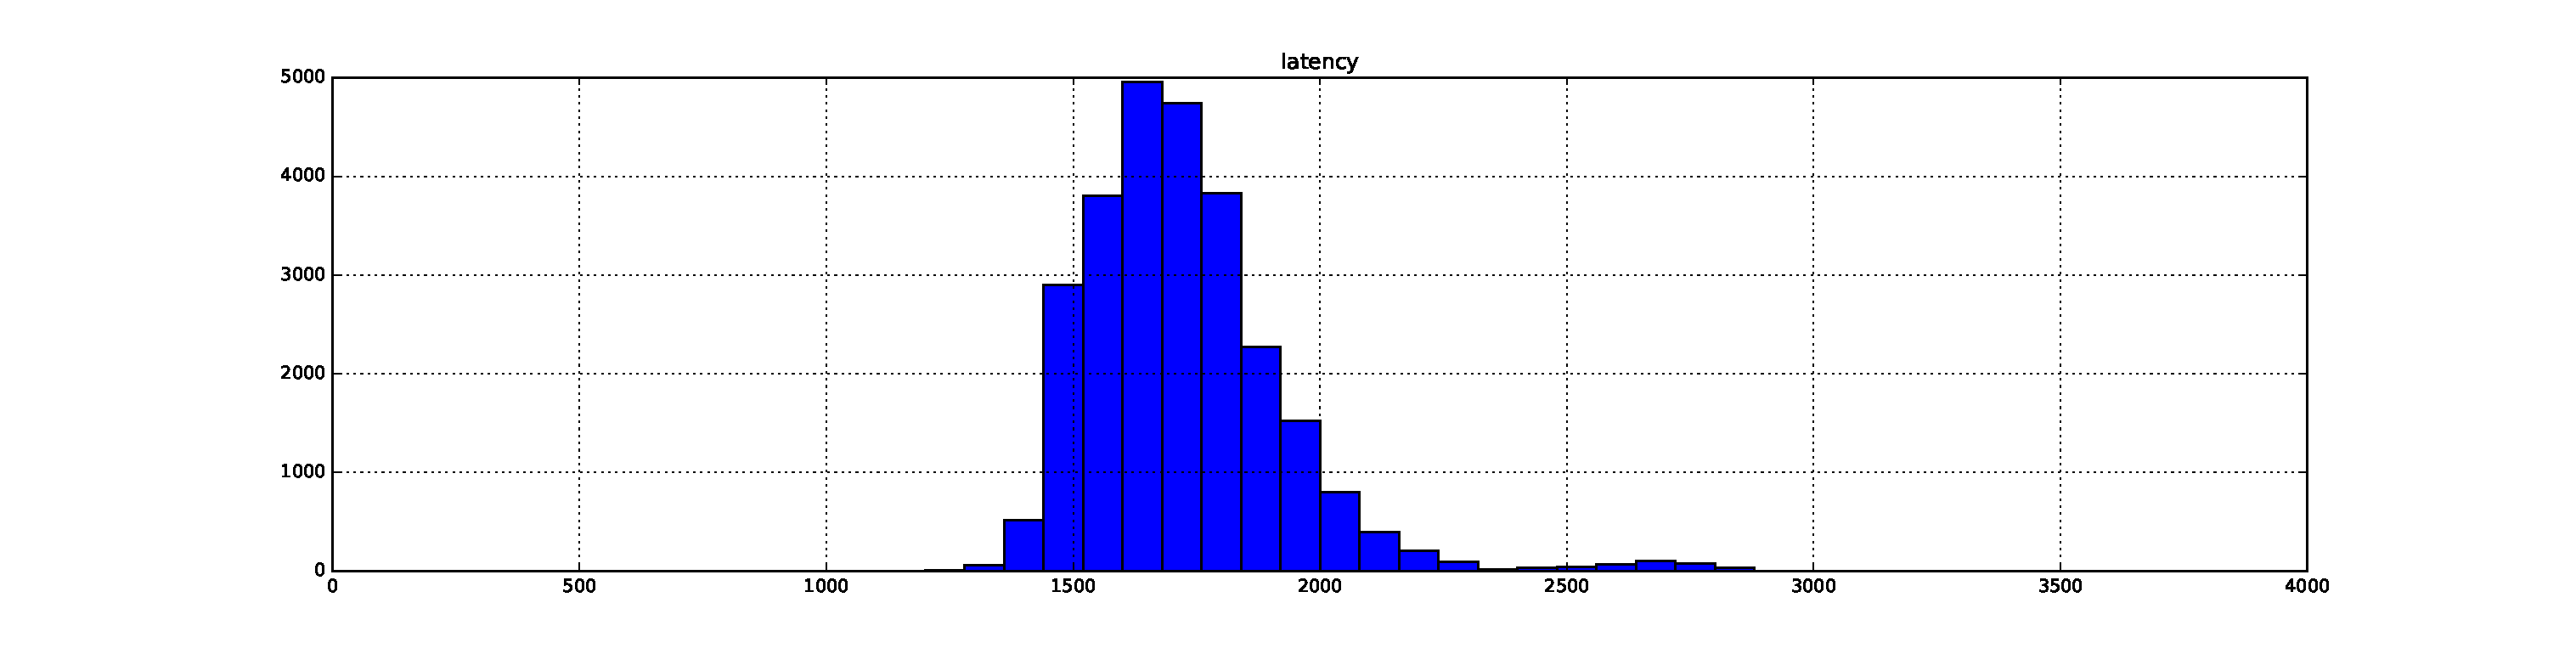
\includegraphics[width=\textwidth]{spark/4_2_1}
        \caption{4 Node latency histogram}
        \label{fig_partial_queue}
    \end{subfigure}
        \begin{subfigure}[b]{0.49\textwidth}
        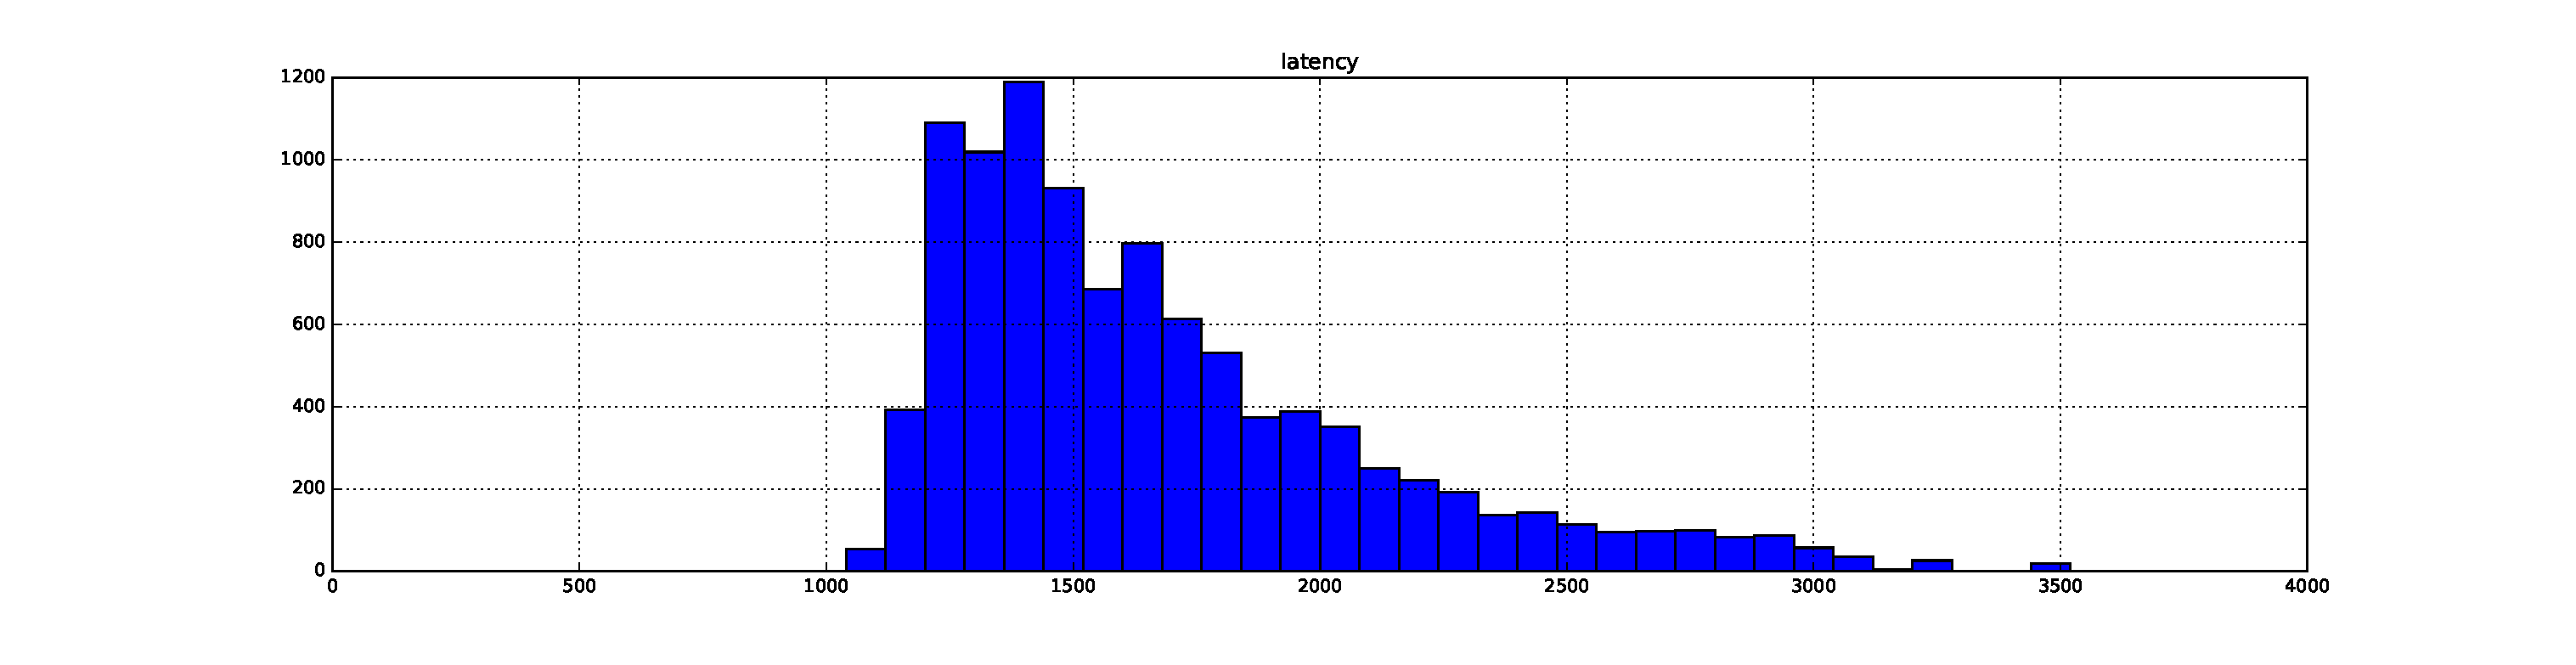
\includegraphics[width=\textwidth]{spark/8_2_1}
        \caption{8 Node latency histogram}
        \label{fig_partial_queue}
    \end{subfigure}


    \begin{subfigure}[b]{0.49\textwidth}
        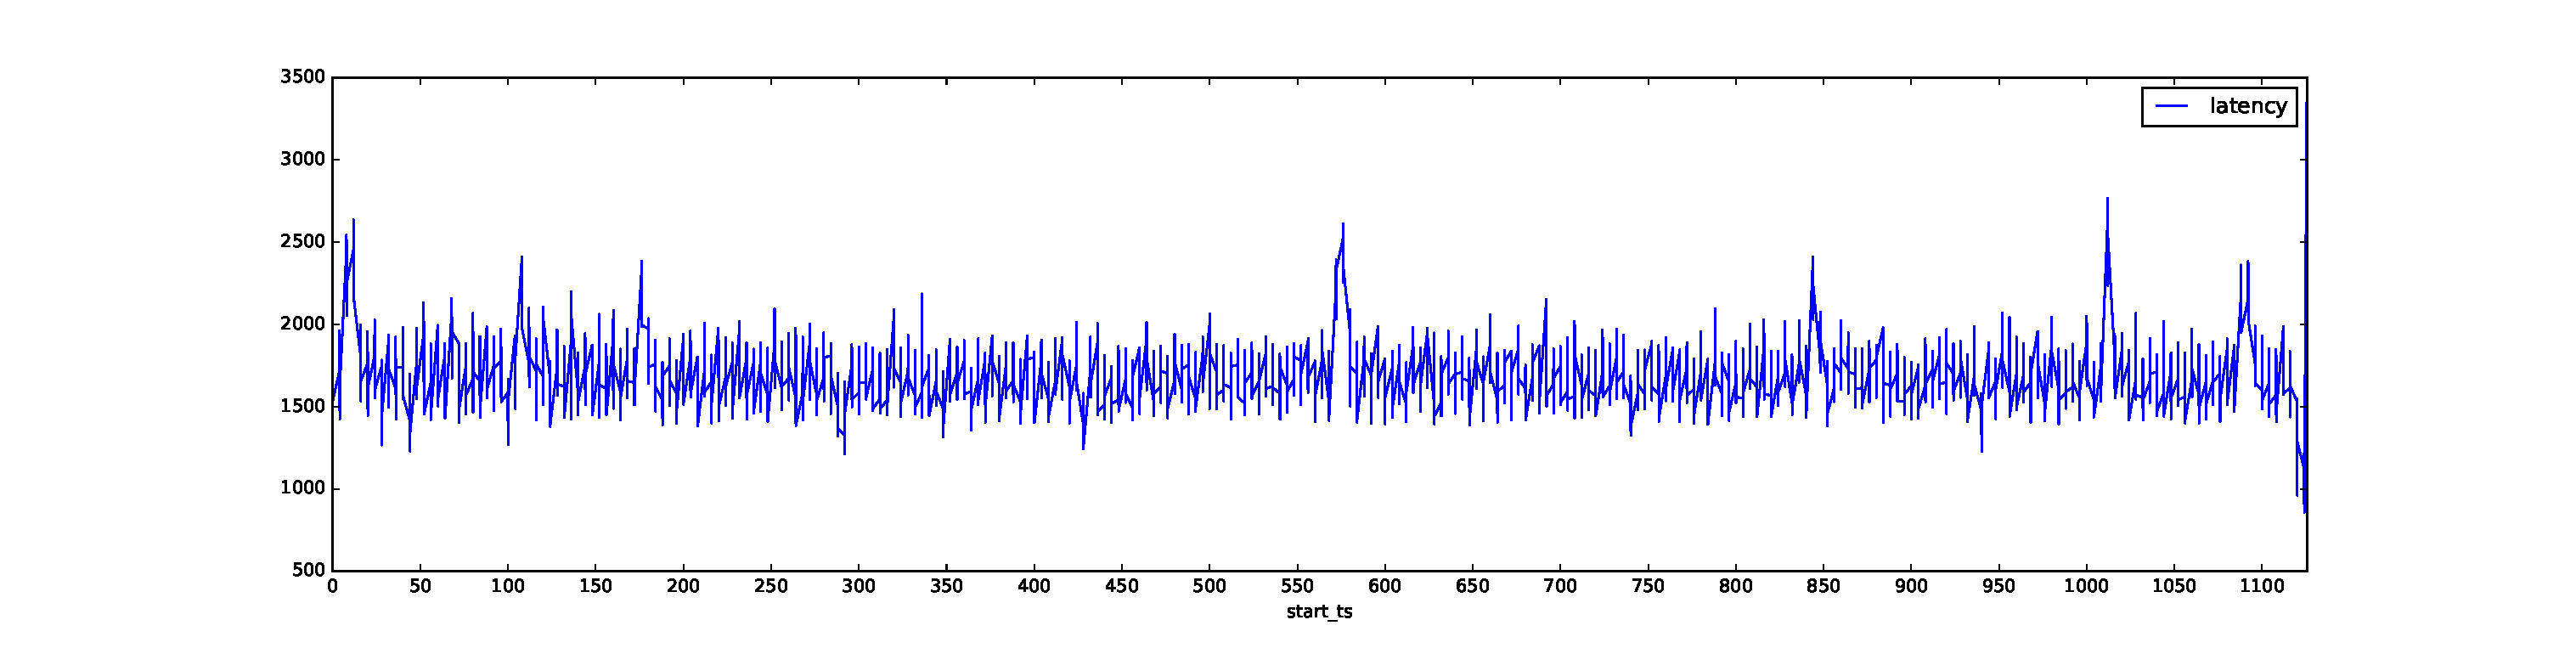
\includegraphics[width=\textwidth]{spark/2_2_2}
        \caption{2 Node latency time series}
        \label{fig_no_queue}
    \end{subfigure}
    ~ %add desired spacing between images, e. g. ~, \quad, \qquad, \hfill etc. 
      %(or a blank line to force the subfigure onto a new line)
    \begin{subfigure}[b]{0.49\textwidth}
        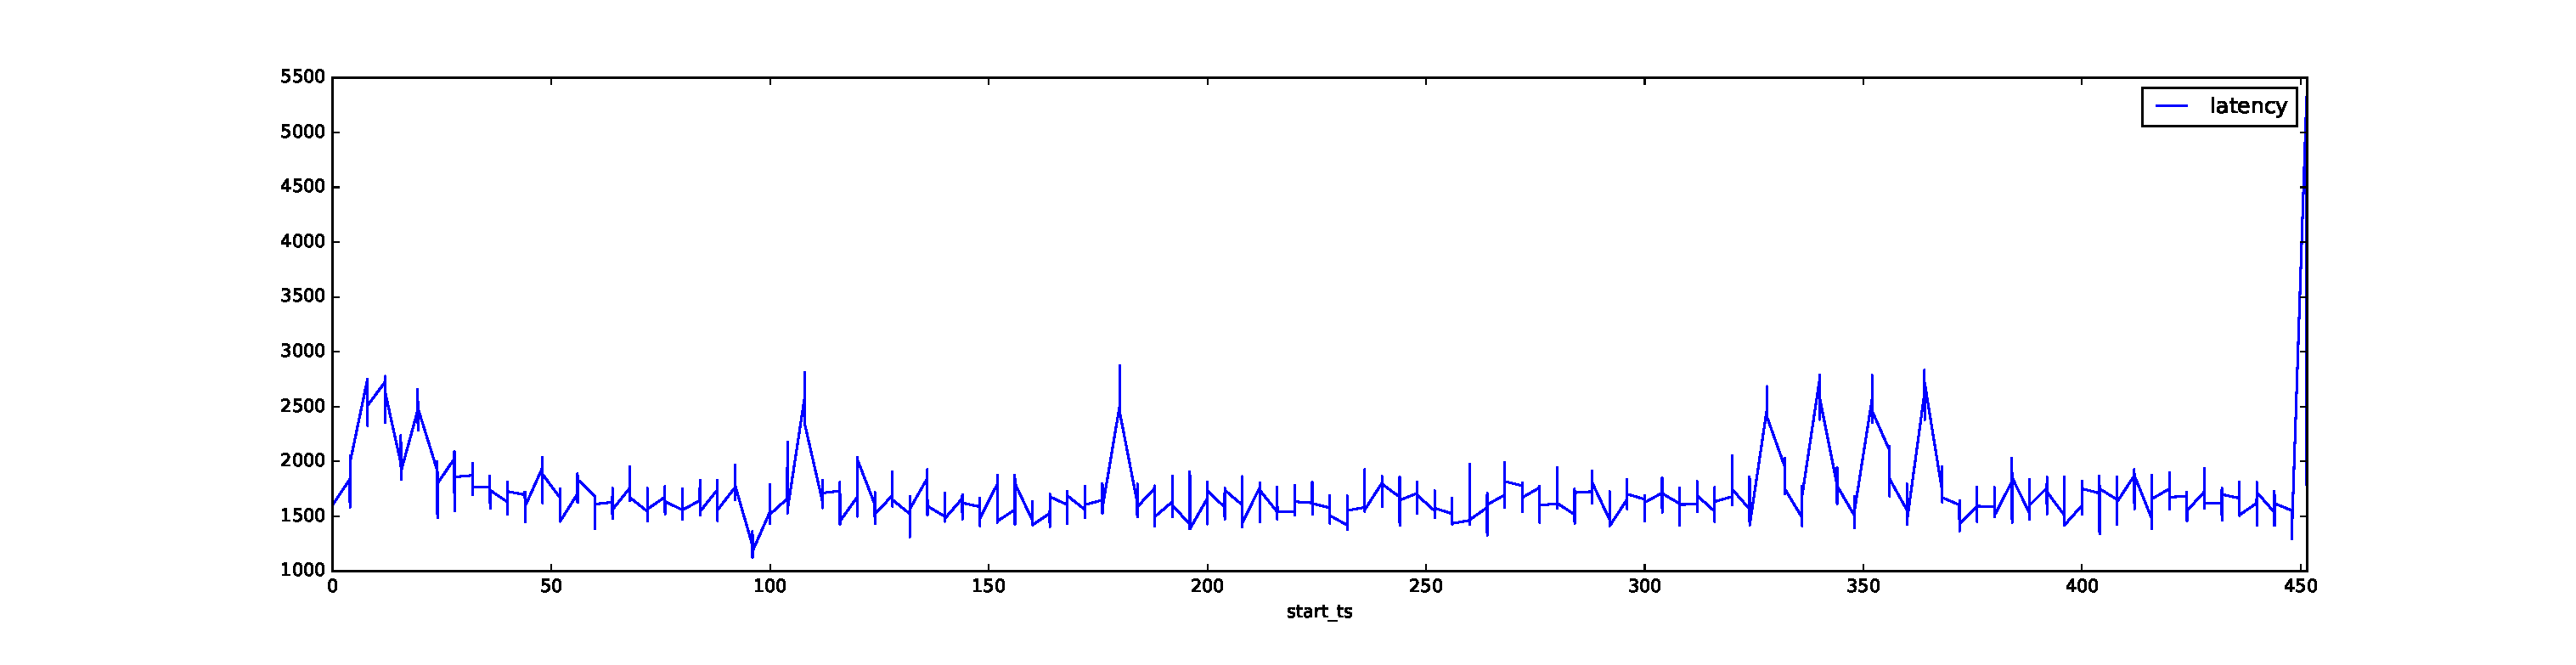
\includegraphics[width=\textwidth]{spark/3_2_2}
        \caption{3 Node latency time series}
        \label{fig_yes_queue}
    \end{subfigure}
    ~ %add desired spacing between images, e. g. ~, \quad, \qquad, \hfill etc. 
    %(or a blank line to force the subfigure onto a new line)
    \begin{subfigure}[b]{0.49\textwidth}
        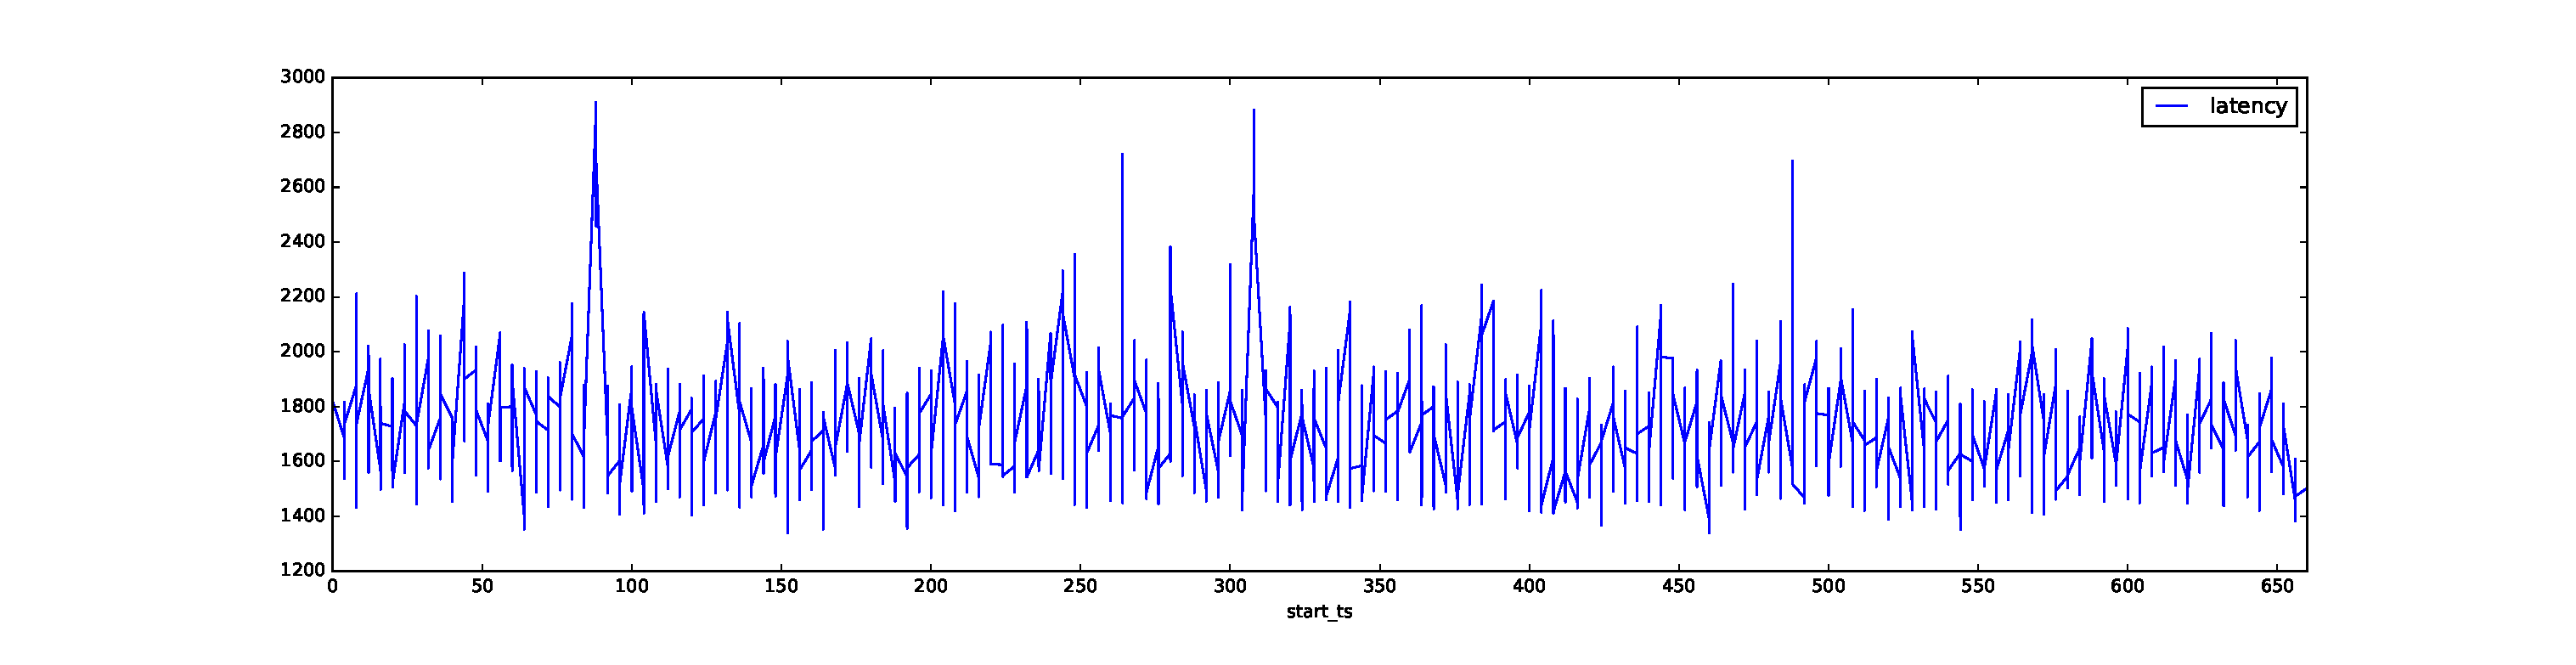
\includegraphics[width=\textwidth]{spark/4_2_2}
        \caption{4 Node latency time series}
        \label{fig_partial_queue}
    \end{subfigure}
        \begin{subfigure}[b]{0.49\textwidth}
        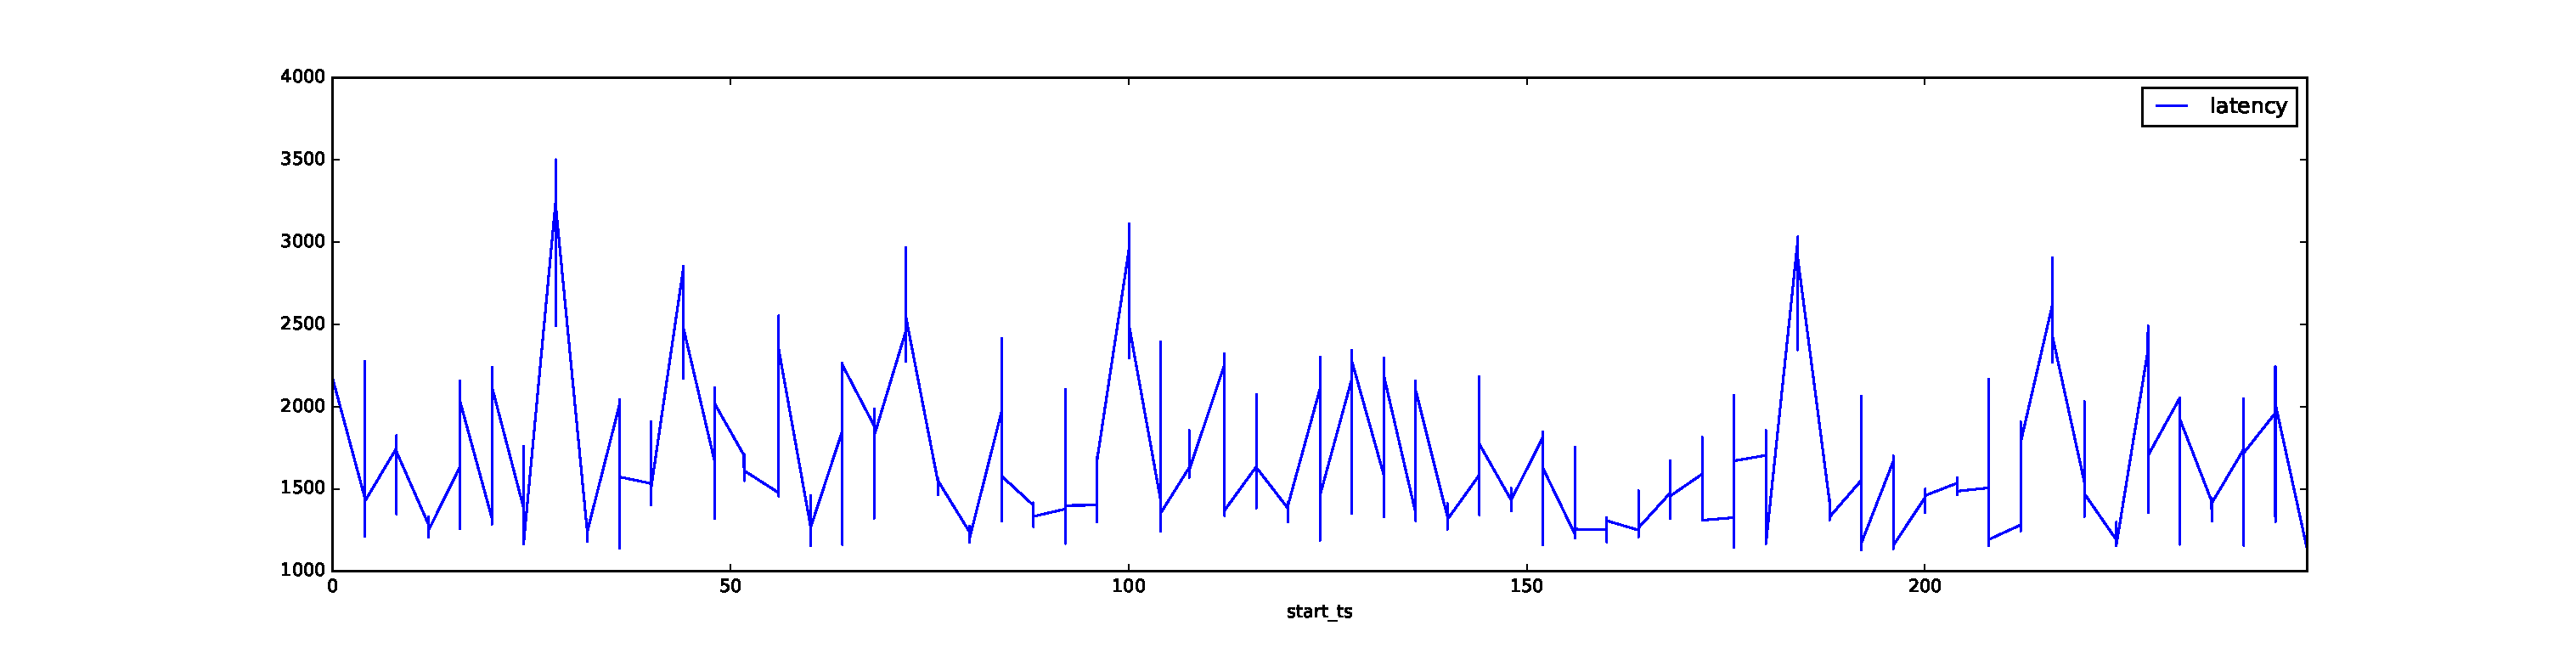
\includegraphics[width=\textwidth]{spark/8_2_2}
        \caption{8 Node latency time series}
        \label{fig_partial_queue}
    \end{subfigure}

    \label{fig_flink_agg_1}
        \caption{Latency of windowed aggregations for Spark (2 sec batch).}
\end{figure*}





\subsubsection{Flink}





\begin{figure*}
    \centering
    \begin{subfigure}[b]{0.49\textwidth}
        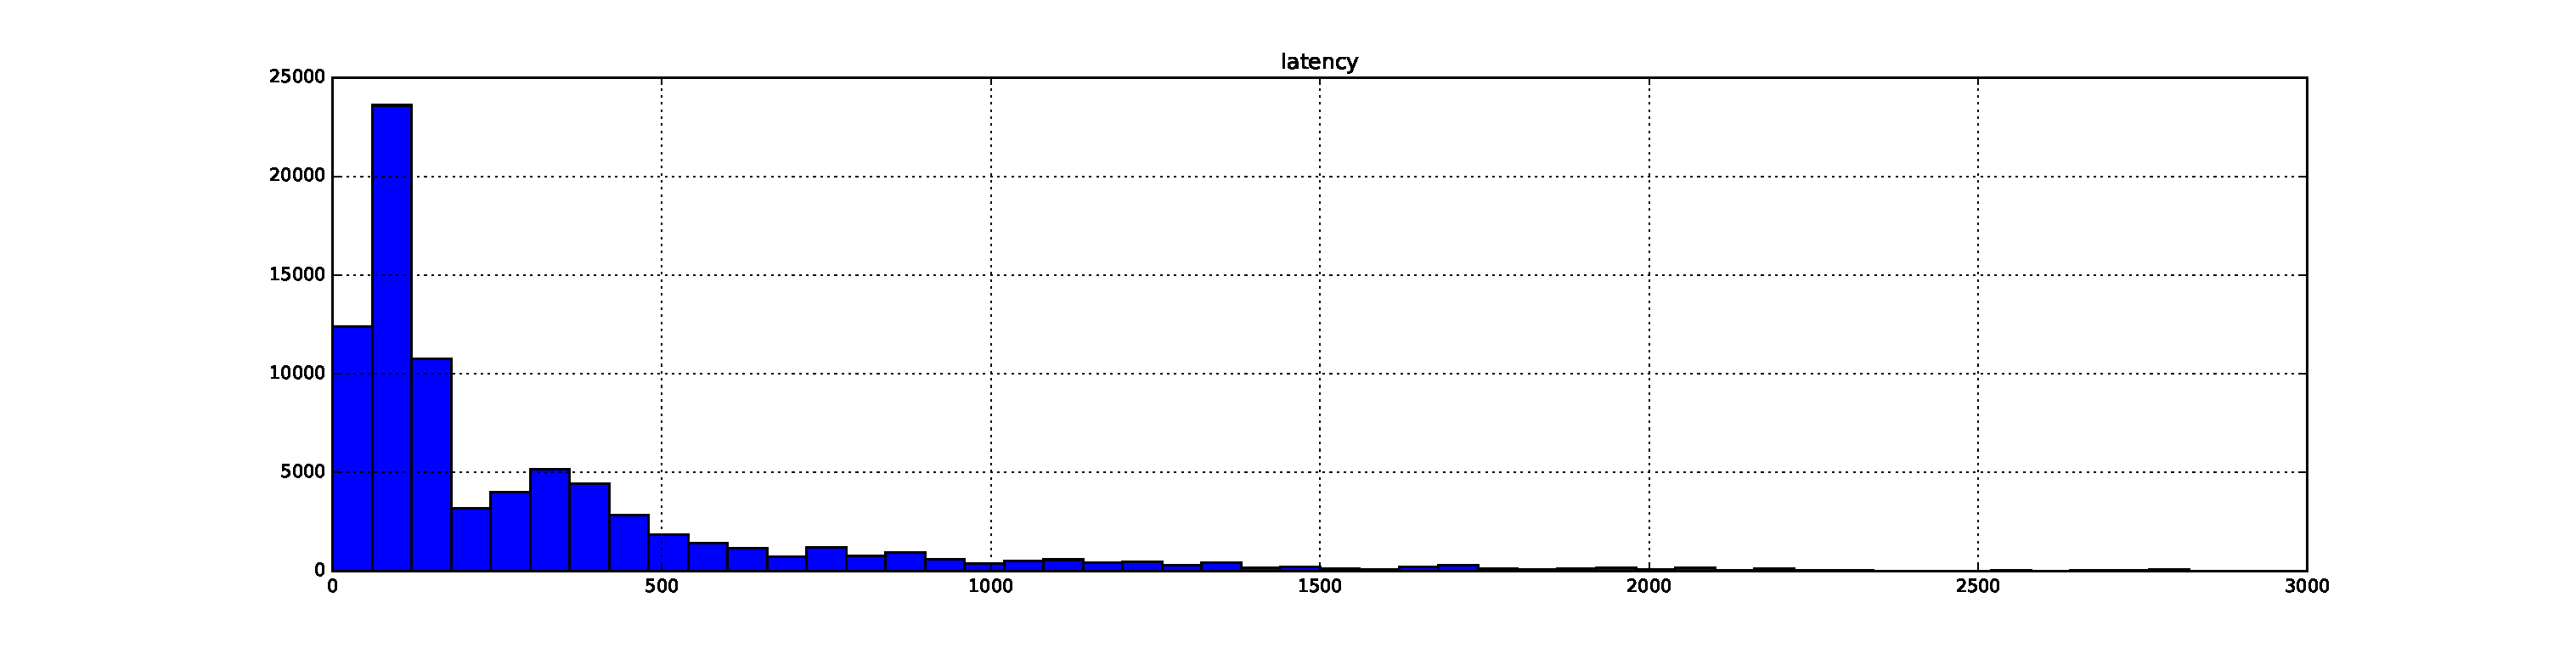
\includegraphics[width=\textwidth]{flink/2_1}
        \caption{2 Node latency histogram}
        \label{fig_no_queue}
    \end{subfigure}
    ~ %add desired spacing between images, e. g. ~, \quad, \qquad, \hfill etc. 
      %(or a blank line to force the subfigure onto a new line)
    \begin{subfigure}[b]{0.49\textwidth}
        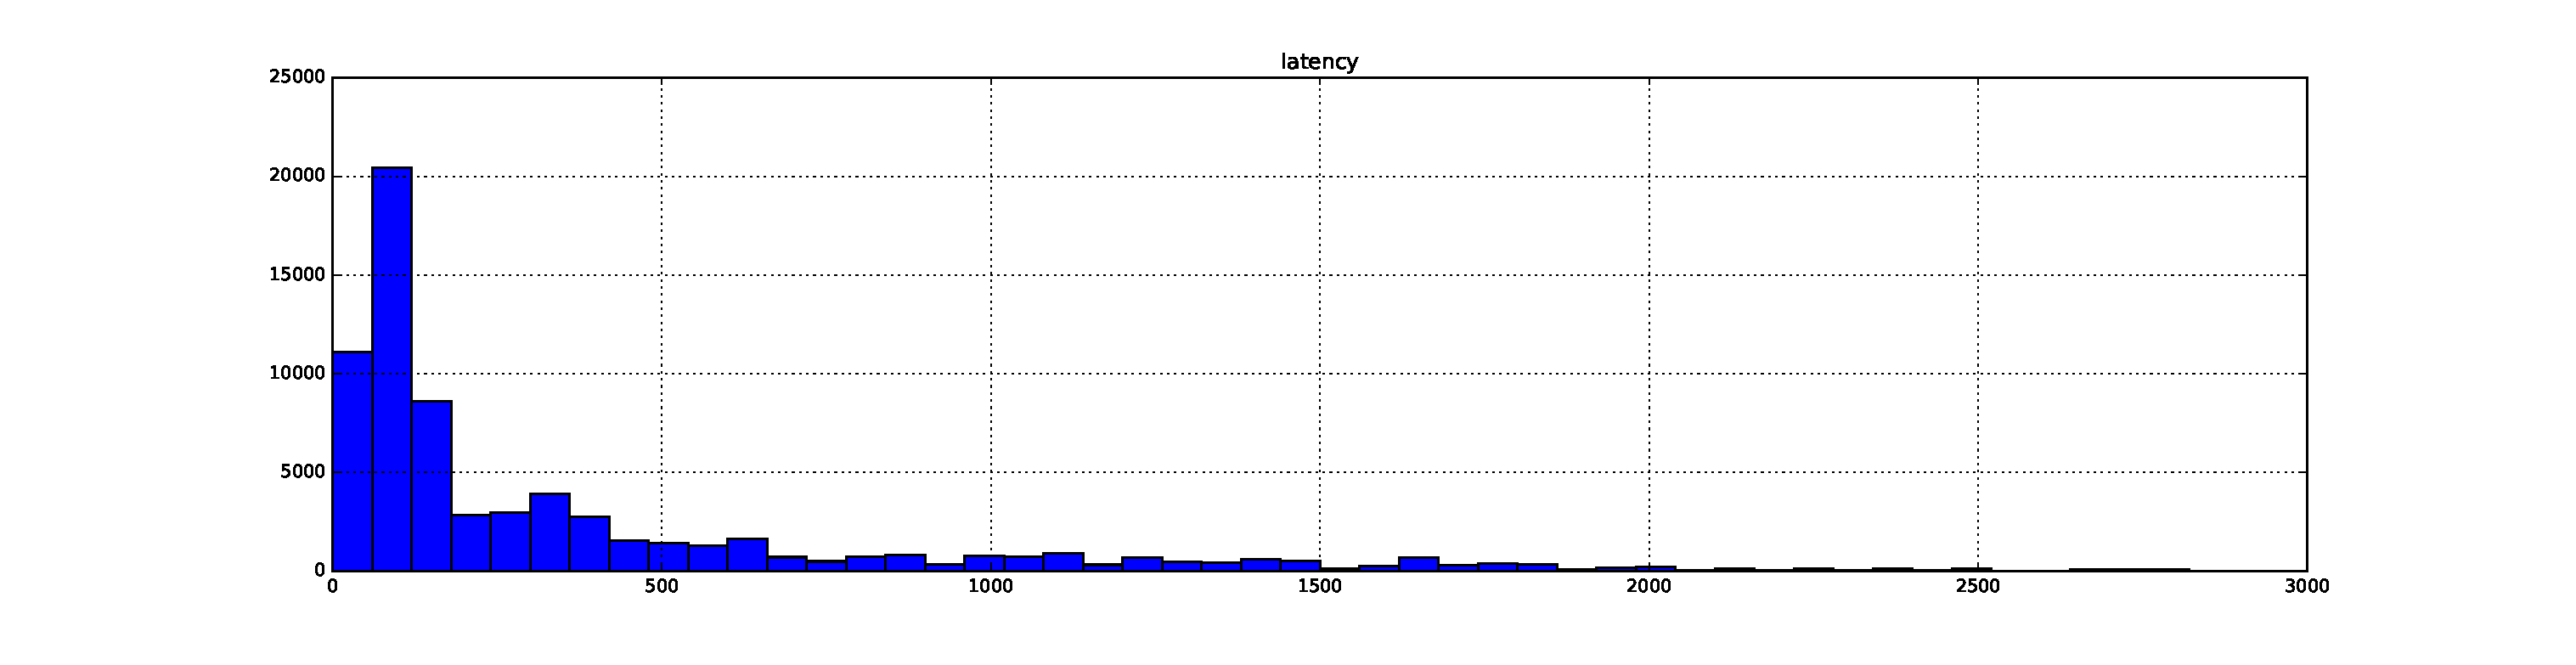
\includegraphics[width=\textwidth]{flink/3_1}
        \caption{3 Node latency histogram}
        \label{fig_yes_queue}
    \end{subfigure}
    ~ %add desired spacing between images, e. g. ~, \quad, \qquad, \hfill etc. 
    %(or a blank line to force the subfigure onto a new line)
    \begin{subfigure}[b]{0.49\textwidth}
        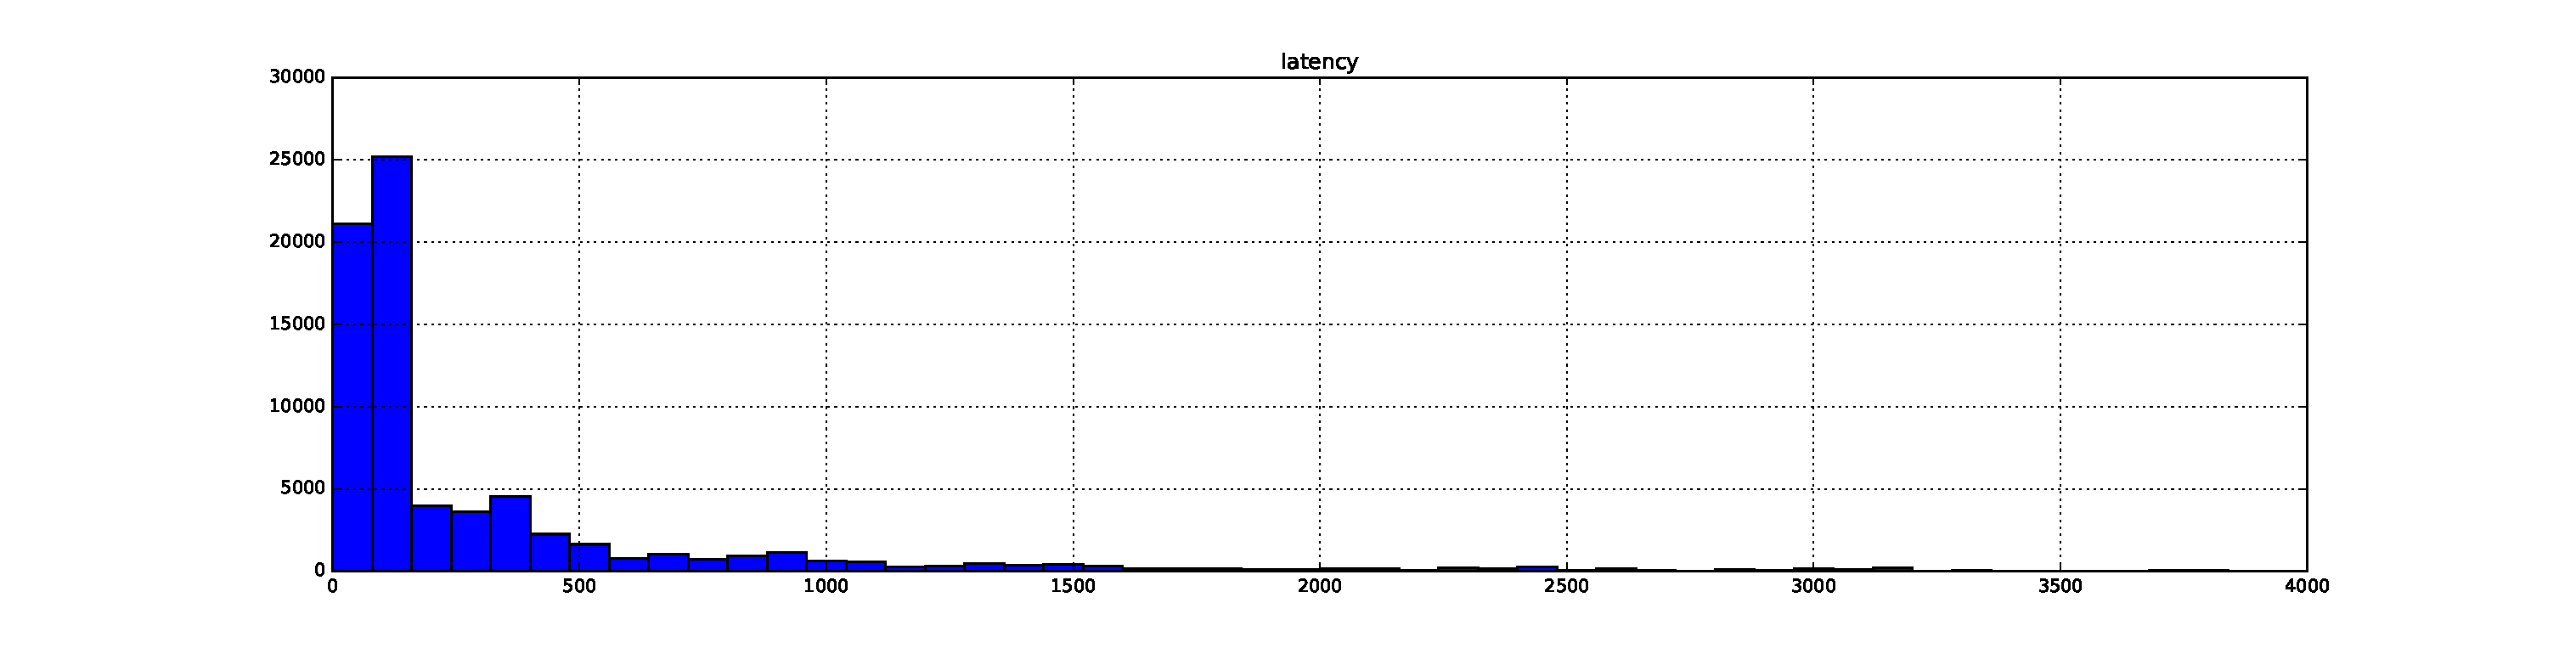
\includegraphics[width=\textwidth]{flink/4_1}
        \caption{4 Node latency histogram}
        \label{fig_partial_queue}
    \end{subfigure}
        \begin{subfigure}[b]{0.49\textwidth}
        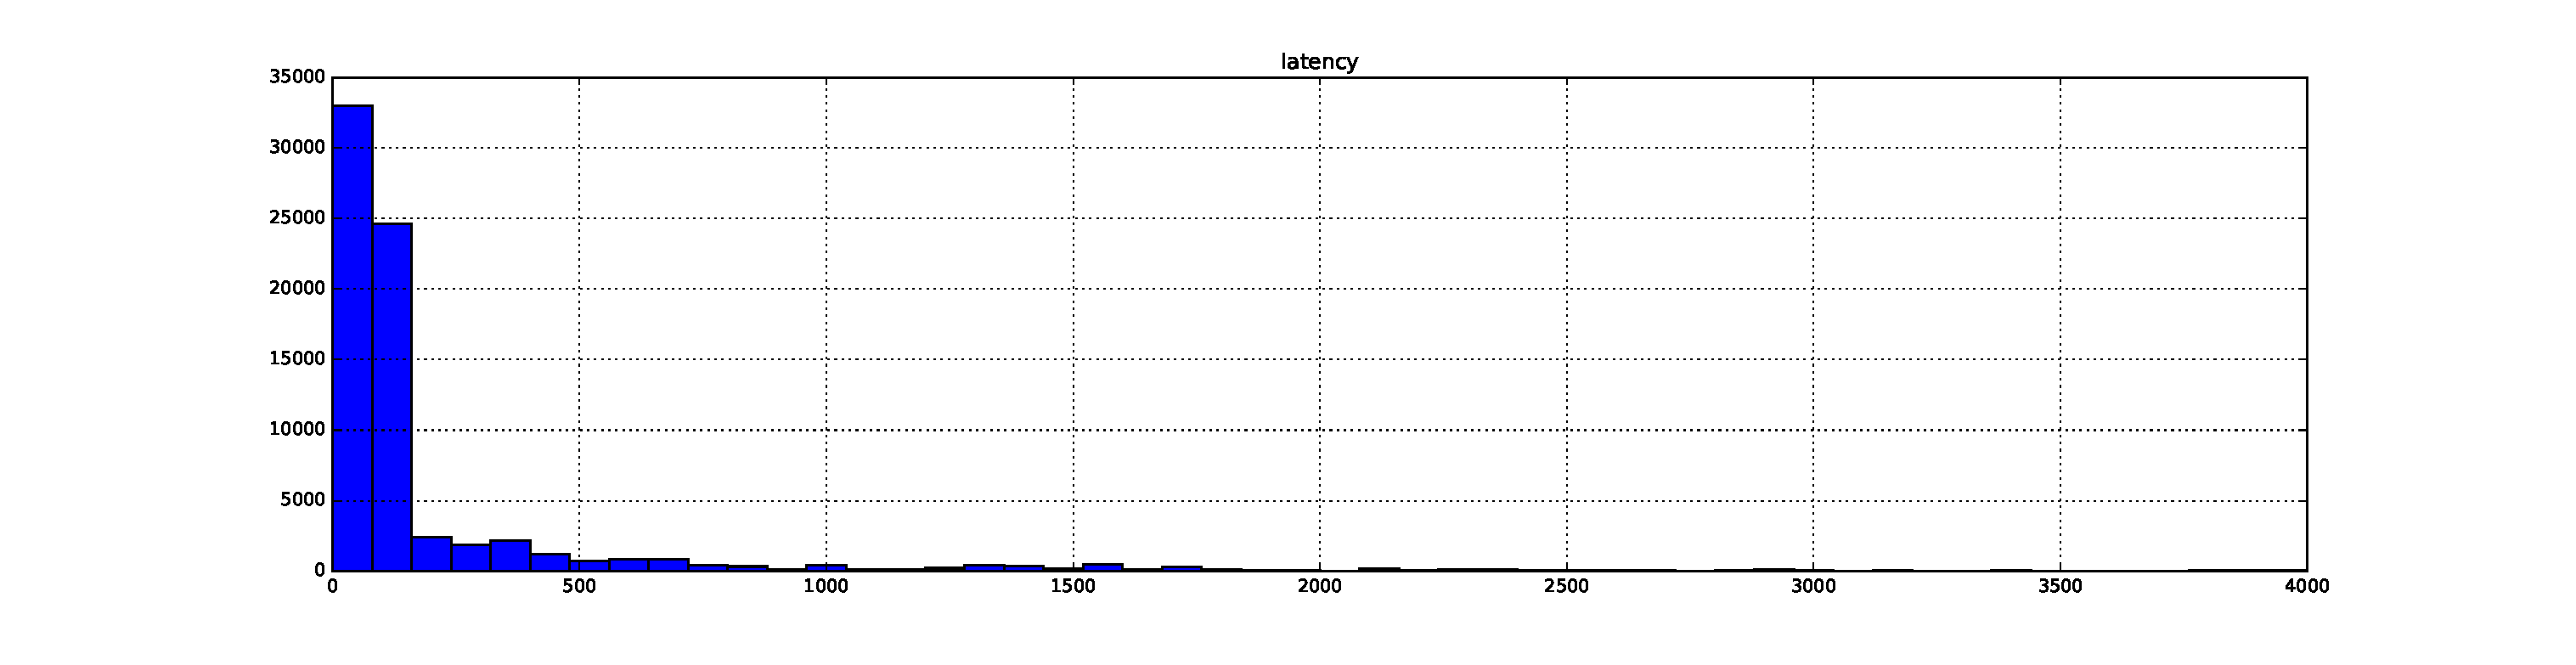
\includegraphics[width=\textwidth]{flink/8_1}
        \caption{8 Node latency histogram}
        \label{fig_partial_queue}
    \end{subfigure}


    \begin{subfigure}[b]{0.49\textwidth}
        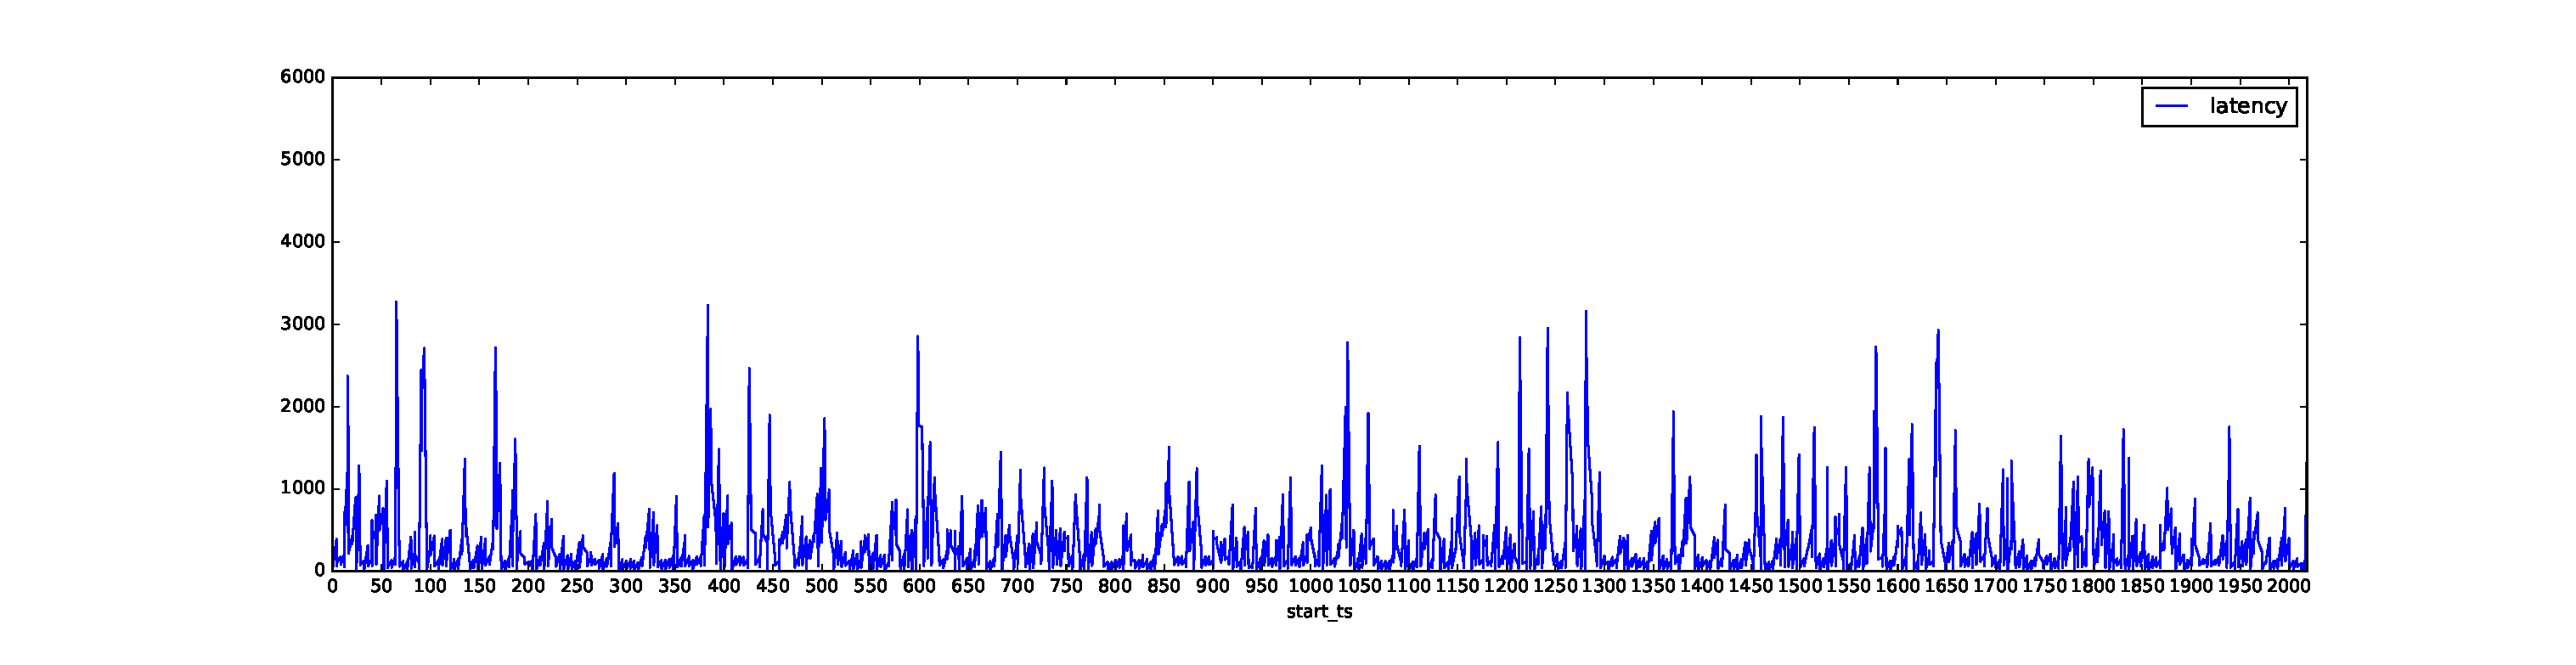
\includegraphics[width=\textwidth]{flink/2_2}
        \caption{2 Node latency time series}
        \label{fig_no_queue}
    \end{subfigure}
    ~ %add desired spacing between images, e. g. ~, \quad, \qquad, \hfill etc. 
      %(or a blank line to force the subfigure onto a new line)
    \begin{subfigure}[b]{0.49\textwidth}
        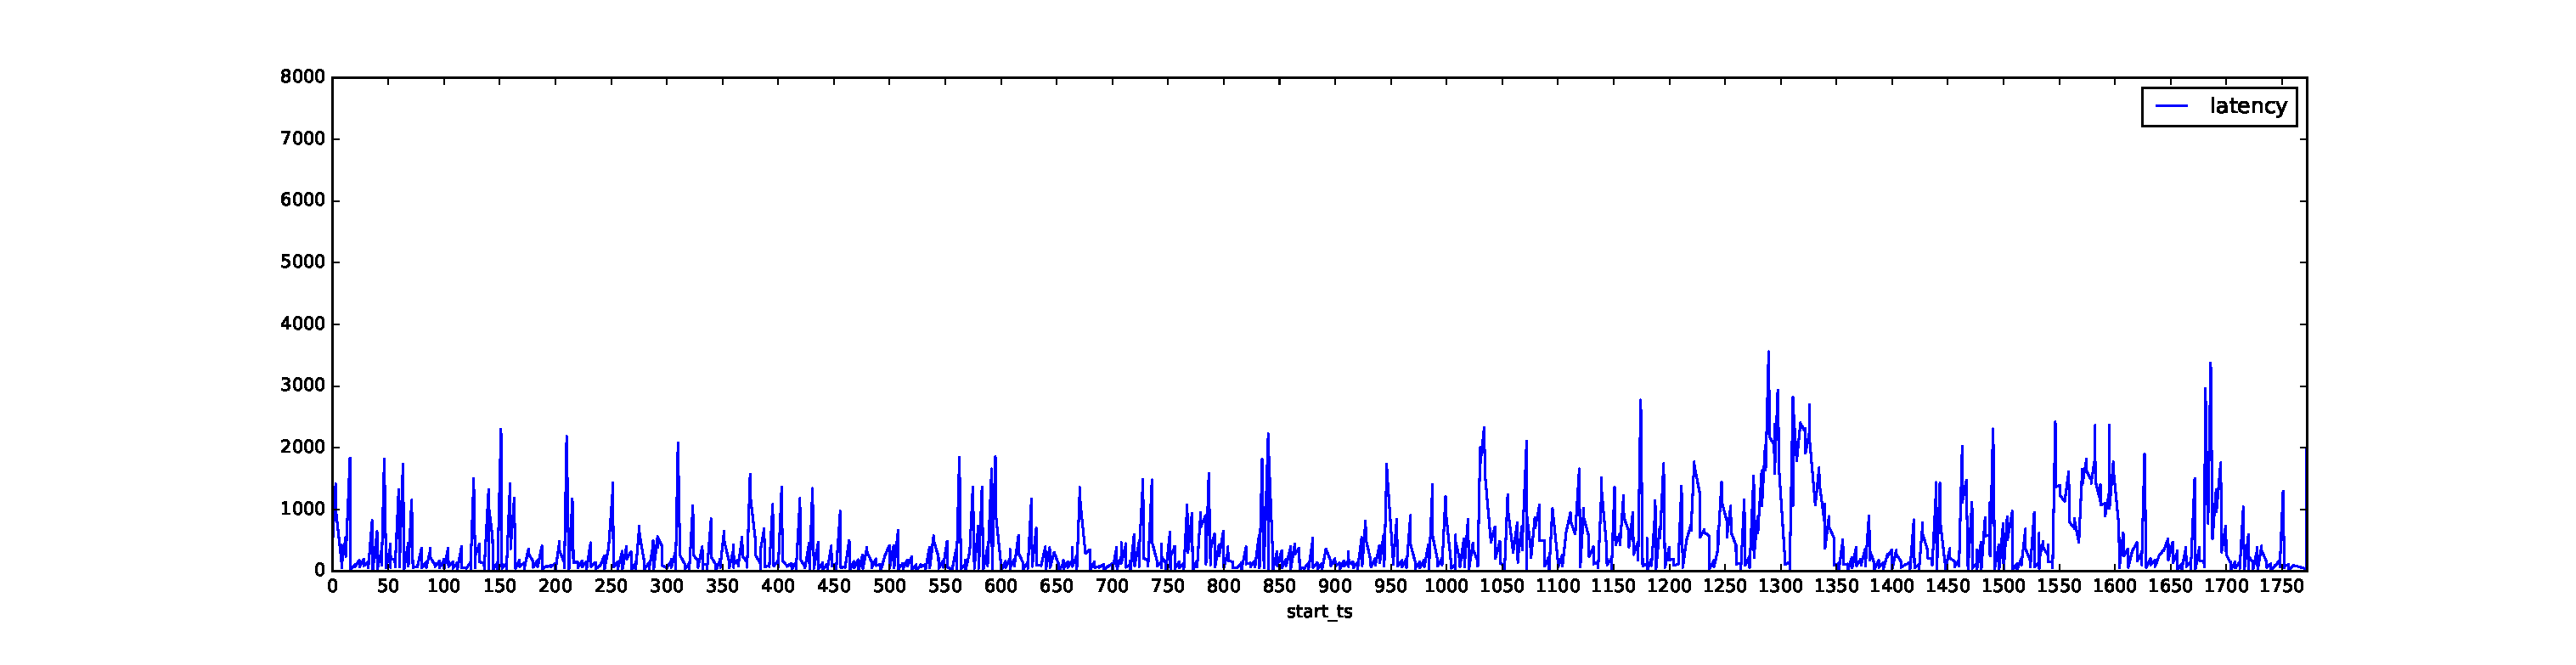
\includegraphics[width=\textwidth]{flink/3_2}
        \caption{3 Node latency time series}
        \label{fig_yes_queue}
    \end{subfigure}
    ~ %add desired spacing between images, e. g. ~, \quad, \qquad, \hfill etc. 
    %(or a blank line to force the subfigure onto a new line)
    \begin{subfigure}[b]{0.49\textwidth}
        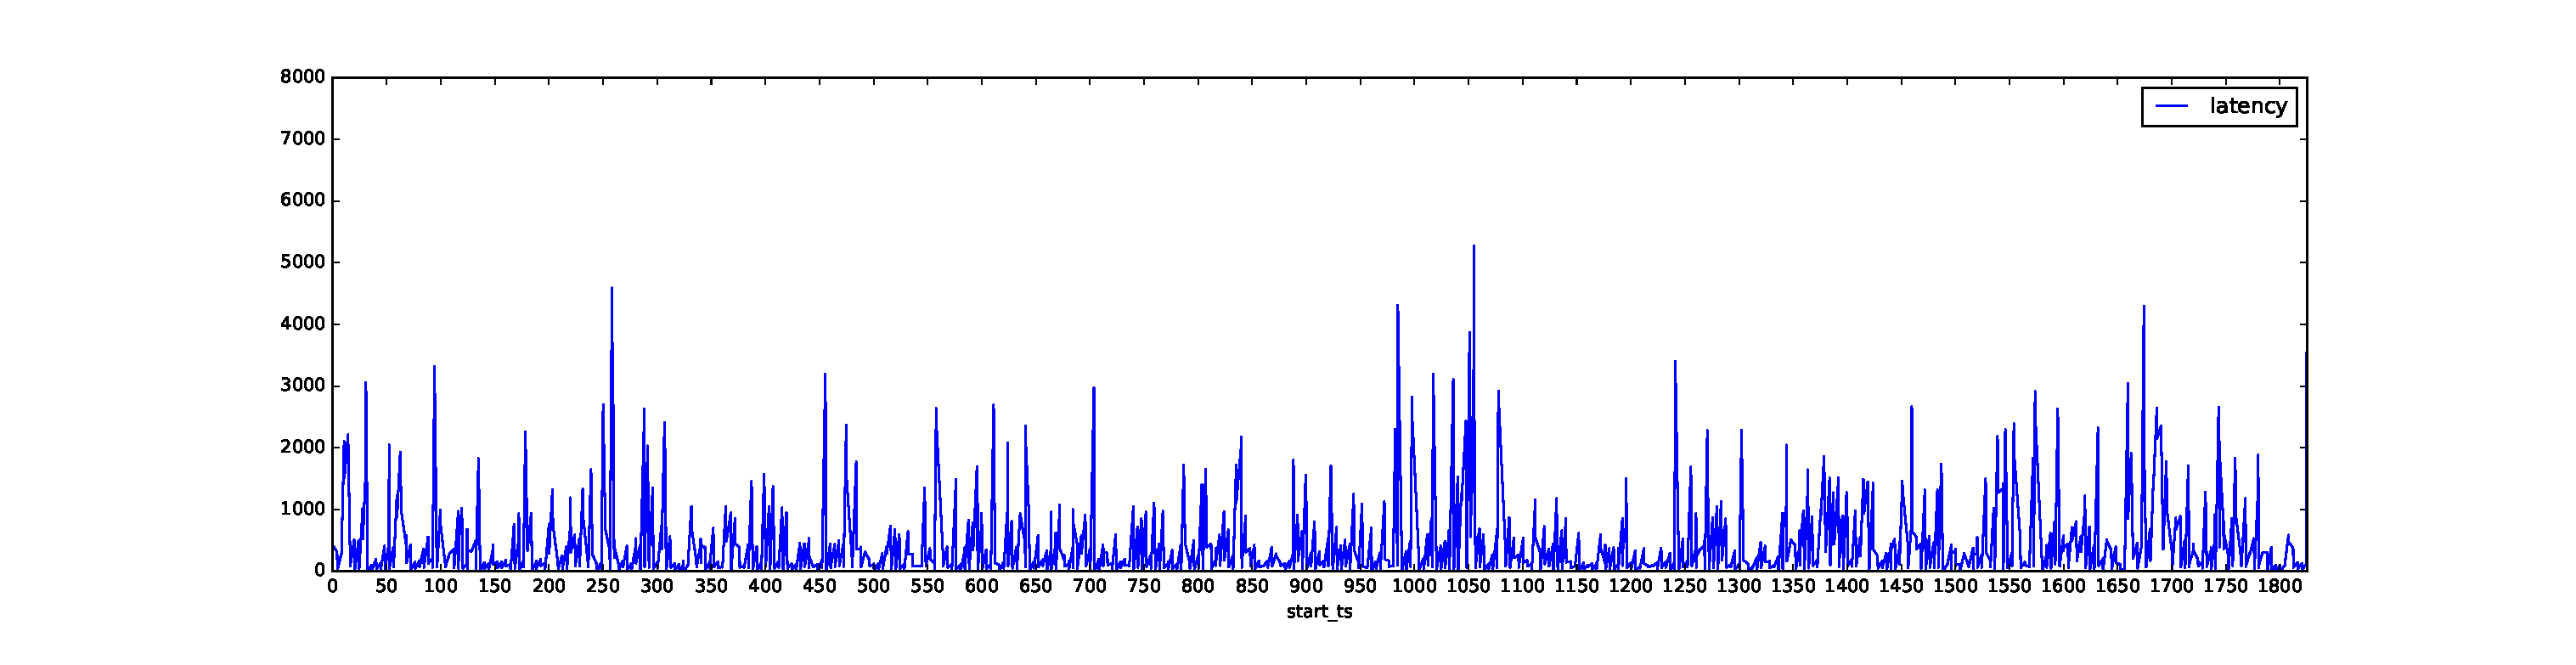
\includegraphics[width=\textwidth]{flink/4_2}
        \caption{4 Node latency time series}
        \label{fig_partial_queue}
    \end{subfigure}
        \begin{subfigure}[b]{0.49\textwidth}
        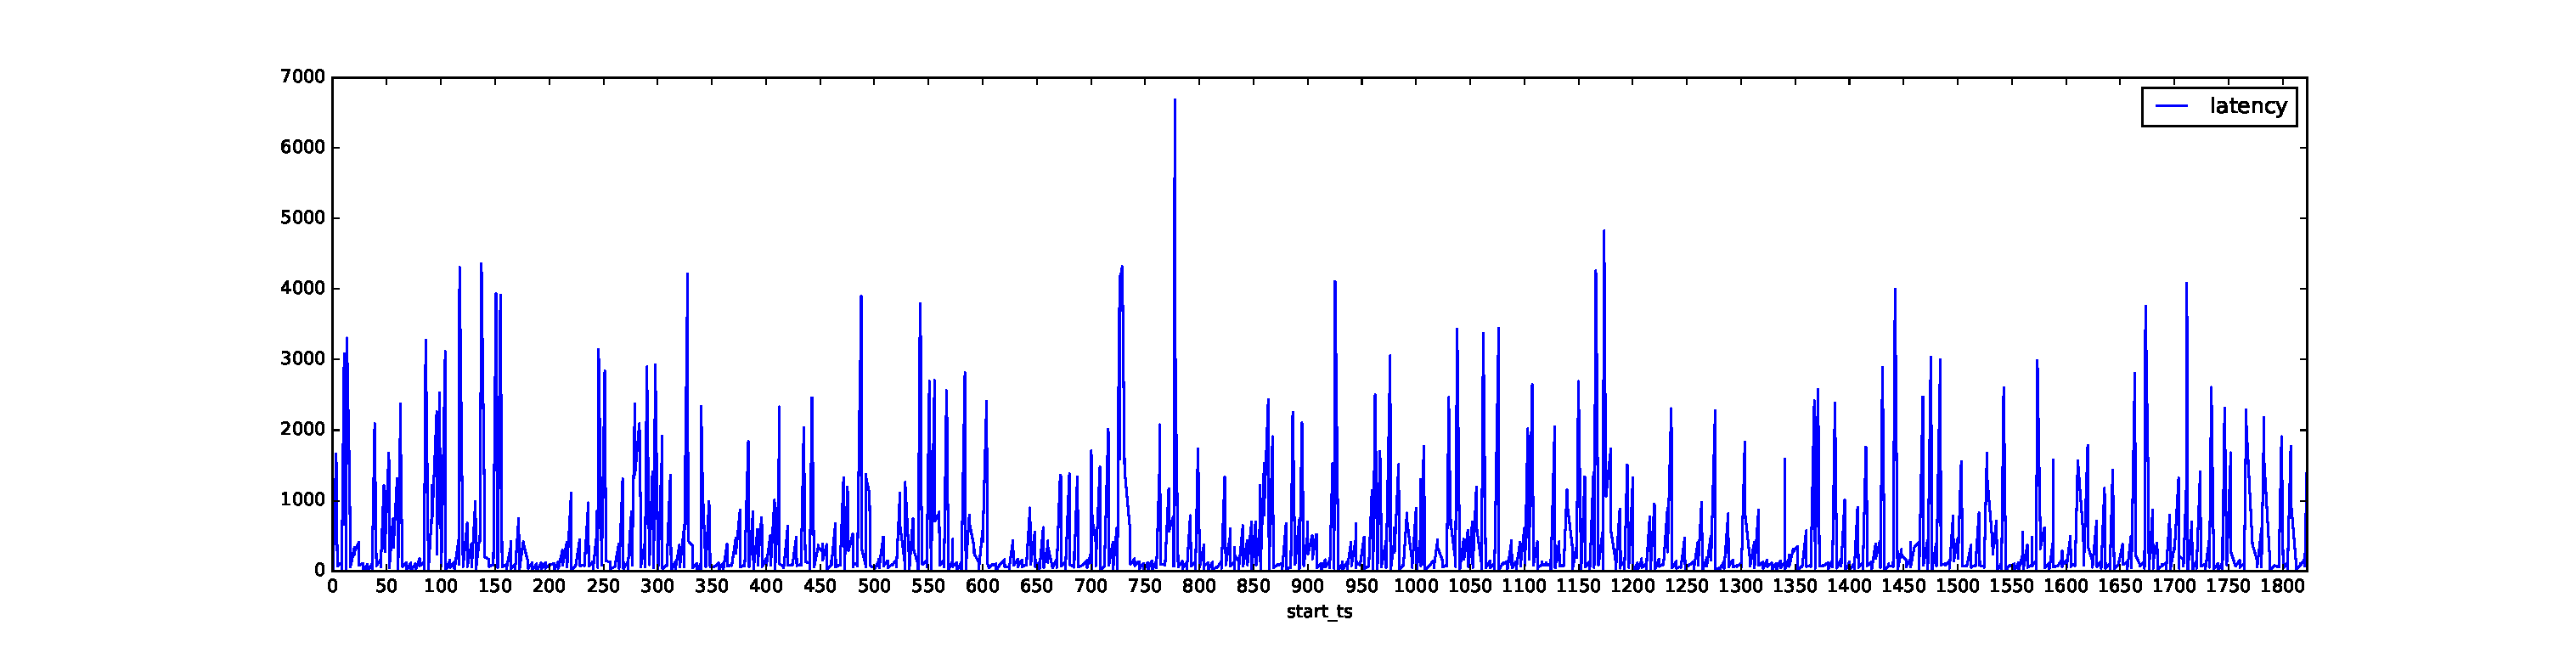
\includegraphics[width=\textwidth]{flink/8_2}
        \caption{8 Node latency time series}
        \label{fig_partial_queue}
    \end{subfigure}

    \label{fig_flink_agg_1}
        \caption{Latency of windowed aggregations for Flink.}
\end{figure*}


    \begin{table}
        \begin{tabular}{lllll}\toprule
            &\textbf{2 Node} & \textbf{3 Node} & \textbf{4 Node} & \textbf{8 Node}\\\midrule
            Storm & 345 & 235 & 345 & 345\\
            Spark(2sec) & 8K & 15K & 23K & 23K\\
            Spark(4sec) & 240K & 480K & 656K & 920K\\
            Flink & 1072K & 1232K & 1232K & 1232K\\
            \\\bottomrule
        \end{tabular}
        \caption{Sustainable throughput for windowed aggregations}\label{Tab1}
    \end{table} 

    \begin{table}
        \begin{tabular}{lllll}\toprule
            &\textbf{2 Node} & \textbf{3 Node} & \textbf{4 Node} & \textbf{8 Node}\\\midrule
            Storm & 345 & 235 & 345 & 345\\
            Spark(2sec) & 376 & 707 & 1.1K & 1.1K\\
            Spark(4sec) & 12K & 24K & 33K & 47K\\
            Flink & 53K & 58K & 58K & 58K\\
            \\\bottomrule
        \end{tabular}
        \caption{Average Window size for windowed aggregations}\label{Tab1}
    \end{table} 

    \begin{table}
        \begin{tabular}{lllll}\toprule
            &\textbf{2 Node} & \textbf{3 Node} & \textbf{4 Node} & \textbf{8 Node}\\\midrule
            Storm & 345 & 235 & 345 & 345\\
            Spark(2sec) & 1.6s & 1.7s & 1.7s & 1.6s\\
            Spark(4sec) & 6.9s & 3.6s & 4.4s & 3.9s\\
            Flink & 0.3s & 0.4s & 0.35s & 0.28s\\
            \\\bottomrule
        \end{tabular}
        \caption{Average Latency for windowed aggregations}\label{Tab1}
    \end{table} 


    \begin{table}
        \begin{tabular}{lllll}\toprule
            &\textbf{2 Node} & \textbf{3 Node} & \textbf{4 Node} & \textbf{8 Node}\\\midrule
            Storm & NULL & NULL & NULL & NULL\\
            Spark(2sec) & NULL & NULL & NULL & NULL\\
            Spark(4sec) & NULL & NULL & NULL & NULL\\
            Flink & 528K & 587K & 643K & 806K\\
            \\\bottomrule
        \end{tabular}
        \caption{Sustainable throughput for windowed joins}\label{Tab1}
    \end{table} 


    \begin{table}
        \begin{tabular}{lllll}\toprule
            &\textbf{2 Node} & \textbf{3 Node} & \textbf{4 Node} & \textbf{8 Node}\\\midrule
            Storm & NULL & NULL & NULL & NULL\\
            Spark(2sec) & NULL & NULL & NULL & NULL\\
            Spark(4sec) & NULL & NULL & NULL & NULL\\
            Flink & 3.6s & 4.7s & 4s & 3.4\\
            \\\bottomrule
        \end{tabular}
        \caption{Average Latency for windowed joins}\label{Tab1}
    \end{table} 


\subsection{Joins}





\begin{figure*}
    \centering
    \begin{subfigure}[b]{0.49\textwidth}
        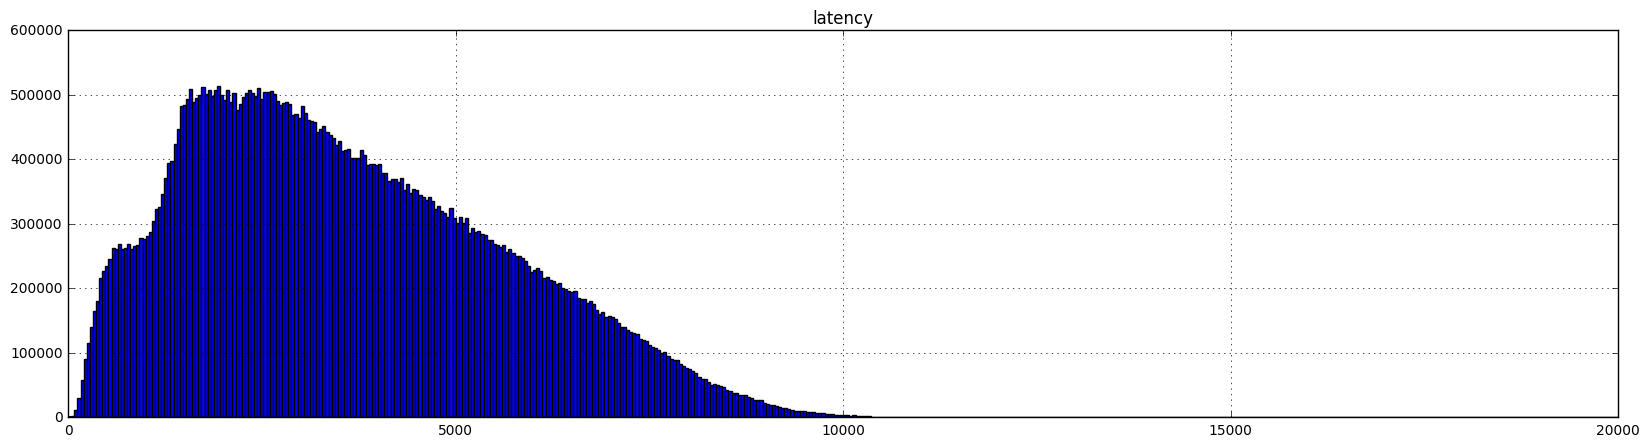
\includegraphics[width=\textwidth]{join/flink/2}
        \caption{2 Node latency histogram}
        \label{fig_no_queue}
    \end{subfigure}
    ~ %add desired spacing between images, e. g. ~, \quad, \qquad, \hfill etc. 
      %(or a blank line to force the subfigure onto a new line)
    \begin{subfigure}[b]{0.49\textwidth}
        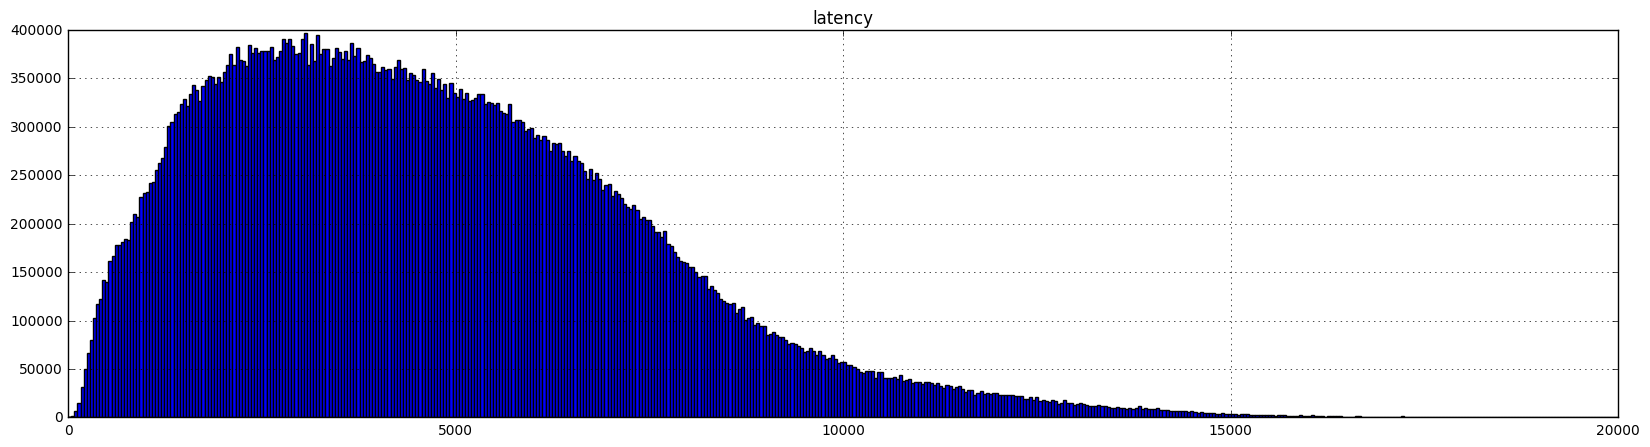
\includegraphics[width=\textwidth]{join/flink/3}
        \caption{3 Node latency histogram}
        \label{fig_yes_queue}
    \end{subfigure}
    ~ %add desired spacing between images, e. g. ~, \quad, \qquad, \hfill etc. 
    %(or a blank line to force the subfigure onto a new line)
    \begin{subfigure}[b]{0.49\textwidth}
        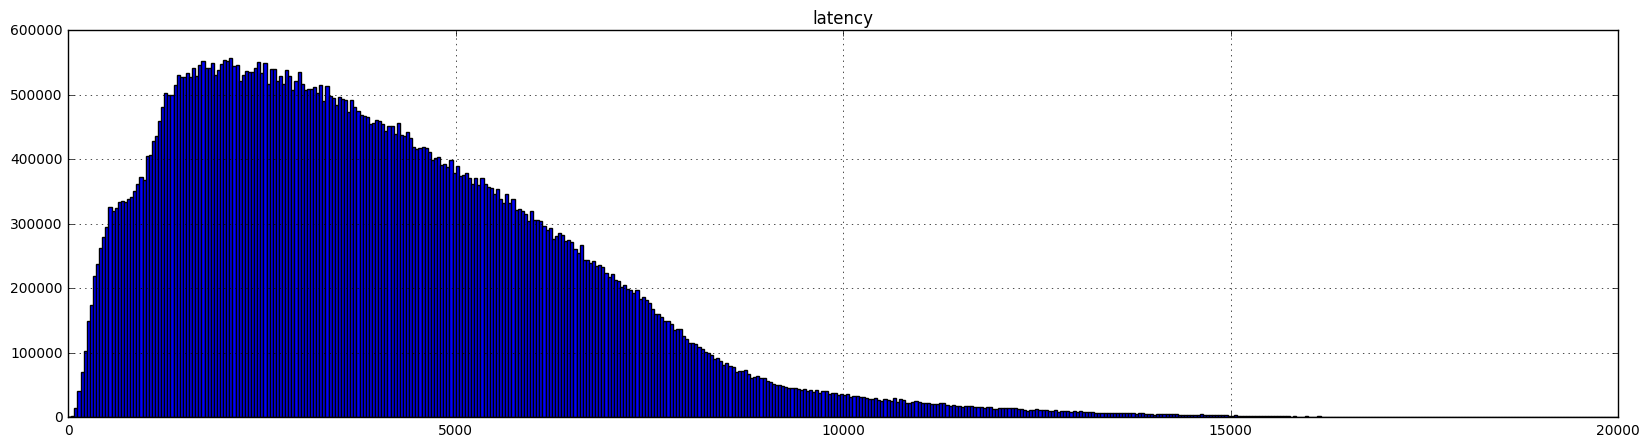
\includegraphics[width=\textwidth]{join/flink/4}
        \caption{4 Node latency histogram}
        \label{fig_partial_queue}
    \end{subfigure}
        \begin{subfigure}[b]{0.49\textwidth}
        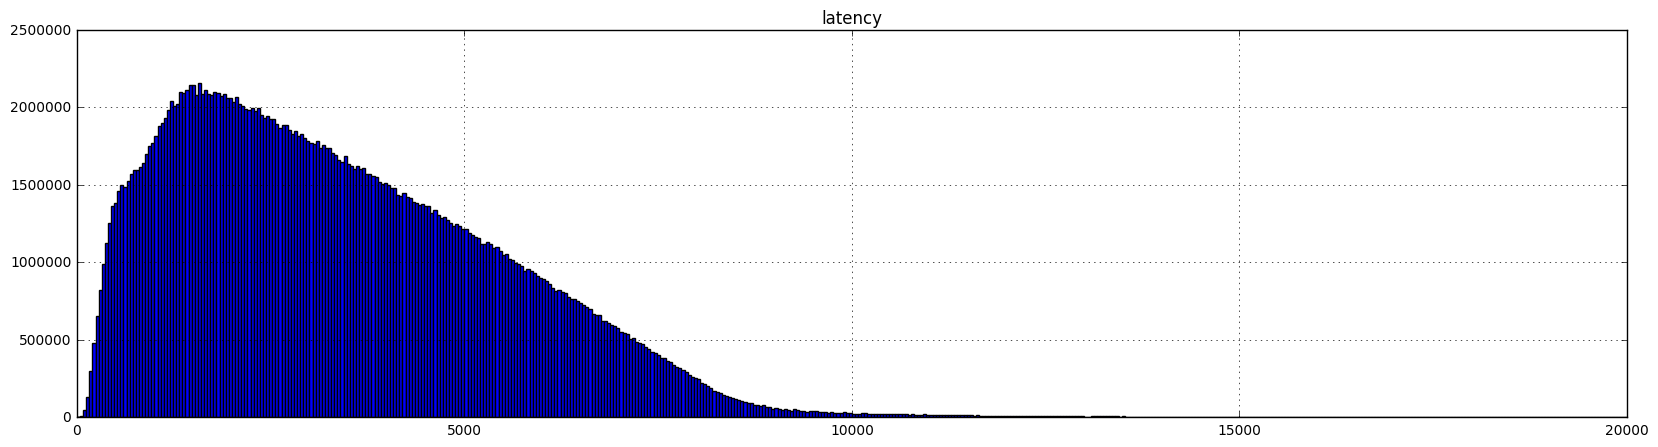
\includegraphics[width=\textwidth]{join/flink/8}
        \caption{8 Node latency histogram}
        \label{fig_partial_queue}
    \end{subfigure}



    \label{fig_flink_agg_1}
        \caption{Latency of windowed joins for Flink.}
\end{figure*}

\section{Conclusions}
\label{conc}

\section{Acknowledgments}

















% ensure same length columns on last page (might need two sub-sequent latex runs)
\balance

% The following two commands are all you need in the
% initial runs of your .tex file to
% produce the bibliography for the citations in your paper.
\bibliographystyle{abbrv}
\bibliography{vldb_sample}  % vldb_sample.bib is the name of the Bibliography in this case
% You must have a proper ".bib" file
%  and remember to run:
% latex bibtex latex latex
% to resolve all references


%APPENDIX is optional.
% ****************** APPENDIX **************************************
% Example of an appendix; typically would start on a new page
%pagebreak






\end{document}
